\documentclass[letterpaper, 10pt, conference]{ieeeconf}      % Use this line for a4
                                                          % paper

\IEEEoverridecommandlockouts                              % This command is only
                                                          % needed if you want to
                                                          % use the \thanks command
\overrideIEEEmargins
% See the \addtolength command later in the file to balance the column lengths
% on the last page of the document

%\setlength{\topmargin}{0.46in}


% The following packages can be found on http:\\www.ctan.org
\usepackage{graphics} % for pdf, bitmapped graphics files
\usepackage[dvips]{graphicx} % for eps
\usepackage{epsfig} % for postscript graphics files
%\usepackage{mathptmx} % assumes new font selection scheme installed
\usepackage{times} % assumes new font selection scheme installed
\usepackage{amsmath} % assumes amsmath package installed
%\usepackage{amssymb}  % assumes amsmath package installed
\usepackage{wasysym}
\usepackage{color}
\usepackage{algorithmic}
\usepackage{algorithm}
\usepackage{tensor}
\usepackage{leftidx}
\usepackage{subfigure}
\usepackage{supertabular}
%\renewcommand{\thesubfigure}{\thefigure.\arabic{subfigure}}
%\makeatletter
%\renewcommand{\p@subfigure}{}
%\renewcommand{\@thesubfigure}{\thesubfigure:\hskip\subfiglabelskip}
%\makeatother

%\usepackage[dvips, bookmarks=false, colorlinks=true, pdftitle={Hak-Humanoids2010}]{hyperref}
\newcommand{\mbf}[1]{{\mathbf{#1}}}
\newcommand{\dpartial}[2]{\frac{\partial{#1}}{\partial{#2}}}
\DeclareMathOperator*{\argmin}{arg\,min\,} 


\title{\LARGE \bf
Motion Analysis by Reverse Control for a Humanoid Robot
}

%\author{Sovannara Hak, Nicolas Mansard, Jean-Paul Laumond, Olivier Stasse% <-this % stops a space
  %\thanks{7 av col Roche, F-31077 Toulouse, France, Universit\'e de Toulouse; UPS, INSA, INP,
  %  ISAE: {\tt\small sovannara.hak@laas.fr, nicolas.mansard@laas.fr, jpl@laas.fr}. Olivier
  %  Stasse, CNRS-AIST, JRL (Joint Robotics Laboratory), UMI 3218/CRT,
  %  Intelligent Systems Research Institute AIST Central 2, Umezono 1-1-1
  %  Tsukuba, Ibaraki 305-8568 Japan: {\tt\small olivier.stasse@aist.go.jp}}
  %\thanks{This work was supported by a grant from the R-Blink Project, Contract
  %  ANR-08JCJC-0075-01.}  }


\begin{document}

\maketitle
\thispagestyle{empty}
\pagestyle{empty}


%%%%%%%%%%%%%%%%%%%%%%%%%%%%%%%%%%%%%%%%%%%%%%%%%%%%%%%%%%%%%%%%%%%%%%%%%%%%%%%%
\begin{abstract}
%Statistical approaches are widely used for motion recognition.
%However, those statistical methods need to be applied in a \emph{suitable} space.
Efficient methods to perform motion recognition have been developed
using statistical tools. Those methods rely on primitives learning
in a \emph{suitable space}, for example the latent space of the joint angle and/or the task space.
The learned primitives are sequential : a motion is segmented according to the time axis.
When working with a humanoid robot, a motion can be decomposed into
independent tasks for example in a waiter scenario,
the robot has to keep some plates horizontal with one of his arms, while placing a plate
on the table with his free hand.
In order to be able to recognize each combination of those kind of independent task,
the statistical approaches need to learn the primitives from the demonstrations of each
combinations of tasks.
%Being able to explain the motion makes sense when working with a humanoid robot for example,
%because the effectors of that kind of robot can be used to achieve various goal in
%a meaning point of view. The robot can move its hand, in order to grasp
%an object or to maintain balance.
The method presented here
takes advantage of the knowledge of what tasks the robot is able to do and how
the motion is generated from a known set of controllers to perform a reverse engineering of an
observed motion. This analysis is intended to recognize the simultaneous tasks that
have been used to generate a short motion. The method relies
on the task-function formalism and the projection operation into the null space of a task to decouple
the controllers.
The approach is successfully applied in simulation and on the real robot
to disambiguate motion in different scenarios where two motions look similar and have
different purposes.
\end{abstract}

\section{Introduction}
%\subsection{Motivation: what are you moving for?}

The current promising development of service robotics stimulates the
research in human-robot interaction. In that context, understanding
robot actions from observation is a challenge per se. While the
intentional action originates at a planning level, its realization takes
place in the real world via motions. How to recognize an action from
observed motions? Defining methods to automatically recognize the goal
pursued by a robot performing a given motion is a critical issue. If we
consider mobile manipulators (e.g., PR2 robots)
there is a clear separation between navigation functions and
manipulation functions. The question of action recognition may be rather
simple. Similarly humanoid robot can be divided in two distinctive parts,
legs and upper body, which corresponds to the navigation and manipulation
functions.

%\subsection{Problem statement: disambiguating motions in embodied actions.}
\begin{figure*}[t]
  \centering
  \makeatletter
  \renewcommand{\@thesubfigure}{Scenario \thesubfigure:\hskip\subfiglabelskip}
  \makeatother

  \subfigure[The global task \emph{Give me the ball} is decomposed into a
  sequence of sub-tasks \lbrack locate the ball\rbrack, \lbrack walk to the ball\rbrack, \lbrack grasp the
  ball\rbrack, \lbrack locate the operator\rbrack, \lbrack walk to the operator\rbrack, and \lbrack give the
  ball\rbrack. The motions \lbrack walk to\rbrack, \lbrack grasp\rbrack, \lbrack give\rbrack~appear as a sequence
  structuring the action.]{
  \makebox[\linewidth]{
  \begin{tabular}{c@{}c@{}c@{}c@{}c@{}}
    \includegraphics[height=2.4cm]{img/purpleBall1.ps}&
    \includegraphics[height=2.4cm]{img/purpleBall2.ps}&
    \includegraphics[height=2.4cm]{img/purpleBall3.ps}&
    \includegraphics[height=2.4cm]{img/purpleBall4.ps}&
    \includegraphics[height=2.4cm]{img/purpleBall5.ps}\\
  \end{tabular}
  \label{fig:introExample:purpleBall}
  }
  }
  \subfigure[To grasp the ball between its feet, the robot has to step
  away from the ball. In this experiment \emph{stepping away} is not a software
  module. It is an integral part of the embodied action \emph{grasping}]{
  \makebox[\linewidth]{
  \begin{tabular}{c@{}c@{}}
    \includegraphics[height=2cm]{img/graspFeet1.ps}&
    \includegraphics[height=2cm]{img/graspFeet2.ps}\\
  \end{tabular}
  \label{fig:introExample:graspFeet}
  }
  }
  \subfigure[To grasp the ball between in front of it (left), the robot
  reaches a posture where the left arm is used to maintain its balance. In
  the figure on the right, the robot performs two actions simultaneously:
  grasping a ball in front of it while grasping a ball behind (of course
  the ball behind has been intentionally placed at the end
  position of the left hand depicted on the left side). It
  is not possible to spot the difference between both postures. However,
  the question we address is: Is it possible to spot the difference
  between both \emph{motions}?]{
  \makebox[\linewidth]{
  \includegraphics[height=2.4cm]{img/spotDiff1H.ps}
  }
  \label{fig:introExample:spotDiff}
  }
  \caption{Introductory examples of embodied intelligence.}
  \label{fig:introExample}
\end{figure*}

For example, consider the \emph{Give me the purple ball} scenario~\cite{yoshida07}
performed by the humanoid robot HRP-2 at LAAS-CNRS (Fig.~\ref{fig:introExample}). To reach the assigned
objective, HRP-2 decomposes its task into elementary sub-tasks
(Fig.~\ref{fig:introExample:purpleBall}). A dedicated software module addresses each
sub-task. For instance,
to reach the ball, the robot has to walk to the ball. \emph{Walking} appears as an
elementary action that is a resource to solve the problem. It is processed by a
dedicated locomotion module. In the second scenario (Fig.~\ref{fig:introExample:graspFeet}),
HRP-2 has to grasp the ball that is located between its feet. To reach the
objective, the robot has to step away from the ball and then grasp it. In this
experiment~\cite{kanoun10} there is no dedicated module in charge of \emph{stepping}. \emph{Stepping} is
a direct consequence of \emph{grasping}. The grasping action is totally embedded in
the body, allowing the legs to naturally contribute to the action. Grasping
appears as an embodied action generating a complex motion. Finally Fig.~\ref{fig:introExample:spotDiff}
introduces the purpose of this paper. In the case on the left side, the robot
performs a single grasping task. In the case on the right side, the robot
performs two grasping tasks simultaneously. The ambiguity to distinguish both
cases comes from the role played by the left arm. In the first case, the left
arm contributes to the single grasping action by maintaining the balance of the
robot. In the second one, the left arm performs another grasping task. Both
motions are very similar. 

The works presented here tackles the problem of motion recognition and 
show that it is possible to disambiguate both cases by focusing
the analysis of the motion in the task spaces and on
the behaviors of the controllers of the robot.

In the following section, we review related works in task recognition applied
to humanoid robots. We then introduced in section~\ref{sec:sot} the basics of what the work presented here
relies on. The proposed algorithm to perform the motion analysis is presented in section~\ref{sec:detect}.
Finally, experimentations in simulation and on an HRP-2 robot that validate the method are presented in 
section~\ref{sec:simu} and section~\ref{sec:real}.

\section{Related work}
%In the quest of robot autonomy, research and development in Robotics is
%dominated by the stimulating competition between abstract symbol manipulation and physical signal
%processing, between discrete data structures and continuous variables.
%Indeed finding a proper way to relate the discrete space of symbols and the continuous space
%of controllers is a challenge.\\
%%%
Statistics have been successfully applied
to action recognition and motion analysis~\cite{schaal03}.
Statistical tools are used to create symbols, and by extension, detect those
symbols in a motion. For example, a method for behavior-based control 
is proposed in~\cite{drumwright03, drumwright04}. Behaviors are defined 
as a motion symbol (e.g. jab, hook, elbow, shield and uppercut). 
The behaviors are modeled by learning from series of examples.
A dimensional reduction is then applied to have a significant
clusterization.  The recognition part is handled by a Bayesian classifier which
recognize a trajectory in joint or Cartesian space. The extension to the recognition
is to perform an imitation. This is performed by interpolating known examples to obtain
feasible trajectories. The introduction of Partially
Observable Markov Decision Process or Bayesian inference~\cite{pearl88} has
renewed the topic of action modeling~\cite{kaelbling98} in the last decade. Such
techniques and related ones are now applied to motor skill learning~\cite{peters08} in
general, and to motion segmentation~\cite{calinon10, inamura04} in particular. 
Generally speaking, the efficiency of statistics based recognition is ruled by the quality of the dataset built
in the learning phase.
Several demonstrations for each particular cases is needed to be able to extract
the invariants that will discriminate the tasks. The sparsity of the demonstrations
can also limits the efficiency of the recognition. Finally, the sets of demonstrations
have to be associated with the correct symbols, which is generally given to the learning algorithm.

Alternatively, recognition can be based on specific criteria that are given as 
a priori to the system. In~\cite{nakaoka07}, only the robot trajectories
are used to distiguish between various phases of motion. A task is
a complete motion within a temporal segment. The global motion
is a sequence of tasks. Each task has its own
parameters called \emph{skills parameters}. The task recognition method is decomposed in two steps: 
first, for each tasks, find all the temporal segments in the observed motion
corresponding to that task.
The second step is the estimation of the skill parameters for each segment.
Each task are detected by the analysis of a trajectory projected in a specific space.
For example, the stepping task is detected by analyzing the trajectory 
of a foot; a squatting task is detected by analyzing the vertical trajectory of the waist.
However, the criteria used for detection and the associated dedicated projection spaces
are ad-hoc, built manually for a particular motion that has to be imitated by the robot.

Similarly,~\cite{muhlig09} uses a set of specific spaces
in which the observed motion is projected and where ad-hoc criteria
%Observations of a movement from sensors (camera, or motion capture system)
are computed to map to the union of task spaces that will best represent and generalize the movement in order to focus
a learning technique into that new space. The task space selection is
done by computing score functions inspired by neuroscience: the proposed criteria are
the saliency of the object that is manipulated, a variance of the dimension
of a space during several demonstrations, and some heuristics that express that
uncomfortable or exhausting motions are more relevant to a task. Those heuristics
address the problem of how to spot tasks that involve no motion. The method
presented add some higher level information to a purely statistical analysis. However
the efficiency of the task space selection depends on the strength
of the heuristics.

The common approach of these last works are to project the observed motion in some specific reduced spaces,
where the recognition is easier. These spaces can be chosen arbitrary~\cite{nakaoka07}, 
automatically selected~\cite{muhlig09} or learned~\cite{peters08}. Similarly, in control,
smaller-size spaces are used to define the control objectives and modulate the robot behavior.
A task function~\cite{samson91} expresses a control objective in a $n-\text{dimensional}$ task space.
The approach has been extended to handle a hierarchical set of tasks~\cite{siciliano91, nakamura87},
and to the operational space control~\cite{khatib87} using the redundancy of a system.

%In this work the control law is obtained by a \emph{stack of tasks}
%(SoT)~\cite{mansard07} ie hierarchical inverse kinematics
%\cite{siciliano91}.\\                                       

%In this paper another point of view is taken: the control theory based
%one. Control theory constitutes the second corpus that accompanies
%robotics development. Originating from mechanics and applied
%mathematics, it focuses on robot motion control~\cite{murray94,
%siciliano10}. Among all the
%contributions on linear and non-linear systems, robot control theory has
%provided efficient concepts for motion generation. The research
%initiated by A. Li\'egeois~\cite{liegeois77} on redundant robots (i.e. robots that have
%more degrees of freedom than necessary to perform a given task), and
%then developed by Y. Nakamura~\cite{nakamura91}, B. Siciliano, J.J. Slotine~\cite{siciliano91} and O.
%Khatib~\cite{khatib87} introduce mathematical machinery based on linear algebra and
%numerical optimization that allows for clever ways to model the symbolic
%notion of \emph{task}~\cite{samson91}.\\

%Those \emph{tasks} are defined by their tasks spaces (eg. position of the hand
%in an arbitrary frame\cite{nakamura86a,khatib87}, or position of a visual feature in the image
%plane \cite{espiau92,hutchinson96a}), a reference behavior in those tasks spaces
%(eg. exponential decrease to zero) and by the differential link between
%the task space and the actuator space, typically the task Jacobian.
%Given a set of active task, the corresponding control law can be
%obtained by inverting the equation of motion of the robot. 

%In this work, the analyzed motion is not seen as a sequence of motion primitives but as a
%superimposition of controllers. The recognition of sequences
%is out of the scope of the paper.
%The task-function is generally used to generate a motion\cite{siciliano91, mansard07}, and
The originality of the method presented in this paper is to use the properties of the
task-function to perform a recognition. The main idea is
to perform a reverse engineering of an observed motion knowing the set of all possible tasks that can appear 
in a motion using their reference behaviors as characteristic trajectories. 
The motion that is supposed to be generated by stacking the objectives controls is processed in order to
seek the known behaviors. The analysis is performed in each task spaces. 
Moreover, while all the approaches presented above can only deal with non-simultaneous task to recognize,
we can rely on the redundancy-control principles to recognize sets of simultaneous tasks.
Projections of the motion in orthogonal spaces of already detected tasks
ensure an efficient decoupling of the tasks performed
by the robot.
%The control law associated to the task function approach can be decomposed in two components:
%a main command and a secondary command.
%The secondary command is computed so as to not interfere with the main command. This is classically achieved by
%projecting secondary commands into the nullspace of the main command. All degrees of freedom
%that are not used by the main command will be used to achieve other commands.
%In this work, instead of using the projector onto the nullspace of a task to generate a new control law that takes into
%%account some lower priorities commands, the projector is used on a joint angle trajectory
%to remove the part of the motion that corresponds to a detected task, removing
%ambiguity produced by combination of tasks. Furthermore, the recognition method is
%performed in each known task spaces in order to analyze trajectories in appropriate spaces.\\
%
%The next section sum up the basics notions related to the task-function
%formalism used throughout this paper. The proposed algorithm for the task recognition
%is detailed in section~\ref{section:algorithm}. Section~\ref{sec:simu} and~\ref{section:real}
%illustrates the method respectively in simulation and on the real robot followed
%by concluding remarks.

\section{Tasks and stack of tasks}
\label{sec:sot}
A task function~\cite{samson91} is an elegant approach to describe intuitively
sensor-based control objectives. Based on the redundancy of the system, the
approach can be extended to consider a hierarchical set of
tasks~\cite{siciliano91}.  Defining the motion of the robot in terms of tasks
consists in choosing several control laws to be applied each on a different
subspace of the robot degrees of freedom. 

A task is defined by a vector space 
$\mbf{e}$ and by the reference behavior $\mbf{\dot{e}}$ to be
executed in the task space. The Jacobian of the task is noted
$\mbf{J}=\dpartial{\mbf{e}}{\mbf{q}}$ where $\mbf{q}$ is the robot
configuration vector. 
For a reaching task in three dimensions, $\mbf{e}$ is the error 
between a signal $\mbf{s}$ and its desired value
\begin{eqnarray*}
  \mbf{e} & = & \mbf{s}^* - \mbf{s} = \mbf{p}_3^* - \mbf{p}_3\\
  \mbf{J} & = & \dpartial{\mbf{p}}{\mbf{q}}\\
  \mbf{\dot{e}}^* & = & -\lambda \mbf{e}, \text{with } \lambda>0
\end{eqnarray*}
When the input control is the velocity
$\mbf{\dot{q}}$, the control law is given by the least-square solution:
\begin{equation}
\dot{\mbf{q}} = \mbf{J}^+ \mbf{\dot{e}}^* + \mbf{P}\mbf{z}
\end{equation}

\noindent where $\mbf{J}^+$ is the least-square inverse of $\mbf{J}$,
$\mbf{P} = \mbf{I} - \mbf{J}^+ \mbf{J}$ is the projection operator onto the null space
of $\mbf{J}$ and $\mbf{z}$ is any secondary criterion. $\mbf{P}$ ensures
a decoupling of the task with respect to $\mbf{z}$. 
using $\mbf{z}$ as a secondary input, the control can be extended
recursively to a set of \emph{n} tasks. Those \emph{n} tasks
are ordered by priority : task number 1 being the highest priority task,
and task number \emph{n}, the lowest priority.
In other word, $task_i$ should not disturb $task_j$ if $i>j$.
The recursive formulation of the control law is proposed by~\cite{siciliano91} :
\begin{equation}
\dot{\mbf{q}}_i = \dot{\mbf{q}}_{i-1} + (\mbf{J}_i \mbf{P}_{i-1}^{A})^+
(\dot{\mbf{e}}^*_i - \mbf{J}_i \dot{\mbf{q}}_{i-1}) , \ \ i = 1 \ldots n
\end{equation}
\noindent with $\dot{\mbf{q}}_0 = 0$ and $\mbf{P}_{i-1}^{A}$ is
the projector onto the null space of the augmented Jacobian
$\mbf{J}_i^A = (\mbf{J}_1, \ldots \mbf{J}_i)$. The robot
joint velocity realizing all the tasks is $\dot{\mbf{q}}^* = \dot{\mbf{q}}_n$.
A complete implementation of this approach is proposed in~\cite{mansard07} under the
name \emph{Stack of Tasks} (SoT). 

\section{Motion analysis for task recognition} 
\label{sec:detect}
\label{section:algorithm}
The algorithm proposed in this section
is used to perform task recognition for a humanoid robot by
identifying the set of tasks that have been used to
generate the observed motion.

\subsection{Hypothesis}
It is assumed that the model behavior of a task is known, so the distance between
the theoretical and the actual trajectory measure how close an actual trajectory is
to a trajectory generated by a controllers.
The model of the robot and all tasks that may appear in a motion (the tasks pool) are known.
The observed motion is generated using a sub-set of those tasks.  
It is also assumed that all the tasks involved in a motion are compatible:
each tasks are completely fulfilled. 

\subsection{Overview}
\label{sec:alg1:selec}
The input of the algorithm is a joint angle trajectories, and a set of candidate
tasks. The algorithm is iterative: at each iteration, the task that seems the
most relevant is selected. The selection of a task relies
on a curve fitting score : a projected trajectories is 
compared to a theoretical trajectory which represents a characteristic
trajectory of the execution of a task.
The projectors decouple their associated tasks in the motion.
As a consequence, they can be used to iteratively recognize
simultaneous tasks. The observed motion is projected
onto the null-space of the selected task, cancelling it in the motion,
and the other tasks can iteratively be recognized using the same mechanism in the projected motion.
The algorithm stops when the original
motion is totally canceled by the successive task cancellation.

The algorithm is showed in Alg.~\ref{alg:taskSelection}.
The joint angles velocities trajectory
of the motion to analyze is denoted $\mathbf{\dot{q}}^{*}(t)$,
$\mathbf{P}$ denotes a projector, $\mathbf{\dot{q}}(t)$ the angle velocity trajectory
of the reference motion, $r_i$ the score of the cost function of the optimization, $activePool$
the set of tasks selected during the algorithm and $\epsilon$ the threshold
of the motion norm below which the algorithm stops. The task fitting is described
in the following section. The procedure $\mathrm{projection}(i, \mathbf{\dot{q}}(t))$ compute the projector onto
the null space of the task $i$ and apply the projection to the motion.

\newcommand{\shOUTPUT}{\textbf{Output: }}
\newcommand{\shINPUT}{\textbf{Input: }}

\begin{algorithm}
  \caption{Task selection algorithm}
  \label{alg:taskSelection}
\begin{algorithmic}[1]
  \STATE \shINPUT $\mathbf{\dot{q}}^{*}(t)$
\STATE \shOUTPUT $activePool$
\STATE $\mathbf{P}\mathbf{\dot{q}}(t)\gets \mathbf{\dot{q}}^{*}(t)$
\WHILE{$\int \Vert \mathbf{P}\mathbf{\dot{q}}(t) \Vert ^2 dt > \epsilon$ }
  \FOR{task $i = 1..n$}
    \STATE $r_i \gets \mathrm{taskFitting}(i)$
  \ENDFOR
  \STATE $i_{select} \gets \mathrm{argmin}(r_i)$
  \STATE $activePool.\mathrm{push}(i_{select})$
  \STATE $\mathbf{P}\mathbf{\dot{q}}(t) \gets \mathrm{projection}(i_{select}, \mathbf{P}\mathbf{\dot{q}}(t))$
\ENDWHILE
\end{algorithmic}
\end{algorithm}

\subsection{Task fitting by optimization} \label{sec:alg2:proj}
The quantification of the relevance of a given task, with respect to
the execution of a motion, is achieved by applying a least-square optimization
between the actual motion and the reference behavior of a task over the parameters
of the reference behavior :
\begin{equation}
	\mbf{x}^* = \underset{\mbf{x}}\argmin \frac{\Vert \mbf{p}^*(t) - \mbf{p}_\mbf{x}(t) \Vert^2}{\Vert \mbf{p}^*(t) \Vert^2}
\label{optimProblem}
\end{equation}

\noindent where $\mbf{p}^*(t)$ is the reference trajectory, $\mbf{p}_\mbf{x}(t)$ is the trajectory
generated by the model using the parameters $\mbf{x}$. The CFSQP solver has been used in this work~\cite{lawrence97}.
It has to be noted that all trajectories lie in the relevant task space.

The task reference behavior $\mbf{\dot{e}}$ can, for example, be defined by an exponential regulation.
For the humanoid robot, the characteristic trajectory in the task
space is modeled by an
exponential decrease with 3 input parameters :

\begin{equation}
p_{\mbf x}(t) = x_1 \mathrm{e}^{(-x_2 t)} + x_3
\label{eqTask}
\end{equation}

This is motivated by the nature of the control of the
robot.\\

\subsection{Projection of the motion}
In this section, we demonstrate that the order of projections
has no influence as long as the tasks are the tasks involved
are completely fulfilled.

\section{Results in simulation}
\label{sec:simu}
This section details a series of experimentation in simulation related to this work.
The first experiment validates the projection of the motion.
The second compiles a set of experiments that validate the task recognition algorithm. For each
experiment of that set, the task recognition algorithm proposed in this paper
is applied to two similar motions.
The two motions have been artificially built to be ambiguous when 
they are compared to each other, in order to illustrate the 
efficiency of the algorithm regarding the precision of the recognition.
All motions involved in the experiments are summed up in table~\ref{tab:motion}.
They are generated by using the model of the humanoid robot HRP-2 
having 30 actuated degrees of freedom (plus 6 degrees of freedom on the
freeflyer). All motions start from the half-sitting pose showed in Fig.~\ref{fig:halfSit}.
As classically done in inverse kinematics, the under-actuation of the freeflyer is resolved by constraining
the left foot to be on the ground. The description of the tasks are detailed in the following.

\subsection{Notations}
The set of tasks considered in those experiments are :

\begin{itemize}
  \item \emph{Com} : the center of mass of the robot is constraint to maintain the static balance
  \item \emph{Gaze} : the robot looks at one point in the Cartesian space
  \item \emph{Twofeet}: constraint the both feet to stay flat on the ground
  \item \emph{Left/right grab} : is a reaching task, either the left or right hand
of the robot reaches a point defined in the Cartesian space
  \item \emph{Screw} : is similar to the \emph{grab} task, but the desired position
has to be reached with a defined orientation.
  \item \emph{Head} : is reaching task constrained in position and orientation with the head of the
    robot.
  \item \emph{Chest} : the chest of the robot is constrained in orientation.  
\end{itemize}
\begin{figure}[t]
\begin{center}
\includegraphics[width=0.3\linewidth]{img/halfSit.ps}
\end{center}
\caption{All reference motions start from a half-sitting pose.}
\label{fig:halfSit}
\end{figure}

The motion generated for the experiments are summed up in Table~\ref{tab:motion}.
Each experimentation will involve two motions (\emph{motion a} and \emph{motion b}) 
that have a small difference in the
stack of tasks used to generate the motion in order to illustrate
the efficiency of the disambiguation.

\begin{table}
  \centering
    \begin{tabular}{|c|c|c|}
      \hline
      & (a) & (b) \\
      \hline
      & &
      \\
      Motion 1 & 
	\begin{tabular}{|c|}
          \hline
          \emph{Right grab}\\
          \hline
          \emph{Left grab}\\
          \hline
          \emph{Gaze}\\
	  \hline
	  \emph{Com}\\
	  \hline
	  \emph{Twofeet}\\
	  \hline
	\end{tabular} & \\
      & &
      \\
      \hline
      & &
      \\
      Motion 2 & 
        \begin{tabular}{|c|}
          \hline
          \emph{Right grab}\\
	  \hline
	  \emph{Com}\\
	  \hline
	  \emph{Twofeet}\\
	  \hline
	\end{tabular}  
    &
	\begin{tabular}{|c|}
	  \hline
	  \emph{Left grab}\\
	  \hline
	  \emph{Right grab}\\
	  \hline
	  \emph{Com}\\
	  \hline
	  \emph{Twofeet}\\
	  \hline
	\end{tabular}  
    \\
    & &
    \\
    \hline
    & &
    \\
    Motion 3 & 
        \begin{tabular}{|c|}
	  \hline
	  \emph{Gaze}\\
	  \hline
	  \emph{Right grab}\\
	  \hline
	  \emph{Com}\\
	  \hline
	  \emph{Twofeet}\\
          \hline
        \end{tabular}  
    &
	\begin{tabular}{|c|}
	  \hline
	  \emph{Gaze}\\
	  \hline
	  \emph{Right screw}\\
	  \hline
	  \emph{Com}\\
	  \hline
	  \emph{Twofeet}\\
	  \hline
	\end{tabular}  
    \\
    & &
    \\
    \hline
    & &
    \\
    Motion 4 & 
	\begin{tabular}{|c|}
	  \hline
	  \emph{Left screw}\\
	  \hline
	  \emph{Com}\\
	  \hline
	  \emph{Twofeet}\\
	  \hline
	\end{tabular}  
    &
	\begin{tabular}{|c|}
	  \hline
	  \emph{Gaze}\\
	  \hline
	  \emph{Com}\\
	  \hline
	  \emph{Twofeet}\\
	  \hline
	\end{tabular} 
      \\
    & &
    \\
    \hline
    & &
    \\
    Motion 5 &
    \begin{tabular}{|c|}
      \hline
      \emph{Right grab}\\
      \hline
      \emph{Gaze}\\
      \hline
      \emph{Com}\\
      \hline
      \emph{Twofeet}\\
      \hline
    \end{tabular}
    &
    \begin{tabular}{|c|}
      \hline
      \emph{Right grab}\\
      \hline
      \emph{Chest}\\
      \hline
      \emph{Com}\\
      \hline
      \emph{Twofeet}\\
      \hline
    \end{tabular}
    \\
    & &
    \\
    \hline
  \end{tabular}
  \caption{Table of motions generated by their associated stack of tasks.}
  \label{tab:motion}
\end{table}

\subsection{Experiment 1 : Preliminary validation}
In this experiment, a basic composed motion is generated. Then the recognition by fitting
and the termination condition of the algorithm are validated.
The reference motion is the \emph{motion 1.a} (see~\ref{tab:motion}).

The motion is given to the detection program
which select the tasks that are fitted the best by the optimization.

Fig.~\ref{fig:snapshotXpqdot} shows snapshots during the original motion,
and the motions after successive projections
in the null spaces of the detected
tasks : \emph{right grab}, \emph{Com}, \emph{gaze}, \emph{Twofeet} and \emph{left grab}.
\begin{figure*}[t]
\centering
\begin{tabular}{c@{}c@{}c@{}c@{}c@{}c@{}c}
(a)&
\parbox[c]{2.4cm}{\includegraphics[width=\linewidth]{img/Pqdot0_0.png.ps}} &
\parbox[c]{2.4cm}{\includegraphics[width=\linewidth]{img/Pqdot0_99.png.ps}} &
\parbox[c]{2.4cm}{\includegraphics[width=\linewidth]{img/Pqdot0_199.png.ps}} &
\parbox[c]{2.4cm}{\includegraphics[width=\linewidth]{img/Pqdot0_299.png.ps}} &
\parbox[c]{2.4cm}{\includegraphics[width=\linewidth]{img/Pqdot0_399.png.ps}} &
\parbox[c]{2.4cm}{\includegraphics[width=\linewidth]{img/Pqdot0_499.png.ps}}\\

(b)&
\parbox[c]{2.4cm}{\includegraphics[width=\linewidth]{img/Pqdot1_0.png.ps}} &
\parbox[c]{2.4cm}{\includegraphics[width=\linewidth]{img/Pqdot1_99.png.ps}} &
\parbox[c]{2.4cm}{\includegraphics[width=\linewidth]{img/Pqdot1_199.png.ps}} &
\parbox[c]{2.4cm}{\includegraphics[width=\linewidth]{img/Pqdot1_299.png.ps}} &
\parbox[c]{2.4cm}{\includegraphics[width=\linewidth]{img/Pqdot1_399.png.ps}} &
\parbox[c]{2.4cm}{\includegraphics[width=\linewidth]{img/Pqdot1_499.png.ps}}\\

(c)&
\parbox[c]{2.4cm}{\includegraphics[width=\linewidth]{img/Pqdot2_0.png.ps}} &
\parbox[c]{2.4cm}{\includegraphics[width=\linewidth]{img/Pqdot2_99.png.ps}} &
\parbox[c]{2.4cm}{\includegraphics[width=\linewidth]{img/Pqdot2_199.png.ps}} &
\parbox[c]{2.4cm}{\includegraphics[width=\linewidth]{img/Pqdot2_299.png.ps}} &
\parbox[c]{2.4cm}{\includegraphics[width=\linewidth]{img/Pqdot2_399.png.ps}} &
\parbox[c]{2.4cm}{\includegraphics[width=\linewidth]{img/Pqdot2_499.png.ps}}\\

(d)&
\parbox[c]{2.4cm}{\includegraphics[width=\linewidth]{img/Pqdot3_0.png.ps}} &
\parbox[c]{2.4cm}{\includegraphics[width=\linewidth]{img/Pqdot3_99.png.ps}} &
\parbox[c]{2.4cm}{\includegraphics[width=\linewidth]{img/Pqdot3_199.png.ps}} &
\parbox[c]{2.4cm}{\includegraphics[width=\linewidth]{img/Pqdot3_299.png.ps}} &
\parbox[c]{2.4cm}{\includegraphics[width=\linewidth]{img/Pqdot3_399.png.ps}} &
\parbox[c]{2.4cm}{\includegraphics[width=\linewidth]{img/Pqdot3_499.png.ps}}\\

(e)&
\parbox[c]{2.4cm}{\includegraphics[width=\linewidth]{img/Pqdot4_0.png.ps}} &
\parbox[c]{2.4cm}{\includegraphics[width=\linewidth]{img/Pqdot4_99.png.ps}} &
\parbox[c]{2.4cm}{\includegraphics[width=\linewidth]{img/Pqdot4_199.png.ps}} &
\parbox[c]{2.4cm}{\includegraphics[width=\linewidth]{img/Pqdot4_299.png.ps}} &
\parbox[c]{2.4cm}{\includegraphics[width=\linewidth]{img/Pqdot4_399.png.ps}} &
\parbox[c]{2.4cm}{\includegraphics[width=\linewidth]{img/Pqdot4_499.png.ps}}\\

(f)&
\parbox[c]{2.4cm}{\includegraphics[width=\linewidth]{img/Pqdot5_0.png.ps}} &
\parbox[c]{2.4cm}{\includegraphics[width=\linewidth]{img/Pqdot5_99.png.ps}} &
\parbox[c]{2.4cm}{\includegraphics[width=\linewidth]{img/Pqdot5_199.png.ps}} &
\parbox[c]{2.4cm}{\includegraphics[width=\linewidth]{img/Pqdot5_299.png.ps}} &
\parbox[c]{2.4cm}{\includegraphics[width=\linewidth]{img/Pqdot5_399.png.ps}} &
\parbox[c]{2.4cm}{\includegraphics[width=\linewidth]{img/Pqdot5_499.png.ps}}\\
\\
Iteration & 0 & 99 & 199 & 299 & 399 & 499\\
\end{tabular}
\caption{The motion generated by a stack of tasks involving :
\emph{right and left grab}, \emph{Com}, \emph{gaze}, \emph{Twofeet} is represented in the row (a).
The remaining rows represent the successive projections of the motion in the null spaces of the tasks,
(b) Right grab, (c) Com, (d) Gaze, (e) Twofeet, (f) Left grab.}
\label{fig:snapshotXpqdot}
\end{figure*}
Each projection cancels a part of the motion, and the robots motion becomes null when all
projections are applied,
which means that all relevant tasks have been detected.
Fig.~\ref{fig:xp3Pqdot} shows the evolution of the norm of the motion,
defined by the sum square of the joint-angle velocity of the robot.
\begin{figure}[t]
\begin{center}
%\includegraphics[height=0.9\linewidth, angle = -90]{img/PqdotNorms.ps}
\resizebox{.48\textwidth}{!} {
      % GNUPLOT: LaTeX picture with Postscript
\begingroup
  \makeatletter
  \providecommand\color[2][]{%
    \GenericError{(gnuplot) \space\space\space\@spaces}{%
      Package color not loaded in conjunction with
      terminal option `colourtext'%
    }{See the gnuplot documentation for explanation.%
    }{Either use 'blacktext' in gnuplot or load the package
      color.sty in LaTeX.}%
    \renewcommand\color[2][]{}%
  }%
  \providecommand\includegraphics[2][]{%
    \GenericError{(gnuplot) \space\space\space\@spaces}{%
      Package graphicx or graphics not loaded%
    }{See the gnuplot documentation for explanation.%
    }{The gnuplot epslatex terminal needs graphicx.sty or graphics.sty.}%
    \renewcommand\includegraphics[2][]{}%
  }%
  \providecommand\rotatebox[2]{#2}%
  \@ifundefined{ifGPcolor}{%
    \newif\ifGPcolor
    \GPcolortrue
  }{}%
  \@ifundefined{ifGPblacktext}{%
    \newif\ifGPblacktext
    \GPblacktexttrue
  }{}%
  % define a \g@addto@macro without @ in the name:
  \let\gplgaddtomacro\g@addto@macro
  % define empty templates for all commands taking text:
  \gdef\gplbacktext{}%
  \gdef\gplfronttext{}%
  \makeatother
  \ifGPblacktext
    % no textcolor at all
    \def\colorrgb#1{}%
    \def\colorgray#1{}%
  \else
    % gray or color?
    \ifGPcolor
      \def\colorrgb#1{\color[rgb]{#1}}%
      \def\colorgray#1{\color[gray]{#1}}%
      \expandafter\def\csname LTw\endcsname{\color{white}}%
      \expandafter\def\csname LTb\endcsname{\color{black}}%
      \expandafter\def\csname LTa\endcsname{\color{black}}%
      \expandafter\def\csname LT0\endcsname{\color[rgb]{1,0,0}}%
      \expandafter\def\csname LT1\endcsname{\color[rgb]{0,1,0}}%
      \expandafter\def\csname LT2\endcsname{\color[rgb]{0,0,1}}%
      \expandafter\def\csname LT3\endcsname{\color[rgb]{1,0,1}}%
      \expandafter\def\csname LT4\endcsname{\color[rgb]{0,1,1}}%
      \expandafter\def\csname LT5\endcsname{\color[rgb]{1,1,0}}%
      \expandafter\def\csname LT6\endcsname{\color[rgb]{0,0,0}}%
      \expandafter\def\csname LT7\endcsname{\color[rgb]{1,0.3,0}}%
      \expandafter\def\csname LT8\endcsname{\color[rgb]{0.5,0.5,0.5}}%
    \else
      % gray
      \def\colorrgb#1{\color{black}}%
      \def\colorgray#1{\color[gray]{#1}}%
      \expandafter\def\csname LTw\endcsname{\color{white}}%
      \expandafter\def\csname LTb\endcsname{\color{black}}%
      \expandafter\def\csname LTa\endcsname{\color{black}}%
      \expandafter\def\csname LT0\endcsname{\color{black}}%
      \expandafter\def\csname LT1\endcsname{\color{black}}%
      \expandafter\def\csname LT2\endcsname{\color{black}}%
      \expandafter\def\csname LT3\endcsname{\color{black}}%
      \expandafter\def\csname LT4\endcsname{\color{black}}%
      \expandafter\def\csname LT5\endcsname{\color{black}}%
      \expandafter\def\csname LT6\endcsname{\color{black}}%
      \expandafter\def\csname LT7\endcsname{\color{black}}%
      \expandafter\def\csname LT8\endcsname{\color{black}}%
    \fi
  \fi
  \setlength{\unitlength}{0.0500bp}%
  \begin{picture}(7200.00,5040.00)%
    \gplgaddtomacro\gplbacktext{%
      \csname LTb\endcsname%
      \put(1474,704){\makebox(0,0)[r]{\strut{} 0}}%
      \put(1474,1383){\makebox(0,0)[r]{\strut{} 0.001}}%
      \put(1474,2061){\makebox(0,0)[r]{\strut{} 0.002}}%
      \put(1474,2740){\makebox(0,0)[r]{\strut{} 0.003}}%
      \put(1474,3419){\makebox(0,0)[r]{\strut{} 0.004}}%
      \put(1474,4097){\makebox(0,0)[r]{\strut{} 0.005}}%
      \put(1474,4776){\makebox(0,0)[r]{\strut{} 0.006}}%
      \put(1606,484){\makebox(0,0){\strut{} 0}}%
      \put(2618,484){\makebox(0,0){\strut{} 0.5}}%
      \put(3631,484){\makebox(0,0){\strut{} 1}}%
      \put(4643,484){\makebox(0,0){\strut{} 1.5}}%
      \put(5655,484){\makebox(0,0){\strut{} 2}}%
      \put(6668,484){\makebox(0,0){\strut{} 2.5}}%
      \put(440,2740){\rotatebox{90}{\makebox(0,0){\strut{}$\Vert \mathbf{P}\mathbf{\dot{q}}\Vert$ (rad/s)}}}%
      \put(4238,154){\makebox(0,0){\strut{}$t$ (s)}}%
    }%
    \gplgaddtomacro\gplfronttext{%
      \csname LTb\endcsname%
      \put(5883,4603){\makebox(0,0)[r]{\strut{}$\Vert \mathbf{\dot{q}} \Vert$}}%
      \csname LTb\endcsname%
      \put(5883,4383){\makebox(0,0)[r]{\strut{}$\Vert \mathbf{P}_1\mathbf{\dot{q}} \Vert$}}%
      \csname LTb\endcsname%
      \put(5883,4163){\makebox(0,0)[r]{\strut{}$\Vert \mathbf{P}_2\mathbf{\dot{q}} \Vert$}}%
      \csname LTb\endcsname%
      \put(5883,3943){\makebox(0,0)[r]{\strut{}$\Vert \mathbf{P}_3\mathbf{\dot{q}} \Vert$}}%
      \csname LTb\endcsname%
      \put(5883,3723){\makebox(0,0)[r]{\strut{}$\Vert \mathbf{P}_4\mathbf{\dot{q}} \Vert$}}%
      \csname LTb\endcsname%
      \put(5883,3503){\makebox(0,0)[r]{\strut{}$\Vert \mathbf{P}_5\mathbf{\dot{q}} \Vert$}}%
    }%
    \gplbacktext
    \put(0,0){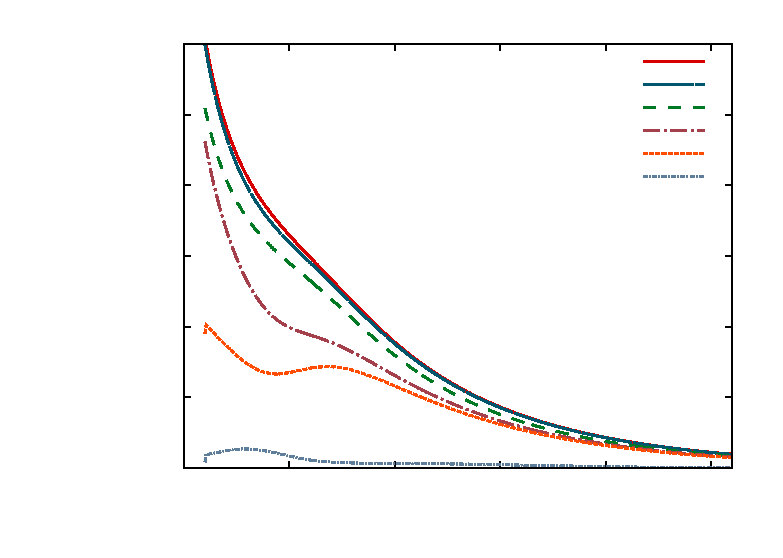
\includegraphics{img/PqdotNormsProjection}}%
    \gplfronttext
  \end{picture}%
\endgroup

    }
\end{center}
\caption{Evolution of the norm of the motion after successively projecting the motion in the
	tasks null spaces.}
\label{fig:xp3Pqdot}
\end{figure}

\subsection{Experiment 2 : Distinction between two close motions}
\label{sec:distinc}
An interesting challenge in motion detection,
is to make the distinction between two motions
involving different tasks but that produces very similar joint trajectory.
Anthropomorphic algorithm would use the context to perform the disambiguation.
The work presented in this paper shows that the fitting criteria
are sufficient to disambiguate similar looking motion.

\subsubsection{Reaching motions}
\label{sec:distinc1}
In this section, two motions are considered: \emph{motion 2.a} and \emph{motion 2.b}.
The first one is a far-reaching task motion with the right hand.
The reaching motion of the right hand has an influence on the left hand through the \emph{Com} task.
The second motion is the same reaching task motion for the right hand, added with a
second reaching task on the left hand. The desired position of the left
hand is artificially set to the final position of the left hand obtained at the first motion.

The final states of the robot for the two motions are showed in the Fig.~\ref{fig:introExample:spotDiff}.
A video showing those two motions on the HRP-2 is available\footnote{{http://homepages.laas.fr/shak/videos/}}.
The two motions look very similar, and it is very difficult
to tell which motion involves a left and right hand task without the context.
In the first case, the motion of the left hand is part of the \emph{com} task
motion, as it is a side effect to compensate the motion of the right hand.
In the second case, the motion of the left hand is independent,
because the left hand has been driven by its own goal.
However, in the proper task spaces, those motions are very different.
Fig.~\ref{fig:XP2RFit} shows the result of the task fitting for the \emph{motion 2.a}.
The residue (see equation~\ref{eq:residue}) of the optimization shows that the task fitting
performs poorly for the left hand task space
compared to the fitting on the right hand.
\begin{equation}
  r = \int{\frac{\Vert p^*(t) - p(t) \Vert^2}{\Vert p^*(t) \Vert^2} \mathrm{dt}} 
  \label{eq:residue}
\end{equation}
\begin{figure*}[t]
\centering
\begin{tabular*}{0.9\textwidth}{@{\extracolsep{\fill}}cc}
%\includegraphics[width=0.9\linewidth]{img/projRHNull.eps}
  \resizebox{.48\textwidth}{!} {
      % GNUPLOT: LaTeX picture with Postscript
\begingroup
  \makeatletter
  \providecommand\color[2][]{%
    \GenericError{(gnuplot) \space\space\space\@spaces}{%
      Package color not loaded in conjunction with
      terminal option `colourtext'%
    }{See the gnuplot documentation for explanation.%
    }{Either use 'blacktext' in gnuplot or load the package
      color.sty in LaTeX.}%
    \renewcommand\color[2][]{}%
  }%
  \providecommand\includegraphics[2][]{%
    \GenericError{(gnuplot) \space\space\space\@spaces}{%
      Package graphicx or graphics not loaded%
    }{See the gnuplot documentation for explanation.%
    }{The gnuplot epslatex terminal needs graphicx.sty or graphics.sty.}%
    \renewcommand\includegraphics[2][]{}%
  }%
  \providecommand\rotatebox[2]{#2}%
  \@ifundefined{ifGPcolor}{%
    \newif\ifGPcolor
    \GPcolortrue
  }{}%
  \@ifundefined{ifGPblacktext}{%
    \newif\ifGPblacktext
    \GPblacktexttrue
  }{}%
  % define a \g@addto@macro without @ in the name:
  \let\gplgaddtomacro\g@addto@macro
  % define empty templates for all commands taking text:
  \gdef\gplbacktext{}%
  \gdef\gplfronttext{}%
  \makeatother
  \ifGPblacktext
    % no textcolor at all
    \def\colorrgb#1{}%
    \def\colorgray#1{}%
  \else
    % gray or color?
    \ifGPcolor
      \def\colorrgb#1{\color[rgb]{#1}}%
      \def\colorgray#1{\color[gray]{#1}}%
      \expandafter\def\csname LTw\endcsname{\color{white}}%
      \expandafter\def\csname LTb\endcsname{\color{black}}%
      \expandafter\def\csname LTa\endcsname{\color{black}}%
      \expandafter\def\csname LT0\endcsname{\color[rgb]{1,0,0}}%
      \expandafter\def\csname LT1\endcsname{\color[rgb]{0,1,0}}%
      \expandafter\def\csname LT2\endcsname{\color[rgb]{0,0,1}}%
      \expandafter\def\csname LT3\endcsname{\color[rgb]{1,0,1}}%
      \expandafter\def\csname LT4\endcsname{\color[rgb]{0,1,1}}%
      \expandafter\def\csname LT5\endcsname{\color[rgb]{1,1,0}}%
      \expandafter\def\csname LT6\endcsname{\color[rgb]{0,0,0}}%
      \expandafter\def\csname LT7\endcsname{\color[rgb]{1,0.3,0}}%
      \expandafter\def\csname LT8\endcsname{\color[rgb]{0.5,0.5,0.5}}%
    \else
      % gray
      \def\colorrgb#1{\color{black}}%
      \def\colorgray#1{\color[gray]{#1}}%
      \expandafter\def\csname LTw\endcsname{\color{white}}%
      \expandafter\def\csname LTb\endcsname{\color{black}}%
      \expandafter\def\csname LTa\endcsname{\color{black}}%
      \expandafter\def\csname LT0\endcsname{\color{black}}%
      \expandafter\def\csname LT1\endcsname{\color{black}}%
      \expandafter\def\csname LT2\endcsname{\color{black}}%
      \expandafter\def\csname LT3\endcsname{\color{black}}%
      \expandafter\def\csname LT4\endcsname{\color{black}}%
      \expandafter\def\csname LT5\endcsname{\color{black}}%
      \expandafter\def\csname LT6\endcsname{\color{black}}%
      \expandafter\def\csname LT7\endcsname{\color{black}}%
      \expandafter\def\csname LT8\endcsname{\color{black}}%
    \fi
  \fi
  \setlength{\unitlength}{0.0500bp}%
  \begin{picture}(7200.00,5040.00)%
    \gplgaddtomacro\gplbacktext{%
      \csname LTb\endcsname%
      \put(990,704){\makebox(0,0)[r]{\strut{} 0}}%
      \put(990,1136){\makebox(0,0)[r]{\strut{} 0.2}}%
      \put(990,1569){\makebox(0,0)[r]{\strut{} 0.4}}%
      \put(990,2001){\makebox(0,0)[r]{\strut{} 0.6}}%
      \put(990,2434){\makebox(0,0)[r]{\strut{} 0.8}}%
      \put(990,2866){\makebox(0,0)[r]{\strut{} 1}}%
      \put(990,3299){\makebox(0,0)[r]{\strut{} 1.2}}%
      \put(990,3731){\makebox(0,0)[r]{\strut{} 1.4}}%
      \put(990,4164){\makebox(0,0)[r]{\strut{} 1.6}}%
      \put(1122,484){\makebox(0,0){\strut{} 0}}%
      \put(1937,484){\makebox(0,0){\strut{} 0.5}}%
      \put(2753,484){\makebox(0,0){\strut{} 1}}%
      \put(3568,484){\makebox(0,0){\strut{} 1.5}}%
      \put(4383,484){\makebox(0,0){\strut{} 2}}%
      \put(5199,484){\makebox(0,0){\strut{} 2.5}}%
      \put(6014,484){\makebox(0,0){\strut{} 3}}%
      \put(6829,484){\makebox(0,0){\strut{} 3.5}}%
      \put(3996,154){\makebox(0,0){\strut{}$t$ (s)}}%
      \put(3996,4710){\makebox(0,0){\strut{}$\begin{array}{rl} r &= 0.147227\\ \int \Vert \mathbf{J}^+ \mathbf{\dot{e}}_{taskRhand} \Vert \mathrm{d}t &=  0.40304 \mathrm{rad}\\ \end{array}$}}%
    }%
    \gplgaddtomacro\gplfronttext{%
      \csname LTb\endcsname%
      \put(5883,4207){\makebox(0,0)[r]{\strut{}$\Vert \mathbf{J}^+ \mathbf{\dot{e}}_{taskRhand} \Vert / \int \Vert \mathbf{J}^+ \mathbf{\dot{e}}_{taskRhand} \Vert \mathrm{d}t$}}%
      \csname LTb\endcsname%
      \put(5883,3987){\makebox(0,0)[r]{\strut{}Model}}%
    }%
    \gplbacktext
    \put(0,0){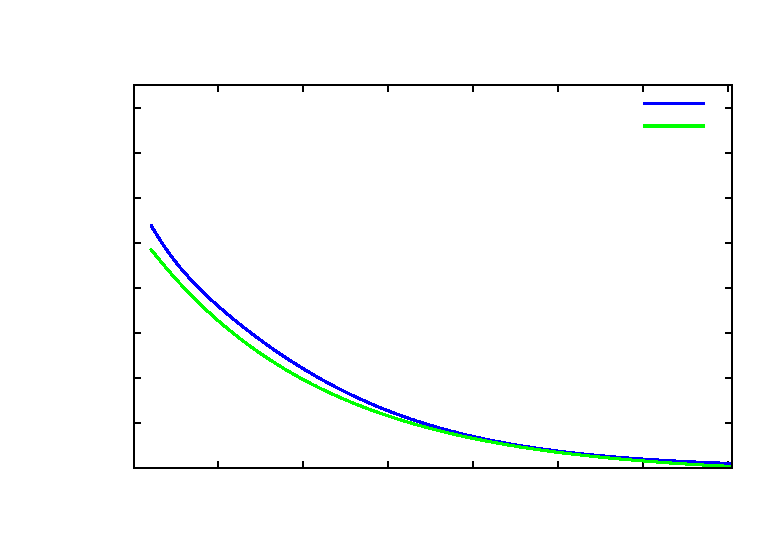
\includegraphics{img/simu/2a/taskRhandNormInvJerr_0}}%
    \gplfronttext
  \end{picture}%
\endgroup

    }          &
  \resizebox{.48\textwidth}{!} {
      % GNUPLOT: LaTeX picture with Postscript
\begingroup
  \makeatletter
  \providecommand\color[2][]{%
    \GenericError{(gnuplot) \space\space\space\@spaces}{%
      Package color not loaded in conjunction with
      terminal option `colourtext'%
    }{See the gnuplot documentation for explanation.%
    }{Either use 'blacktext' in gnuplot or load the package
      color.sty in LaTeX.}%
    \renewcommand\color[2][]{}%
  }%
  \providecommand\includegraphics[2][]{%
    \GenericError{(gnuplot) \space\space\space\@spaces}{%
      Package graphicx or graphics not loaded%
    }{See the gnuplot documentation for explanation.%
    }{The gnuplot epslatex terminal needs graphicx.sty or graphics.sty.}%
    \renewcommand\includegraphics[2][]{}%
  }%
  \providecommand\rotatebox[2]{#2}%
  \@ifundefined{ifGPcolor}{%
    \newif\ifGPcolor
    \GPcolortrue
  }{}%
  \@ifundefined{ifGPblacktext}{%
    \newif\ifGPblacktext
    \GPblacktexttrue
  }{}%
  % define a \g@addto@macro without @ in the name:
  \let\gplgaddtomacro\g@addto@macro
  % define empty templates for all commands taking text:
  \gdef\gplbacktext{}%
  \gdef\gplfronttext{}%
  \makeatother
  \ifGPblacktext
    % no textcolor at all
    \def\colorrgb#1{}%
    \def\colorgray#1{}%
  \else
    % gray or color?
    \ifGPcolor
      \def\colorrgb#1{\color[rgb]{#1}}%
      \def\colorgray#1{\color[gray]{#1}}%
      \expandafter\def\csname LTw\endcsname{\color{white}}%
      \expandafter\def\csname LTb\endcsname{\color{black}}%
      \expandafter\def\csname LTa\endcsname{\color{black}}%
      \expandafter\def\csname LT0\endcsname{\color[rgb]{1,0,0}}%
      \expandafter\def\csname LT1\endcsname{\color[rgb]{0,1,0}}%
      \expandafter\def\csname LT2\endcsname{\color[rgb]{0,0,1}}%
      \expandafter\def\csname LT3\endcsname{\color[rgb]{1,0,1}}%
      \expandafter\def\csname LT4\endcsname{\color[rgb]{0,1,1}}%
      \expandafter\def\csname LT5\endcsname{\color[rgb]{1,1,0}}%
      \expandafter\def\csname LT6\endcsname{\color[rgb]{0,0,0}}%
      \expandafter\def\csname LT7\endcsname{\color[rgb]{1,0.3,0}}%
      \expandafter\def\csname LT8\endcsname{\color[rgb]{0.5,0.5,0.5}}%
    \else
      % gray
      \def\colorrgb#1{\color{black}}%
      \def\colorgray#1{\color[gray]{#1}}%
      \expandafter\def\csname LTw\endcsname{\color{white}}%
      \expandafter\def\csname LTb\endcsname{\color{black}}%
      \expandafter\def\csname LTa\endcsname{\color{black}}%
      \expandafter\def\csname LT0\endcsname{\color{black}}%
      \expandafter\def\csname LT1\endcsname{\color{black}}%
      \expandafter\def\csname LT2\endcsname{\color{black}}%
      \expandafter\def\csname LT3\endcsname{\color{black}}%
      \expandafter\def\csname LT4\endcsname{\color{black}}%
      \expandafter\def\csname LT5\endcsname{\color{black}}%
      \expandafter\def\csname LT6\endcsname{\color{black}}%
      \expandafter\def\csname LT7\endcsname{\color{black}}%
      \expandafter\def\csname LT8\endcsname{\color{black}}%
    \fi
  \fi
  \setlength{\unitlength}{0.0500bp}%
  \begin{picture}(7200.00,5040.00)%
    \gplgaddtomacro\gplbacktext{%
      \csname LTb\endcsname%
      \put(990,704){\makebox(0,0)[r]{\strut{} 0}}%
      \put(990,1136){\makebox(0,0)[r]{\strut{} 0.2}}%
      \put(990,1569){\makebox(0,0)[r]{\strut{} 0.4}}%
      \put(990,2001){\makebox(0,0)[r]{\strut{} 0.6}}%
      \put(990,2434){\makebox(0,0)[r]{\strut{} 0.8}}%
      \put(990,2866){\makebox(0,0)[r]{\strut{} 1}}%
      \put(990,3299){\makebox(0,0)[r]{\strut{} 1.2}}%
      \put(990,3731){\makebox(0,0)[r]{\strut{} 1.4}}%
      \put(990,4164){\makebox(0,0)[r]{\strut{} 1.6}}%
      \put(1122,484){\makebox(0,0){\strut{} 0}}%
      \put(1937,484){\makebox(0,0){\strut{} 0.5}}%
      \put(2753,484){\makebox(0,0){\strut{} 1}}%
      \put(3568,484){\makebox(0,0){\strut{} 1.5}}%
      \put(4383,484){\makebox(0,0){\strut{} 2}}%
      \put(5199,484){\makebox(0,0){\strut{} 2.5}}%
      \put(6014,484){\makebox(0,0){\strut{} 3}}%
      \put(6829,484){\makebox(0,0){\strut{} 3.5}}%
      \put(3996,154){\makebox(0,0){\strut{}$t$ (s)}}%
      \put(3996,4710){\makebox(0,0){\strut{}$\begin{array}{rl} r &= 2.61576\\ \int \Vert \mathbf{J}^+ \mathbf{\dot{e}}_{taskLhand} \Vert \mathrm{d}t &=  0.189581 \mathrm{rad}\\ \end{array}$}}%
    }%
    \gplgaddtomacro\gplfronttext{%
      \csname LTb\endcsname%
      \put(5883,4207){\makebox(0,0)[r]{\strut{}$\Vert \mathbf{J}^+ \mathbf{\dot{e}}_{taskLhand} \Vert / \int \Vert \mathbf{J}^+ \mathbf{\dot{e}}_{taskLhand} \Vert \mathrm{d}t$}}%
      \csname LTb\endcsname%
      \put(5883,3987){\makebox(0,0)[r]{\strut{}Model}}%
    }%
    \gplbacktext
    \put(0,0){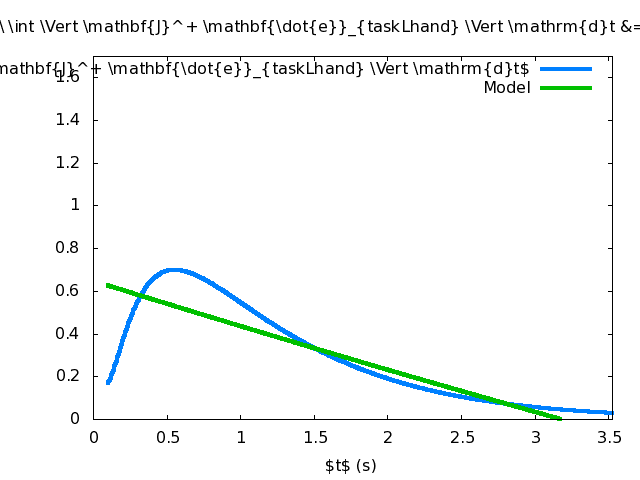
\includegraphics{img/simu/2a/taskLhandNormInvJerr_0}}%
    \gplfronttext
  \end{picture}%
\endgroup

    }\\
\end{tabular*}
\caption{Task fitting on the \emph{motion 2.a} on the right and the left hand tasks.}
\label{fig:XP2RFit}
\end{figure*}
Whereas Fig.~\ref{fig:XP2RLFit} shows the task fitting for the \emph{motion 2.b}.
\begin{figure*}[t]
\centering
\begin{tabular*}{0.9\textwidth}{@{\extracolsep{\fill}}cc}
%\includegraphics[width=0.9\linewidth]{img/projRHNull.eps}
  \resizebox{.48\textwidth}{!} {
      % GNUPLOT: LaTeX picture with Postscript
\begingroup
  \makeatletter
  \providecommand\color[2][]{%
    \GenericError{(gnuplot) \space\space\space\@spaces}{%
      Package color not loaded in conjunction with
      terminal option `colourtext'%
    }{See the gnuplot documentation for explanation.%
    }{Either use 'blacktext' in gnuplot or load the package
      color.sty in LaTeX.}%
    \renewcommand\color[2][]{}%
  }%
  \providecommand\includegraphics[2][]{%
    \GenericError{(gnuplot) \space\space\space\@spaces}{%
      Package graphicx or graphics not loaded%
    }{See the gnuplot documentation for explanation.%
    }{The gnuplot epslatex terminal needs graphicx.sty or graphics.sty.}%
    \renewcommand\includegraphics[2][]{}%
  }%
  \providecommand\rotatebox[2]{#2}%
  \@ifundefined{ifGPcolor}{%
    \newif\ifGPcolor
    \GPcolortrue
  }{}%
  \@ifundefined{ifGPblacktext}{%
    \newif\ifGPblacktext
    \GPblacktexttrue
  }{}%
  % define a \g@addto@macro without @ in the name:
  \let\gplgaddtomacro\g@addto@macro
  % define empty templates for all commands taking text:
  \gdef\gplbacktext{}%
  \gdef\gplfronttext{}%
  \makeatother
  \ifGPblacktext
    % no textcolor at all
    \def\colorrgb#1{}%
    \def\colorgray#1{}%
  \else
    % gray or color?
    \ifGPcolor
      \def\colorrgb#1{\color[rgb]{#1}}%
      \def\colorgray#1{\color[gray]{#1}}%
      \expandafter\def\csname LTw\endcsname{\color{white}}%
      \expandafter\def\csname LTb\endcsname{\color{black}}%
      \expandafter\def\csname LTa\endcsname{\color{black}}%
      \expandafter\def\csname LT0\endcsname{\color[rgb]{1,0,0}}%
      \expandafter\def\csname LT1\endcsname{\color[rgb]{0,1,0}}%
      \expandafter\def\csname LT2\endcsname{\color[rgb]{0,0,1}}%
      \expandafter\def\csname LT3\endcsname{\color[rgb]{1,0,1}}%
      \expandafter\def\csname LT4\endcsname{\color[rgb]{0,1,1}}%
      \expandafter\def\csname LT5\endcsname{\color[rgb]{1,1,0}}%
      \expandafter\def\csname LT6\endcsname{\color[rgb]{0,0,0}}%
      \expandafter\def\csname LT7\endcsname{\color[rgb]{1,0.3,0}}%
      \expandafter\def\csname LT8\endcsname{\color[rgb]{0.5,0.5,0.5}}%
    \else
      % gray
      \def\colorrgb#1{\color{black}}%
      \def\colorgray#1{\color[gray]{#1}}%
      \expandafter\def\csname LTw\endcsname{\color{white}}%
      \expandafter\def\csname LTb\endcsname{\color{black}}%
      \expandafter\def\csname LTa\endcsname{\color{black}}%
      \expandafter\def\csname LT0\endcsname{\color{black}}%
      \expandafter\def\csname LT1\endcsname{\color{black}}%
      \expandafter\def\csname LT2\endcsname{\color{black}}%
      \expandafter\def\csname LT3\endcsname{\color{black}}%
      \expandafter\def\csname LT4\endcsname{\color{black}}%
      \expandafter\def\csname LT5\endcsname{\color{black}}%
      \expandafter\def\csname LT6\endcsname{\color{black}}%
      \expandafter\def\csname LT7\endcsname{\color{black}}%
      \expandafter\def\csname LT8\endcsname{\color{black}}%
    \fi
  \fi
  \setlength{\unitlength}{0.0500bp}%
  \begin{picture}(7200.00,5040.00)%
    \gplgaddtomacro\gplbacktext{%
      \csname LTb\endcsname%
      \put(990,704){\makebox(0,0)[r]{\strut{} 0}}%
      \put(990,1136){\makebox(0,0)[r]{\strut{} 0.2}}%
      \put(990,1569){\makebox(0,0)[r]{\strut{} 0.4}}%
      \put(990,2001){\makebox(0,0)[r]{\strut{} 0.6}}%
      \put(990,2434){\makebox(0,0)[r]{\strut{} 0.8}}%
      \put(990,2866){\makebox(0,0)[r]{\strut{} 1}}%
      \put(990,3299){\makebox(0,0)[r]{\strut{} 1.2}}%
      \put(990,3731){\makebox(0,0)[r]{\strut{} 1.4}}%
      \put(990,4164){\makebox(0,0)[r]{\strut{} 1.6}}%
      \put(1122,484){\makebox(0,0){\strut{} 0}}%
      \put(1937,484){\makebox(0,0){\strut{} 0.5}}%
      \put(2753,484){\makebox(0,0){\strut{} 1}}%
      \put(3568,484){\makebox(0,0){\strut{} 1.5}}%
      \put(4383,484){\makebox(0,0){\strut{} 2}}%
      \put(5199,484){\makebox(0,0){\strut{} 2.5}}%
      \put(6014,484){\makebox(0,0){\strut{} 3}}%
      \put(6829,484){\makebox(0,0){\strut{} 3.5}}%
      \put(3996,154){\makebox(0,0){\strut{}$t$ (s)}}%
      \put(3996,4710){\makebox(0,0){\strut{}$\begin{array}{rl} r &= 0.186639\\ \int \Vert \mathbf{J}^+ \mathbf{\dot{e}}_{taskRhand} \Vert \mathrm{d}t &=  0.403712 \mathrm{rad}\\ \end{array}$}}%
    }%
    \gplgaddtomacro\gplfronttext{%
      \csname LTb\endcsname%
      \put(5883,4207){\makebox(0,0)[r]{\strut{}$\Vert \mathbf{J}^+ \mathbf{\dot{e}}_{taskRhand} \Vert / \int \Vert \mathbf{J}^+ \mathbf{\dot{e}}_{taskRhand} \Vert \mathrm{d}t$}}%
      \csname LTb\endcsname%
      \put(5883,3987){\makebox(0,0)[r]{\strut{}Model}}%
    }%
    \gplbacktext
    \put(0,0){\includegraphics{img/simu/2b/taskRhandNormInvJerr_0}}%
    \gplfronttext
  \end{picture}%
\endgroup

    }                           &
  \resizebox{.48\textwidth}{!} {
      % GNUPLOT: LaTeX picture with Postscript
\begingroup
  \makeatletter
  \providecommand\color[2][]{%
    \GenericError{(gnuplot) \space\space\space\@spaces}{%
      Package color not loaded in conjunction with
      terminal option `colourtext'%
    }{See the gnuplot documentation for explanation.%
    }{Either use 'blacktext' in gnuplot or load the package
      color.sty in LaTeX.}%
    \renewcommand\color[2][]{}%
  }%
  \providecommand\includegraphics[2][]{%
    \GenericError{(gnuplot) \space\space\space\@spaces}{%
      Package graphicx or graphics not loaded%
    }{See the gnuplot documentation for explanation.%
    }{The gnuplot epslatex terminal needs graphicx.sty or graphics.sty.}%
    \renewcommand\includegraphics[2][]{}%
  }%
  \providecommand\rotatebox[2]{#2}%
  \@ifundefined{ifGPcolor}{%
    \newif\ifGPcolor
    \GPcolortrue
  }{}%
  \@ifundefined{ifGPblacktext}{%
    \newif\ifGPblacktext
    \GPblacktexttrue
  }{}%
  % define a \g@addto@macro without @ in the name:
  \let\gplgaddtomacro\g@addto@macro
  % define empty templates for all commands taking text:
  \gdef\gplbacktext{}%
  \gdef\gplfronttext{}%
  \makeatother
  \ifGPblacktext
    % no textcolor at all
    \def\colorrgb#1{}%
    \def\colorgray#1{}%
  \else
    % gray or color?
    \ifGPcolor
      \def\colorrgb#1{\color[rgb]{#1}}%
      \def\colorgray#1{\color[gray]{#1}}%
      \expandafter\def\csname LTw\endcsname{\color{white}}%
      \expandafter\def\csname LTb\endcsname{\color{black}}%
      \expandafter\def\csname LTa\endcsname{\color{black}}%
      \expandafter\def\csname LT0\endcsname{\color[rgb]{1,0,0}}%
      \expandafter\def\csname LT1\endcsname{\color[rgb]{0,1,0}}%
      \expandafter\def\csname LT2\endcsname{\color[rgb]{0,0,1}}%
      \expandafter\def\csname LT3\endcsname{\color[rgb]{1,0,1}}%
      \expandafter\def\csname LT4\endcsname{\color[rgb]{0,1,1}}%
      \expandafter\def\csname LT5\endcsname{\color[rgb]{1,1,0}}%
      \expandafter\def\csname LT6\endcsname{\color[rgb]{0,0,0}}%
      \expandafter\def\csname LT7\endcsname{\color[rgb]{1,0.3,0}}%
      \expandafter\def\csname LT8\endcsname{\color[rgb]{0.5,0.5,0.5}}%
    \else
      % gray
      \def\colorrgb#1{\color{black}}%
      \def\colorgray#1{\color[gray]{#1}}%
      \expandafter\def\csname LTw\endcsname{\color{white}}%
      \expandafter\def\csname LTb\endcsname{\color{black}}%
      \expandafter\def\csname LTa\endcsname{\color{black}}%
      \expandafter\def\csname LT0\endcsname{\color{black}}%
      \expandafter\def\csname LT1\endcsname{\color{black}}%
      \expandafter\def\csname LT2\endcsname{\color{black}}%
      \expandafter\def\csname LT3\endcsname{\color{black}}%
      \expandafter\def\csname LT4\endcsname{\color{black}}%
      \expandafter\def\csname LT5\endcsname{\color{black}}%
      \expandafter\def\csname LT6\endcsname{\color{black}}%
      \expandafter\def\csname LT7\endcsname{\color{black}}%
      \expandafter\def\csname LT8\endcsname{\color{black}}%
    \fi
  \fi
  \setlength{\unitlength}{0.0500bp}%
  \begin{picture}(7200.00,5040.00)%
    \gplgaddtomacro\gplbacktext{%
      \csname LTb\endcsname%
      \put(990,704){\makebox(0,0)[r]{\strut{} 0}}%
      \put(990,1136){\makebox(0,0)[r]{\strut{} 0.2}}%
      \put(990,1569){\makebox(0,0)[r]{\strut{} 0.4}}%
      \put(990,2001){\makebox(0,0)[r]{\strut{} 0.6}}%
      \put(990,2434){\makebox(0,0)[r]{\strut{} 0.8}}%
      \put(990,2866){\makebox(0,0)[r]{\strut{} 1}}%
      \put(990,3299){\makebox(0,0)[r]{\strut{} 1.2}}%
      \put(990,3731){\makebox(0,0)[r]{\strut{} 1.4}}%
      \put(990,4164){\makebox(0,0)[r]{\strut{} 1.6}}%
      \put(1122,484){\makebox(0,0){\strut{} 0}}%
      \put(1937,484){\makebox(0,0){\strut{} 0.5}}%
      \put(2753,484){\makebox(0,0){\strut{} 1}}%
      \put(3568,484){\makebox(0,0){\strut{} 1.5}}%
      \put(4383,484){\makebox(0,0){\strut{} 2}}%
      \put(5199,484){\makebox(0,0){\strut{} 2.5}}%
      \put(6014,484){\makebox(0,0){\strut{} 3}}%
      \put(6829,484){\makebox(0,0){\strut{} 3.5}}%
      \put(3996,154){\makebox(0,0){\strut{}$t$ (s)}}%
      \put(3996,4710){\makebox(0,0){\strut{}$\begin{array}{rl} r &= 0.301578\\ \int \Vert \mathbf{J}^+ \mathbf{\dot{e}}_{taskLhand} \Vert \mathrm{d}t &=  0.187033 \mathrm{rad}\\ \end{array}$}}%
    }%
    \gplgaddtomacro\gplfronttext{%
      \csname LTb\endcsname%
      \put(5883,4207){\makebox(0,0)[r]{\strut{}$\Vert \mathbf{J}^+ \mathbf{\dot{e}}_{taskLhand} \Vert / \int \Vert \mathbf{J}^+ \mathbf{\dot{e}}_{taskLhand} \Vert \mathrm{d}t$}}%
      \csname LTb\endcsname%
      \put(5883,3987){\makebox(0,0)[r]{\strut{}Model}}%
    }%
    \gplbacktext
    \put(0,0){\includegraphics{img/simu/2b/taskLhandNormInvJerr_0}}%
    \gplfronttext
  \end{picture}%
\endgroup

    }\\
\end{tabular*}
\caption{Task fitting on the \emph{motion 2.b} on the right and the left hand tasks.}
\label{fig:XP2RLFit}
\end{figure*}
The results of the detection algorithm
applied to those motion are showed in Table~\ref{tab:spotDiff1}.
\begin{table}[t]
\centering
\begin{tabular}{|c|c|c|c|}
\hline
Reference & Detected & $\int \Vert \dot{q}(t) \Vert ^2 dt$ & $\int \Vert P\dot{q}(t) \Vert ^2 dt$ \\
\hline
\begin{tabular}{c}
Com\\
Right Hand\\
Twofeet\\
\end{tabular}

&

\begin{tabular}{c}
Com\\
Right Hand\\
Twofeet\\
\end{tabular}

& 0.364398 & 0.00159355 \\
\hline
\begin{tabular}{c}
Com\\
Left Hand\\
Right Hand\\
Twofeet\\
\end{tabular}

&
\begin{tabular}{c}
Com\\
Left Hand\\
Right Hand\\
Twofeet\\
\end{tabular}

& 0.538329  & 0.0035343 \\
\hline
\end{tabular}
\caption{Results of the task selection algorithm from the analysis of the \emph{motion 2.a} and the \emph{motion 2.b}.}
\label{tab:spotDiff1}
\vspace{-20pt}
\end{table}
The first column shows the
tasks being used in the reference motion, the second columns shows the tasks
selected by the algorithm, the third column shows the norm of the reference motion,
and the last column shows the norm of the reference motion projected onto the null space of
all the selected tasks. The threshold for the stop criterion $\int \Vert P\dot{q}(t) \Vert ^2 dt > \epsilon$
is $\epsilon = 0.1$.
The projection of the motion in the null space of the \emph{right grab} and \emph{com} task
will have different consequences for the \emph{motion 2.a} and \emph{motion 2.b}.
Fig.~\ref{fig:RbeforeAfterProj} shows how the norm of the joint angles velocities relevants to the tasks
\emph{right grab} and \emph{left grab} evolve after the projection of the motion.
Projecting the \emph{motion 2.a} into the null spaces of
the \emph{right grab} task will decrease its associated theoritical joint angles velocities while leaving the
\emph{left grab} one unchanged. Fig.~\ref{fig:RbeforeAfterProj} shows
that the theoretical joint angles velocities associated to the
\emph{left grab} task is decreased after the projection of the motion in
the nullspace of the \emph{com} task.  That means that
the left arm of the robot was controlled by the \emph{com} task.

On the other hand, when projecting the \emph{motion 2.b} into the nullspace of the \emph{right grab}
and \emph{com} task the joint angle velocities associated to the \emph{left grab} task
is still significant. That means that the \emph{com} task has a little influence on the
motion of the left arm. Therefore, the task selection algorithm will still look
for the task that has controlled the left arm.

It has to be noted that the norm of the last joint angles velocities are not null, because 
the task selection algorithm has not finished and other tasks have not been selected yet.
\begin{figure*}[t]
\centering
  \subfigure[Motion 2.a]{
  \resizebox{.48\textwidth}{!} {
      % GNUPLOT: LaTeX picture with Postscript
\begingroup
  \makeatletter
  \providecommand\color[2][]{%
    \GenericError{(gnuplot) \space\space\space\@spaces}{%
      Package color not loaded in conjunction with
      terminal option `colourtext'%
    }{See the gnuplot documentation for explanation.%
    }{Either use 'blacktext' in gnuplot or load the package
      color.sty in LaTeX.}%
    \renewcommand\color[2][]{}%
  }%
  \providecommand\includegraphics[2][]{%
    \GenericError{(gnuplot) \space\space\space\@spaces}{%
      Package graphicx or graphics not loaded%
    }{See the gnuplot documentation for explanation.%
    }{The gnuplot epslatex terminal needs graphicx.sty or graphics.sty.}%
    \renewcommand\includegraphics[2][]{}%
  }%
  \providecommand\rotatebox[2]{#2}%
  \@ifundefined{ifGPcolor}{%
    \newif\ifGPcolor
    \GPcolortrue
  }{}%
  \@ifundefined{ifGPblacktext}{%
    \newif\ifGPblacktext
    \GPblacktexttrue
  }{}%
  % define a \g@addto@macro without @ in the name:
  \let\gplgaddtomacro\g@addto@macro
  % define empty templates for all commands taking text:
  \gdef\gplbacktext{}%
  \gdef\gplfronttext{}%
  \makeatother
  \ifGPblacktext
    % no textcolor at all
    \def\colorrgb#1{}%
    \def\colorgray#1{}%
  \else
    % gray or color?
    \ifGPcolor
      \def\colorrgb#1{\color[rgb]{#1}}%
      \def\colorgray#1{\color[gray]{#1}}%
      \expandafter\def\csname LTw\endcsname{\color{white}}%
      \expandafter\def\csname LTb\endcsname{\color{black}}%
      \expandafter\def\csname LTa\endcsname{\color{black}}%
      \expandafter\def\csname LT0\endcsname{\color[rgb]{1,0,0}}%
      \expandafter\def\csname LT1\endcsname{\color[rgb]{0,1,0}}%
      \expandafter\def\csname LT2\endcsname{\color[rgb]{0,0,1}}%
      \expandafter\def\csname LT3\endcsname{\color[rgb]{1,0,1}}%
      \expandafter\def\csname LT4\endcsname{\color[rgb]{0,1,1}}%
      \expandafter\def\csname LT5\endcsname{\color[rgb]{1,1,0}}%
      \expandafter\def\csname LT6\endcsname{\color[rgb]{0,0,0}}%
      \expandafter\def\csname LT7\endcsname{\color[rgb]{1,0.3,0}}%
      \expandafter\def\csname LT8\endcsname{\color[rgb]{0.5,0.5,0.5}}%
    \else
      % gray
      \def\colorrgb#1{\color{black}}%
      \def\colorgray#1{\color[gray]{#1}}%
      \expandafter\def\csname LTw\endcsname{\color{white}}%
      \expandafter\def\csname LTb\endcsname{\color{black}}%
      \expandafter\def\csname LTa\endcsname{\color{black}}%
      \expandafter\def\csname LT0\endcsname{\color{black}}%
      \expandafter\def\csname LT1\endcsname{\color{black}}%
      \expandafter\def\csname LT2\endcsname{\color{black}}%
      \expandafter\def\csname LT3\endcsname{\color{black}}%
      \expandafter\def\csname LT4\endcsname{\color{black}}%
      \expandafter\def\csname LT5\endcsname{\color{black}}%
      \expandafter\def\csname LT6\endcsname{\color{black}}%
      \expandafter\def\csname LT7\endcsname{\color{black}}%
      \expandafter\def\csname LT8\endcsname{\color{black}}%
    \fi
  \fi
  \setlength{\unitlength}{0.0500bp}%
  \begin{picture}(7200.00,5040.00)%
    \gplgaddtomacro\gplbacktext{%
      \csname LTb\endcsname%
      \put(1342,704){\makebox(0,0)[r]{\strut{} 0}}%
      \put(1342,1156){\makebox(0,0)[r]{\strut{} 0.05}}%
      \put(1342,1609){\makebox(0,0)[r]{\strut{} 0.1}}%
      \put(1342,2061){\makebox(0,0)[r]{\strut{} 0.15}}%
      \put(1342,2514){\makebox(0,0)[r]{\strut{} 0.2}}%
      \put(1342,2966){\makebox(0,0)[r]{\strut{} 0.25}}%
      \put(1342,3419){\makebox(0,0)[r]{\strut{} 0.3}}%
      \put(1342,3871){\makebox(0,0)[r]{\strut{} 0.35}}%
      \put(1342,4324){\makebox(0,0)[r]{\strut{} 0.4}}%
      \put(1342,4776){\makebox(0,0)[r]{\strut{} 0.45}}%
      \put(1474,484){\makebox(0,0){\strut{} 0}}%
      \put(2235,484){\makebox(0,0){\strut{} 0.5}}%
      \put(2996,484){\makebox(0,0){\strut{} 1}}%
      \put(3757,484){\makebox(0,0){\strut{} 1.5}}%
      \put(4518,484){\makebox(0,0){\strut{} 2}}%
      \put(5279,484){\makebox(0,0){\strut{} 2.5}}%
      \put(6040,484){\makebox(0,0){\strut{} 3}}%
      \put(6802,484){\makebox(0,0){\strut{} 3.5}}%
      \put(440,2740){\rotatebox{90}{\makebox(0,0){\strut{}$\Vert \mathbf{\dot{q}} \Vert$ (rad/s)}}}%
      \put(4172,154){\makebox(0,0){\strut{}$t$ (s)}}%
    }%
    \gplgaddtomacro\gplfronttext{%
      \csname LTb\endcsname%
      \put(5883,4603){\makebox(0,0)[r]{\strut{}$\Vert \mathbf{J}_{rhand}^+\mathbf{J}_{rhand} \mathbf{\dot{q}} \Vert$}}%
      \csname LTb\endcsname%
      \put(5883,4383){\makebox(0,0)[r]{\strut{}$\Vert \mathbf{J}_{rhand}^+\mathbf{J}_{rhand} \mathbf{P}_{rhand} \mathbf{\dot{q}} \Vert$}}%
      \csname LTb\endcsname%
      \put(5883,4163){\makebox(0,0)[r]{\strut{}$\Vert \mathbf{J}_{rhand}^+\mathbf{J}_{rhand} \mathbf{P}_{rhand+com} \mathbf{\dot{q}} \Vert$}}%
      \csname LTb\endcsname%
      \put(5883,3943){\makebox(0,0)[r]{\strut{}$\Vert \mathbf{J}_{lhand}^+\mathbf{J}_{lhand} \mathbf{\dot{q}} \Vert$}}%
      \csname LTb\endcsname%
      \put(5883,3723){\makebox(0,0)[r]{\strut{}$\Vert \mathbf{J}_{lhand}^+\mathbf{J}_{lhand} \mathbf{P}_{rhand} \mathbf{\dot{q}} \Vert$}}%
      \csname LTb\endcsname%
      \put(5883,3503){\makebox(0,0)[r]{\strut{}$\Vert \mathbf{J}_{lhand}^+\mathbf{J}_{lhand} \mathbf{P}_{rhand+com} \mathbf{\dot{q}} \Vert$}}%
    }%
    \gplbacktext
    \put(0,0){\includegraphics{img/simu/2a/RbeforeAfterProj}}%
    \gplfronttext
  \end{picture}%
\endgroup

    }
  \label{fig:RbeforeAfterProj:2a}
  }
  \subfigure[Motion 2.b]{
  \resizebox{.48\textwidth}{!} {
      % GNUPLOT: LaTeX picture with Postscript
\begingroup
  \makeatletter
  \providecommand\color[2][]{%
    \GenericError{(gnuplot) \space\space\space\@spaces}{%
      Package color not loaded in conjunction with
      terminal option `colourtext'%
    }{See the gnuplot documentation for explanation.%
    }{Either use 'blacktext' in gnuplot or load the package
      color.sty in LaTeX.}%
    \renewcommand\color[2][]{}%
  }%
  \providecommand\includegraphics[2][]{%
    \GenericError{(gnuplot) \space\space\space\@spaces}{%
      Package graphicx or graphics not loaded%
    }{See the gnuplot documentation for explanation.%
    }{The gnuplot epslatex terminal needs graphicx.sty or graphics.sty.}%
    \renewcommand\includegraphics[2][]{}%
  }%
  \providecommand\rotatebox[2]{#2}%
  \@ifundefined{ifGPcolor}{%
    \newif\ifGPcolor
    \GPcolortrue
  }{}%
  \@ifundefined{ifGPblacktext}{%
    \newif\ifGPblacktext
    \GPblacktexttrue
  }{}%
  % define a \g@addto@macro without @ in the name:
  \let\gplgaddtomacro\g@addto@macro
  % define empty templates for all commands taking text:
  \gdef\gplbacktext{}%
  \gdef\gplfronttext{}%
  \makeatother
  \ifGPblacktext
    % no textcolor at all
    \def\colorrgb#1{}%
    \def\colorgray#1{}%
  \else
    % gray or color?
    \ifGPcolor
      \def\colorrgb#1{\color[rgb]{#1}}%
      \def\colorgray#1{\color[gray]{#1}}%
      \expandafter\def\csname LTw\endcsname{\color{white}}%
      \expandafter\def\csname LTb\endcsname{\color{black}}%
      \expandafter\def\csname LTa\endcsname{\color{black}}%
      \expandafter\def\csname LT0\endcsname{\color[rgb]{1,0,0}}%
      \expandafter\def\csname LT1\endcsname{\color[rgb]{0,1,0}}%
      \expandafter\def\csname LT2\endcsname{\color[rgb]{0,0,1}}%
      \expandafter\def\csname LT3\endcsname{\color[rgb]{1,0,1}}%
      \expandafter\def\csname LT4\endcsname{\color[rgb]{0,1,1}}%
      \expandafter\def\csname LT5\endcsname{\color[rgb]{1,1,0}}%
      \expandafter\def\csname LT6\endcsname{\color[rgb]{0,0,0}}%
      \expandafter\def\csname LT7\endcsname{\color[rgb]{1,0.3,0}}%
      \expandafter\def\csname LT8\endcsname{\color[rgb]{0.5,0.5,0.5}}%
    \else
      % gray
      \def\colorrgb#1{\color{black}}%
      \def\colorgray#1{\color[gray]{#1}}%
      \expandafter\def\csname LTw\endcsname{\color{white}}%
      \expandafter\def\csname LTb\endcsname{\color{black}}%
      \expandafter\def\csname LTa\endcsname{\color{black}}%
      \expandafter\def\csname LT0\endcsname{\color{black}}%
      \expandafter\def\csname LT1\endcsname{\color{black}}%
      \expandafter\def\csname LT2\endcsname{\color{black}}%
      \expandafter\def\csname LT3\endcsname{\color{black}}%
      \expandafter\def\csname LT4\endcsname{\color{black}}%
      \expandafter\def\csname LT5\endcsname{\color{black}}%
      \expandafter\def\csname LT6\endcsname{\color{black}}%
      \expandafter\def\csname LT7\endcsname{\color{black}}%
      \expandafter\def\csname LT8\endcsname{\color{black}}%
    \fi
  \fi
  \setlength{\unitlength}{0.0500bp}%
  \begin{picture}(7200.00,5040.00)%
    \gplgaddtomacro\gplbacktext{%
      \csname LTb\endcsname%
      \put(1342,704){\makebox(0,0)[r]{\strut{} 0}}%
      \put(1342,1156){\makebox(0,0)[r]{\strut{} 0.05}}%
      \put(1342,1609){\makebox(0,0)[r]{\strut{} 0.1}}%
      \put(1342,2061){\makebox(0,0)[r]{\strut{} 0.15}}%
      \put(1342,2514){\makebox(0,0)[r]{\strut{} 0.2}}%
      \put(1342,2966){\makebox(0,0)[r]{\strut{} 0.25}}%
      \put(1342,3419){\makebox(0,0)[r]{\strut{} 0.3}}%
      \put(1342,3871){\makebox(0,0)[r]{\strut{} 0.35}}%
      \put(1342,4324){\makebox(0,0)[r]{\strut{} 0.4}}%
      \put(1342,4776){\makebox(0,0)[r]{\strut{} 0.45}}%
      \put(1474,484){\makebox(0,0){\strut{} 0}}%
      \put(2235,484){\makebox(0,0){\strut{} 0.5}}%
      \put(2996,484){\makebox(0,0){\strut{} 1}}%
      \put(3757,484){\makebox(0,0){\strut{} 1.5}}%
      \put(4518,484){\makebox(0,0){\strut{} 2}}%
      \put(5279,484){\makebox(0,0){\strut{} 2.5}}%
      \put(6040,484){\makebox(0,0){\strut{} 3}}%
      \put(6802,484){\makebox(0,0){\strut{} 3.5}}%
      \put(440,2740){\rotatebox{90}{\makebox(0,0){\strut{}$\Vert \mathbf{\dot{q}} \Vert$ (rad/s)}}}%
      \put(4172,154){\makebox(0,0){\strut{}$t$ (s)}}%
    }%
    \gplgaddtomacro\gplfronttext{%
      \csname LTb\endcsname%
      \put(5883,4603){\makebox(0,0)[r]{\strut{}$\Vert \mathbf{J}_{rhand}^+\mathbf{J}_{rhand} \mathbf{\dot{q}} \Vert$}}%
      \csname LTb\endcsname%
      \put(5883,4383){\makebox(0,0)[r]{\strut{}$\Vert \mathbf{J}_{rhand}^+\mathbf{J}_{rhand} \mathbf{P}_{rhand} \mathbf{\dot{q}} \Vert$}}%
      \csname LTb\endcsname%
      \put(5883,4163){\makebox(0,0)[r]{\strut{}$\Vert \mathbf{J}_{rhand}^+\mathbf{J}_{rhand} \mathbf{P}_{rhand+com} \mathbf{\dot{q}} \Vert$}}%
      \csname LTb\endcsname%
      \put(5883,3943){\makebox(0,0)[r]{\strut{}$\Vert \mathbf{J}_{lhand}^+\mathbf{J}_{lhand} \mathbf{\dot{q}} \Vert$}}%
      \csname LTb\endcsname%
      \put(5883,3723){\makebox(0,0)[r]{\strut{}$\Vert \mathbf{J}_{lhand}^+\mathbf{J}_{lhand} \mathbf{P}_{rhand} \mathbf{\dot{q}} \Vert$}}%
      \csname LTb\endcsname%
      \put(5883,3503){\makebox(0,0)[r]{\strut{}$\Vert \mathbf{J}_{lhand}^+\mathbf{J}_{lhand} \mathbf{P}_{rhand+com} \mathbf{\dot{q}} \Vert$}}%
    }%
    \gplbacktext
    \put(0,0){\includegraphics{img/simu/2b/RbeforeAfterProj}}%
    \gplfronttext
  \end{picture}%
\endgroup

  }
  \label{fig:RbeforeAfterProj:2b}
  }
  \caption{Evolution of the commands relevant to the \emph{right grab} (from dark to light red) and 
  \emph{left grab} (from dark to light blue) tasks after
  successive projection of the motion in the nullspace of the task \emph{right grab} and in the nullspace
  of the task \emph{com}. In the motion 2.a, a great part of the motion of the left arm is due to the \emph{com} task.
  Removing the \emph{com} task will cancel almost all motion in the left arm.
  In the motion 2.b, the left arm the motion of the left arm is not only involved by the \emph{com} task
  but also by the \emph{left grab} task. Removing the \emph{com} task will only
  cancel a little part of the motion of the left arm.}
\label{fig:RbeforeAfterProj}
\end{figure*}

\subsubsection{Grabing VS Screwing}
\label{sec:distinc2}
In this section, the two motions considered are the \emph{motion 3.a} and \emph{motion 3.b}.
Both motions share the same position target. The only difference between
the two demonstrated motions is the
presence of an orientation constraint for the right hand in the \emph{motion 3.b}.
The final positions of those motions are showed in the Fig.~\ref{fig:spotDiff2}.
\begin{figure}[t]
\begin{center}
\includegraphics[width=0.55\linewidth]{img/spotDiff2bis.ps}
\end{center}
\caption{Left: The final position of the \emph{motion 3.a}; Right: The final position of the \emph{motion 3.b}.}
\label{fig:spotDiff2}
\vspace{-3pt}
\end{figure}
Table~\ref{tab:spotDiff2} shows the results of the tasks selection algorithm which performed successfully.
\begin{table}[t]
\centering
\begin{tabular}{|c|c|c|c|}
\hline
Reference & Detected & $\int \Vert \dot{q}(t) \Vert ^2 dt$ & $\int \Vert P\dot{q}(t) \Vert ^2 dt$ \\
\hline
\begin{tabular}{c}
Com\\
Gaze\\
Grab\\
Twofeet\\
\end{tabular}
&
\begin{tabular}{c}
Com\\
Gaze\\
Grab\\
Twofeet\\
\end{tabular}
& 0.838686 & 0.0132712 \\
\hline
\begin{tabular}{c}
Com\\
Gaze\\
Screw\\
Twofeet\\
\end{tabular}
&
\begin{tabular}{c}
Com\\
Gaze\\
Screw\\
Twofeet\\
\end{tabular}
& 1.23008 & 0.0170635\\
\hline
\end{tabular}
\caption{Results of the task selection algorithm from the analysis of the
\emph{motion 3.a} and the \emph{motion 3.b}.}
\label{tab:spotDiff2}
\vspace{-3pt}
\end{table}
%During the analysis of the \emph{motion 3.b}, the \emph{grabbing} task
%is selected as well since the grab task is
%actually a sub-task of the \emph{screwing} motion. Of course, the \emph{screwing} task is not selected
%in the analysis of the \emph{motion 3.a}.

\subsubsection{Screw VS Gaze}
\label{sec:distinc3}
The two motions considered are the \emph{motion 4.a} and \emph{motion 4.b}.
The \emph{motion 4.a} can be described by the following scenario :
an object is in front of the robot, and creates an occlusion in the vision of the robot.
To get rid of this occlusion, the robot can lean on his right. 
While the robots leans, the left hand is dragged by the chest.
The position and orientation of that hand is recorded as a desired state for the first \emph{motion 4.b} task.
The final states of the robot are showed in Fig.~\ref{fig:spotDiff3}
and the results of the analysis are summarized in Table~\ref{tab:spotDiff3}.
\begin{figure}[t]
\begin{center}
\includegraphics[width=0.66\linewidth]{img/spotDiff3.ps}
\end{center}
\caption{Left: The final position of the \emph{motion 4.a}; Right: The final position of the \emph{motion 4.b}.}
\label{fig:spotDiff3}
\end{figure}
\begin{table}[t]
\centering
\begin{tabular}{|c|c|c|c|}
\hline
Reference & Detected & $\int \Vert \dot{q}(t) \Vert ^2 dt$ & $\int \Vert P\dot{q}(t) \Vert ^2 dt$ \\
\hline
\begin{tabular}{c}
Com\\
Gaze\\
Twofeet\\
\end{tabular}

&

\begin{tabular}{c}
Com\\
Gaze\\
Twofeet\\
\end{tabular}

& 0.534478 & 0.0545944 \\
\hline
\begin{tabular}{c}
Com\\
Screw\\
Twofeet\\
\end{tabular}

&
\begin{tabular}{c}
Com\\
Screw\\
Twofeet\\
\end{tabular}

& 0.558084 & 0.0023297\\
\hline
\end{tabular}
\caption{Results of the task selection algorithm from the analysis of the \emph{motion 4.a} and the \emph{motion 4.b}.}
\label{tab:spotDiff3}
\vspace{-12pt}
\end{table}

\section{Experimentation on the robot}
\label{sec:real}
In this section, we will experimentally demonstrate the validity of the task recognition algorithm
in realistic situation in presence of noise by observing the reference motion on the
real HRP-2 using a motion capture system. The task recognition algorithm 
is applied to two set of similar looking motions.

\subsection{Experimental setup}
A motion generated with the \emph{SoT} is executed on the Robot HRP-2 and
a motion capture system provides the trajectory of each body of the robot.
The motion capture system used is composed of 10 digital cameras and record data
at 200Hz (see Fig.~\ref{fig:camera}). 
\begin{figure}[t]
  \centering
  \includegraphics[height=0.4\linewidth]{img/camIRTest.eps} 
  \caption{Camera of the motion capture system.}
  \label{fig:camera}
\end{figure}
A set of 50 markers
are placed on the robot (Fig.~\ref{fig:hrp2Markers}), and the data collected from those markers
are used to build a virtual skeleton that match the kinematic hierarchy of the robot.
\begin{figure}[t]
  \centering
  \begin{tabular}{cc}
    \includegraphics[height=0.7\linewidth]{img/hrp2Markers.ps} &
    \includegraphics[height=0.7\linewidth]{img/skel.ps} \\
  \end{tabular}
  \caption{Markers set and virtual skeleton of HRP2.}
  \label{fig:hrp2Markers}
\end{figure}

The analysis of the motion is performed on the joint angle trajectory of the robot.
Therefore, a joint angles trajectory has to be computed from the motion capture data.
The joint angle trajectory is computed in a conventional way by optimizing the distance
between the transformation matrix $\tensor[^{W}]{\mathbf{R}}{_{q_i}}(\mbf{q})$ from the 
robot origin to each joint of the robot and the measured
transformation matrix $\tensor[^{W}]{\mathbf{R^*}}{_{q_i}}(t)$ using the joint limits
of the robot as constraints. Where $\mbf{q}$ is the robot joint configuration vector.
\begin{eqnarray}
  \mbf{q}^*(t) =  & \underset{\mbf{q}}\argmin & \sum_i^n \Vert \tensor[^{W}]{\mathbf{R^*}}{_{q_i}}(t) \ominus \tensor[^{W}]{\mathbf{R}}{_{q_i}}(\mbf{q}) \Vert ^2\\
    & \text{s.t.} & q_{i\mathrm{min}} \leq q_i \leq q_{i\mathrm{max}}, \; i = 1..n
  \label{mocapOpti}
\end{eqnarray}
where $\ominus$ is the distance operator, 
$\tensor[^{W}]{\mathbf{R}}{_{q_i}}(\mbf{q})$ is computed using the kinematic
model of the robot, and $\tensor[^{W}]{\mathbf{R^*}}{_{q_i}}$ is obtained by
the equation~\ref{mocapMatrix}.
\begin{equation}
\tensor[^{W}]{\mathbf{R^*}}{_{q_i}}(t) = \tensor[^{W}]{\mathbf{R}}{_{W_{mocap}}} \times \tensor[^{W_{mocap}}]{\mathbf{R^*}}{_{M_i}}(t) \times \tensor[^{M_i}]{\mathbf{R}}{_{q_i}}    
  \label{mocapMatrix}
\end{equation}
where $\tensor[^{W}]{\mathbf{R}}{_{W_{mocap}}}$ and $\tensor[^{M_i}]{\mathbf{R}}{_{q_i}}$ are constant
computed in a calibration step where both real joint angles
are known, and $\tensor[^{W_{mocap}}]{\mathbf{R^*}}{_{M_i}}$
is the measured transformation matrix from the origin of the motion capture world
to the virtual body $i$. The obtained joint angles trajectory is then used for the reverse engineering analysis.\\

On the real robot, the flexibility of the ankles interferes with the motion at the very beginning as the acceleration
of the joint angle increases quickly. The flexibility is not modeled in our algorithm, so
in order to bypass the influence of the flexibility, the motion analysis is done after the first 100ms.

\subsection{Grabbing VS Maintaining balance}
Table~\ref{tab:spotDiffReal1} shows the result of the identification algorithm for
the \emph{motion 2.a} and the \emph{motion 2.b} with a threshold set to $0.07$.
\begin{table}[t]
  \centering
  \begin{tabular}{|c|c|c|c|}
    \hline
    Reference & Detected & $\int \Vert \dot{q}(t) \Vert ^2 dt$ & $\int \Vert P\dot{q}(t) \Vert ^2 dt$ \\
    \hline
    \begin{tabular}{c}
      Com\\
      Right grab\\
      Twofeet\\
    \end{tabular}

    &

    \begin{tabular}{c}
      Com\\
      Right grab\\
      Twofeet\\
    \end{tabular}

    & 0.104835 & 0.0482885 \\
    \hline
    \begin{tabular}{c}
      Com\\
      Left grab\\
      Right grab\\
      Twofeet\\
    \end{tabular}

    &
    \begin{tabular}{c}
      Com\\
      Left grab\\
      Right grab\\
      Twofeet\\
    \end{tabular}

    & 0.142293  & 0.0541836 \\
    \hline
  \end{tabular}
  \caption{Results of the task selection algorithm from the analysis of the \emph{motion 2.a} and the \emph{motion 2.b} on the real robot.}
  \label{tab:spotDiffReal1}
  \vspace{-20pt}
\end{table}
Fig.~\ref{fig:exp1:headFit}-\ref{fig:exp1:taskLhand} show the
fitting at the first iteration of the algorithm for the \emph{head} and \emph{left grab} tasks. As expected,
the fitting performs well only for the \emph{left grab} task in the \emph{motion 2.b}.

%%%%%%%%%%%%%%%%%%%%%

\begin{figure*}[t]
  \centering
  \subfigure[Motion 2.a]{
  \resizebox{.48\textwidth}{!} {
  % GNUPLOT: LaTeX picture with Postscript
\begingroup
  \makeatletter
  \providecommand\color[2][]{%
    \GenericError{(gnuplot) \space\space\space\@spaces}{%
      Package color not loaded in conjunction with
      terminal option `colourtext'%
    }{See the gnuplot documentation for explanation.%
    }{Either use 'blacktext' in gnuplot or load the package
      color.sty in LaTeX.}%
    \renewcommand\color[2][]{}%
  }%
  \providecommand\includegraphics[2][]{%
    \GenericError{(gnuplot) \space\space\space\@spaces}{%
      Package graphicx or graphics not loaded%
    }{See the gnuplot documentation for explanation.%
    }{The gnuplot epslatex terminal needs graphicx.sty or graphics.sty.}%
    \renewcommand\includegraphics[2][]{}%
  }%
  \providecommand\rotatebox[2]{#2}%
  \@ifundefined{ifGPcolor}{%
    \newif\ifGPcolor
    \GPcolortrue
  }{}%
  \@ifundefined{ifGPblacktext}{%
    \newif\ifGPblacktext
    \GPblacktexttrue
  }{}%
  % define a \g@addto@macro without @ in the name:
  \let\gplgaddtomacro\g@addto@macro
  % define empty templates for all commands taking text:
  \gdef\gplbacktext{}%
  \gdef\gplfronttext{}%
  \makeatother
  \ifGPblacktext
    % no textcolor at all
    \def\colorrgb#1{}%
    \def\colorgray#1{}%
  \else
    % gray or color?
    \ifGPcolor
      \def\colorrgb#1{\color[rgb]{#1}}%
      \def\colorgray#1{\color[gray]{#1}}%
      \expandafter\def\csname LTw\endcsname{\color{white}}%
      \expandafter\def\csname LTb\endcsname{\color{black}}%
      \expandafter\def\csname LTa\endcsname{\color{black}}%
      \expandafter\def\csname LT0\endcsname{\color[rgb]{1,0,0}}%
      \expandafter\def\csname LT1\endcsname{\color[rgb]{0,1,0}}%
      \expandafter\def\csname LT2\endcsname{\color[rgb]{0,0,1}}%
      \expandafter\def\csname LT3\endcsname{\color[rgb]{1,0,1}}%
      \expandafter\def\csname LT4\endcsname{\color[rgb]{0,1,1}}%
      \expandafter\def\csname LT5\endcsname{\color[rgb]{1,1,0}}%
      \expandafter\def\csname LT6\endcsname{\color[rgb]{0,0,0}}%
      \expandafter\def\csname LT7\endcsname{\color[rgb]{1,0.3,0}}%
      \expandafter\def\csname LT8\endcsname{\color[rgb]{0.5,0.5,0.5}}%
    \else
      % gray
      \def\colorrgb#1{\color{black}}%
      \def\colorgray#1{\color[gray]{#1}}%
      \expandafter\def\csname LTw\endcsname{\color{white}}%
      \expandafter\def\csname LTb\endcsname{\color{black}}%
      \expandafter\def\csname LTa\endcsname{\color{black}}%
      \expandafter\def\csname LT0\endcsname{\color{black}}%
      \expandafter\def\csname LT1\endcsname{\color{black}}%
      \expandafter\def\csname LT2\endcsname{\color{black}}%
      \expandafter\def\csname LT3\endcsname{\color{black}}%
      \expandafter\def\csname LT4\endcsname{\color{black}}%
      \expandafter\def\csname LT5\endcsname{\color{black}}%
      \expandafter\def\csname LT6\endcsname{\color{black}}%
      \expandafter\def\csname LT7\endcsname{\color{black}}%
      \expandafter\def\csname LT8\endcsname{\color{black}}%
    \fi
  \fi
  \setlength{\unitlength}{0.0500bp}%
  \begin{picture}(7200.00,5040.00)%
    \gplgaddtomacro\gplbacktext{%
      \csname LTb\endcsname%
      \put(990,704){\makebox(0,0)[r]{\strut{} 0}}%
      \put(990,1439){\makebox(0,0)[r]{\strut{} 0.1}}%
      \put(990,2174){\makebox(0,0)[r]{\strut{} 0.2}}%
      \put(990,2910){\makebox(0,0)[r]{\strut{} 0.3}}%
      \put(990,3645){\makebox(0,0)[r]{\strut{} 0.4}}%
      \put(990,4380){\makebox(0,0)[r]{\strut{} 0.5}}%
      \put(1122,484){\makebox(0,0){\strut{} 0}}%
      \put(2031,484){\makebox(0,0){\strut{} 2}}%
      \put(2940,484){\makebox(0,0){\strut{} 4}}%
      \put(3848,484){\makebox(0,0){\strut{} 6}}%
      \put(4757,484){\makebox(0,0){\strut{} 8}}%
      \put(5666,484){\makebox(0,0){\strut{} 10}}%
      \put(6575,484){\makebox(0,0){\strut{} 12}}%
      \put(3996,154){\makebox(0,0){\strut{}$t$ (s)}}%
      \put(3996,4710){\makebox(0,0){\strut{}$\begin{array}{rl} r &= 2.81934\\ \int \Vert \mathbf{J}^+ \mathbf{\dot{e}}_{taskHead} \Vert \mathrm{d}t &=  0.0355857 \mathrm{rad}\\ \end{array}$}}%
    }%
    \gplgaddtomacro\gplfronttext{%
      \csname LTb\endcsname%
      \put(5883,4207){\makebox(0,0)[r]{\strut{}$\Vert \mathbf{J}^+ \mathbf{\dot{e}}_{taskHead} \Vert / \int \Vert \mathbf{J}^+ \mathbf{\dot{e}}_{taskHead} \Vert \mathrm{d}t$}}%
      \csname LTb\endcsname%
      \put(5883,3987){\makebox(0,0)[r]{\strut{}Model}}%
    }%
    \gplbacktext
    \put(0,0){\includegraphics{img/realRobot/2a/taskHeadNormInvJerr_0}}%
    \gplfronttext
  \end{picture}%
\endgroup

  }
  \label{fig:exp1:headFit:R}
  }
  \subfigure[Motion 2.b]{
  \resizebox{.48\textwidth}{!} {
  % GNUPLOT: LaTeX picture with Postscript
\begingroup
  \makeatletter
  \providecommand\color[2][]{%
    \GenericError{(gnuplot) \space\space\space\@spaces}{%
      Package color not loaded in conjunction with
      terminal option `colourtext'%
    }{See the gnuplot documentation for explanation.%
    }{Either use 'blacktext' in gnuplot or load the package
      color.sty in LaTeX.}%
    \renewcommand\color[2][]{}%
  }%
  \providecommand\includegraphics[2][]{%
    \GenericError{(gnuplot) \space\space\space\@spaces}{%
      Package graphicx or graphics not loaded%
    }{See the gnuplot documentation for explanation.%
    }{The gnuplot epslatex terminal needs graphicx.sty or graphics.sty.}%
    \renewcommand\includegraphics[2][]{}%
  }%
  \providecommand\rotatebox[2]{#2}%
  \@ifundefined{ifGPcolor}{%
    \newif\ifGPcolor
    \GPcolortrue
  }{}%
  \@ifundefined{ifGPblacktext}{%
    \newif\ifGPblacktext
    \GPblacktexttrue
  }{}%
  % define a \g@addto@macro without @ in the name:
  \let\gplgaddtomacro\g@addto@macro
  % define empty templates for all commands taking text:
  \gdef\gplbacktext{}%
  \gdef\gplfronttext{}%
  \makeatother
  \ifGPblacktext
    % no textcolor at all
    \def\colorrgb#1{}%
    \def\colorgray#1{}%
  \else
    % gray or color?
    \ifGPcolor
      \def\colorrgb#1{\color[rgb]{#1}}%
      \def\colorgray#1{\color[gray]{#1}}%
      \expandafter\def\csname LTw\endcsname{\color{white}}%
      \expandafter\def\csname LTb\endcsname{\color{black}}%
      \expandafter\def\csname LTa\endcsname{\color{black}}%
      \expandafter\def\csname LT0\endcsname{\color[rgb]{1,0,0}}%
      \expandafter\def\csname LT1\endcsname{\color[rgb]{0,1,0}}%
      \expandafter\def\csname LT2\endcsname{\color[rgb]{0,0,1}}%
      \expandafter\def\csname LT3\endcsname{\color[rgb]{1,0,1}}%
      \expandafter\def\csname LT4\endcsname{\color[rgb]{0,1,1}}%
      \expandafter\def\csname LT5\endcsname{\color[rgb]{1,1,0}}%
      \expandafter\def\csname LT6\endcsname{\color[rgb]{0,0,0}}%
      \expandafter\def\csname LT7\endcsname{\color[rgb]{1,0.3,0}}%
      \expandafter\def\csname LT8\endcsname{\color[rgb]{0.5,0.5,0.5}}%
    \else
      % gray
      \def\colorrgb#1{\color{black}}%
      \def\colorgray#1{\color[gray]{#1}}%
      \expandafter\def\csname LTw\endcsname{\color{white}}%
      \expandafter\def\csname LTb\endcsname{\color{black}}%
      \expandafter\def\csname LTa\endcsname{\color{black}}%
      \expandafter\def\csname LT0\endcsname{\color{black}}%
      \expandafter\def\csname LT1\endcsname{\color{black}}%
      \expandafter\def\csname LT2\endcsname{\color{black}}%
      \expandafter\def\csname LT3\endcsname{\color{black}}%
      \expandafter\def\csname LT4\endcsname{\color{black}}%
      \expandafter\def\csname LT5\endcsname{\color{black}}%
      \expandafter\def\csname LT6\endcsname{\color{black}}%
      \expandafter\def\csname LT7\endcsname{\color{black}}%
      \expandafter\def\csname LT8\endcsname{\color{black}}%
    \fi
  \fi
  \setlength{\unitlength}{0.0500bp}%
  \begin{picture}(7200.00,5040.00)%
    \gplgaddtomacro\gplbacktext{%
      \csname LTb\endcsname%
      \put(990,704){\makebox(0,0)[r]{\strut{} 0}}%
      \put(990,1439){\makebox(0,0)[r]{\strut{} 0.1}}%
      \put(990,2174){\makebox(0,0)[r]{\strut{} 0.2}}%
      \put(990,2910){\makebox(0,0)[r]{\strut{} 0.3}}%
      \put(990,3645){\makebox(0,0)[r]{\strut{} 0.4}}%
      \put(990,4380){\makebox(0,0)[r]{\strut{} 0.5}}%
      \put(1122,484){\makebox(0,0){\strut{} 0}}%
      \put(2031,484){\makebox(0,0){\strut{} 2}}%
      \put(2940,484){\makebox(0,0){\strut{} 4}}%
      \put(3848,484){\makebox(0,0){\strut{} 6}}%
      \put(4757,484){\makebox(0,0){\strut{} 8}}%
      \put(5666,484){\makebox(0,0){\strut{} 10}}%
      \put(6575,484){\makebox(0,0){\strut{} 12}}%
      \put(3996,154){\makebox(0,0){\strut{}$t$ (s)}}%
      \put(3996,4710){\makebox(0,0){\strut{}$\begin{array}{rl} r &= 4.86695\\ \int \Vert \mathbf{J}^+ \mathbf{\dot{e}}_{taskHead} \Vert \mathrm{d}t &=  0.0144546 \mathrm{rad}\\ \end{array}$}}%
    }%
    \gplgaddtomacro\gplfronttext{%
      \csname LTb\endcsname%
      \put(5883,4207){\makebox(0,0)[r]{\strut{}$\Vert \mathbf{J}^+ \mathbf{\dot{e}}_{taskHead} \Vert / \int \Vert \mathbf{J}^+ \mathbf{\dot{e}}_{taskHead} \Vert \mathrm{d}t$}}%
      \csname LTb\endcsname%
      \put(5883,3987){\makebox(0,0)[r]{\strut{}Model}}%
    }%
    \gplbacktext
    \put(0,0){\includegraphics{img/realRobot/2b/taskHeadNormInvJerr_0}}%
    \gplfronttext
  \end{picture}%
\endgroup

  }
  \label{fig:exp1:headFit:RL}
  }
  \caption{Fitting at the first iteration of the task selection algorithm
  for the \emph{head} task for \emph{motion 2.a} and \emph{motion 2.b} 
  $r$ are the residues of the optimizations.}
  \label{fig:exp1:headFit}
\end{figure*}

Although no \emph{head} task are involved in the motions, the head is not still in both motions.  
In the \emph{motion 2.b}, the candidate \emph{head} task involves less motion
than in the \emph{motion 2.a}. The reason is that when the opposite end effectors
of the robot are constrained, the chest cannot be used to execute a \emph{head} task.

\begin{figure*}[t]
  \centering
  \subfigure[Motion 2.a]{
  \resizebox{.48\textwidth}{!} {
  % GNUPLOT: LaTeX picture with Postscript
\begingroup
  \makeatletter
  \providecommand\color[2][]{%
    \GenericError{(gnuplot) \space\space\space\@spaces}{%
      Package color not loaded in conjunction with
      terminal option `colourtext'%
    }{See the gnuplot documentation for explanation.%
    }{Either use 'blacktext' in gnuplot or load the package
      color.sty in LaTeX.}%
    \renewcommand\color[2][]{}%
  }%
  \providecommand\includegraphics[2][]{%
    \GenericError{(gnuplot) \space\space\space\@spaces}{%
      Package graphicx or graphics not loaded%
    }{See the gnuplot documentation for explanation.%
    }{The gnuplot epslatex terminal needs graphicx.sty or graphics.sty.}%
    \renewcommand\includegraphics[2][]{}%
  }%
  \providecommand\rotatebox[2]{#2}%
  \@ifundefined{ifGPcolor}{%
    \newif\ifGPcolor
    \GPcolortrue
  }{}%
  \@ifundefined{ifGPblacktext}{%
    \newif\ifGPblacktext
    \GPblacktexttrue
  }{}%
  % define a \g@addto@macro without @ in the name:
  \let\gplgaddtomacro\g@addto@macro
  % define empty templates for all commands taking text:
  \gdef\gplbacktext{}%
  \gdef\gplfronttext{}%
  \makeatother
  \ifGPblacktext
    % no textcolor at all
    \def\colorrgb#1{}%
    \def\colorgray#1{}%
  \else
    % gray or color?
    \ifGPcolor
      \def\colorrgb#1{\color[rgb]{#1}}%
      \def\colorgray#1{\color[gray]{#1}}%
      \expandafter\def\csname LTw\endcsname{\color{white}}%
      \expandafter\def\csname LTb\endcsname{\color{black}}%
      \expandafter\def\csname LTa\endcsname{\color{black}}%
      \expandafter\def\csname LT0\endcsname{\color[rgb]{1,0,0}}%
      \expandafter\def\csname LT1\endcsname{\color[rgb]{0,1,0}}%
      \expandafter\def\csname LT2\endcsname{\color[rgb]{0,0,1}}%
      \expandafter\def\csname LT3\endcsname{\color[rgb]{1,0,1}}%
      \expandafter\def\csname LT4\endcsname{\color[rgb]{0,1,1}}%
      \expandafter\def\csname LT5\endcsname{\color[rgb]{1,1,0}}%
      \expandafter\def\csname LT6\endcsname{\color[rgb]{0,0,0}}%
      \expandafter\def\csname LT7\endcsname{\color[rgb]{1,0.3,0}}%
      \expandafter\def\csname LT8\endcsname{\color[rgb]{0.5,0.5,0.5}}%
    \else
      % gray
      \def\colorrgb#1{\color{black}}%
      \def\colorgray#1{\color[gray]{#1}}%
      \expandafter\def\csname LTw\endcsname{\color{white}}%
      \expandafter\def\csname LTb\endcsname{\color{black}}%
      \expandafter\def\csname LTa\endcsname{\color{black}}%
      \expandafter\def\csname LT0\endcsname{\color{black}}%
      \expandafter\def\csname LT1\endcsname{\color{black}}%
      \expandafter\def\csname LT2\endcsname{\color{black}}%
      \expandafter\def\csname LT3\endcsname{\color{black}}%
      \expandafter\def\csname LT4\endcsname{\color{black}}%
      \expandafter\def\csname LT5\endcsname{\color{black}}%
      \expandafter\def\csname LT6\endcsname{\color{black}}%
      \expandafter\def\csname LT7\endcsname{\color{black}}%
      \expandafter\def\csname LT8\endcsname{\color{black}}%
    \fi
  \fi
  \setlength{\unitlength}{0.0500bp}%
  \begin{picture}(7200.00,5040.00)%
    \gplgaddtomacro\gplbacktext{%
      \csname LTb\endcsname%
      \put(990,704){\makebox(0,0)[r]{\strut{} 0}}%
      \put(990,1439){\makebox(0,0)[r]{\strut{} 0.1}}%
      \put(990,2174){\makebox(0,0)[r]{\strut{} 0.2}}%
      \put(990,2910){\makebox(0,0)[r]{\strut{} 0.3}}%
      \put(990,3645){\makebox(0,0)[r]{\strut{} 0.4}}%
      \put(990,4380){\makebox(0,0)[r]{\strut{} 0.5}}%
      \put(1122,484){\makebox(0,0){\strut{} 0}}%
      \put(2031,484){\makebox(0,0){\strut{} 2}}%
      \put(2940,484){\makebox(0,0){\strut{} 4}}%
      \put(3848,484){\makebox(0,0){\strut{} 6}}%
      \put(4757,484){\makebox(0,0){\strut{} 8}}%
      \put(5666,484){\makebox(0,0){\strut{} 10}}%
      \put(6575,484){\makebox(0,0){\strut{} 12}}%
      \put(3996,154){\makebox(0,0){\strut{}$t$ (s)}}%
      \put(3996,4710){\makebox(0,0){\strut{}$\begin{array}{rl} r &= 2.91966\\ \int \Vert \mathbf{J}^+ \mathbf{\dot{e}}_{taskLhand} \Vert \mathrm{d}t &=  0.177583 \mathrm{rad}\\ \end{array}$}}%
    }%
    \gplgaddtomacro\gplfronttext{%
      \csname LTb\endcsname%
      \put(5883,4207){\makebox(0,0)[r]{\strut{}$\Vert \mathbf{J}^+ \mathbf{\dot{e}}_{taskLhand} \Vert / \int \Vert \mathbf{J}^+ \mathbf{\dot{e}}_{taskLhand} \Vert \mathrm{d}t$}}%
      \csname LTb\endcsname%
      \put(5883,3987){\makebox(0,0)[r]{\strut{}Model}}%
    }%
    \gplbacktext
    \put(0,0){\includegraphics{img/realRobot/2a/taskLhandNormInvJerr_0}}%
    \gplfronttext
  \end{picture}%
\endgroup

  }                           
  \label{fig:exp1:taskLhand:R}
  }
  \subfigure[Motion 2.b]{
  \resizebox{.48\textwidth}{!} {
  % GNUPLOT: LaTeX picture with Postscript
\begingroup
  \makeatletter
  \providecommand\color[2][]{%
    \GenericError{(gnuplot) \space\space\space\@spaces}{%
      Package color not loaded in conjunction with
      terminal option `colourtext'%
    }{See the gnuplot documentation for explanation.%
    }{Either use 'blacktext' in gnuplot or load the package
      color.sty in LaTeX.}%
    \renewcommand\color[2][]{}%
  }%
  \providecommand\includegraphics[2][]{%
    \GenericError{(gnuplot) \space\space\space\@spaces}{%
      Package graphicx or graphics not loaded%
    }{See the gnuplot documentation for explanation.%
    }{The gnuplot epslatex terminal needs graphicx.sty or graphics.sty.}%
    \renewcommand\includegraphics[2][]{}%
  }%
  \providecommand\rotatebox[2]{#2}%
  \@ifundefined{ifGPcolor}{%
    \newif\ifGPcolor
    \GPcolortrue
  }{}%
  \@ifundefined{ifGPblacktext}{%
    \newif\ifGPblacktext
    \GPblacktexttrue
  }{}%
  % define a \g@addto@macro without @ in the name:
  \let\gplgaddtomacro\g@addto@macro
  % define empty templates for all commands taking text:
  \gdef\gplbacktext{}%
  \gdef\gplfronttext{}%
  \makeatother
  \ifGPblacktext
    % no textcolor at all
    \def\colorrgb#1{}%
    \def\colorgray#1{}%
  \else
    % gray or color?
    \ifGPcolor
      \def\colorrgb#1{\color[rgb]{#1}}%
      \def\colorgray#1{\color[gray]{#1}}%
      \expandafter\def\csname LTw\endcsname{\color{white}}%
      \expandafter\def\csname LTb\endcsname{\color{black}}%
      \expandafter\def\csname LTa\endcsname{\color{black}}%
      \expandafter\def\csname LT0\endcsname{\color[rgb]{1,0,0}}%
      \expandafter\def\csname LT1\endcsname{\color[rgb]{0,1,0}}%
      \expandafter\def\csname LT2\endcsname{\color[rgb]{0,0,1}}%
      \expandafter\def\csname LT3\endcsname{\color[rgb]{1,0,1}}%
      \expandafter\def\csname LT4\endcsname{\color[rgb]{0,1,1}}%
      \expandafter\def\csname LT5\endcsname{\color[rgb]{1,1,0}}%
      \expandafter\def\csname LT6\endcsname{\color[rgb]{0,0,0}}%
      \expandafter\def\csname LT7\endcsname{\color[rgb]{1,0.3,0}}%
      \expandafter\def\csname LT8\endcsname{\color[rgb]{0.5,0.5,0.5}}%
    \else
      % gray
      \def\colorrgb#1{\color{black}}%
      \def\colorgray#1{\color[gray]{#1}}%
      \expandafter\def\csname LTw\endcsname{\color{white}}%
      \expandafter\def\csname LTb\endcsname{\color{black}}%
      \expandafter\def\csname LTa\endcsname{\color{black}}%
      \expandafter\def\csname LT0\endcsname{\color{black}}%
      \expandafter\def\csname LT1\endcsname{\color{black}}%
      \expandafter\def\csname LT2\endcsname{\color{black}}%
      \expandafter\def\csname LT3\endcsname{\color{black}}%
      \expandafter\def\csname LT4\endcsname{\color{black}}%
      \expandafter\def\csname LT5\endcsname{\color{black}}%
      \expandafter\def\csname LT6\endcsname{\color{black}}%
      \expandafter\def\csname LT7\endcsname{\color{black}}%
      \expandafter\def\csname LT8\endcsname{\color{black}}%
    \fi
  \fi
  \setlength{\unitlength}{0.0500bp}%
  \begin{picture}(7200.00,5040.00)%
    \gplgaddtomacro\gplbacktext{%
      \csname LTb\endcsname%
      \put(990,704){\makebox(0,0)[r]{\strut{} 0}}%
      \put(990,1439){\makebox(0,0)[r]{\strut{} 0.1}}%
      \put(990,2174){\makebox(0,0)[r]{\strut{} 0.2}}%
      \put(990,2910){\makebox(0,0)[r]{\strut{} 0.3}}%
      \put(990,3645){\makebox(0,0)[r]{\strut{} 0.4}}%
      \put(990,4380){\makebox(0,0)[r]{\strut{} 0.5}}%
      \put(1122,484){\makebox(0,0){\strut{} 0}}%
      \put(2031,484){\makebox(0,0){\strut{} 2}}%
      \put(2940,484){\makebox(0,0){\strut{} 4}}%
      \put(3848,484){\makebox(0,0){\strut{} 6}}%
      \put(4757,484){\makebox(0,0){\strut{} 8}}%
      \put(5666,484){\makebox(0,0){\strut{} 10}}%
      \put(6575,484){\makebox(0,0){\strut{} 12}}%
      \put(3996,154){\makebox(0,0){\strut{}$t$ (s)}}%
      \put(3996,4710){\makebox(0,0){\strut{}$\begin{array}{rl} r &= 0.943069\\ \int \Vert \mathbf{J}^+ \mathbf{\dot{e}}_{taskLhand} \Vert \mathrm{d}t &=  0.172176 \mathrm{rad}\\ \end{array}$}}%
    }%
    \gplgaddtomacro\gplfronttext{%
      \csname LTb\endcsname%
      \put(5883,4207){\makebox(0,0)[r]{\strut{}$\Vert \mathbf{J}^+ \mathbf{\dot{e}}_{taskLhand} \Vert / \int \Vert \mathbf{J}^+ \mathbf{\dot{e}}_{taskLhand} \Vert \mathrm{d}t$}}%
      \csname LTb\endcsname%
      \put(5883,3987){\makebox(0,0)[r]{\strut{}Model}}%
    }%
    \gplbacktext
    \put(0,0){\includegraphics{img/realRobot/2b/taskLhandNormInvJerr_0}}%
    \gplfronttext
  \end{picture}%
\endgroup

  }
  \label{fig:exp1:taskLhand:RL}
  }
  \caption{Fitting at the first iteration of the task selection algorithm
  for the \emph{left grab} task for the \emph{motion 2.a} and \emph{motion 2.b} 
  $r$ are the residues of the optimizations.}
  \label{fig:exp1:taskLhand}
\end{figure*}

The evolution of the motion associated to the \emph{left grab} and \emph{right grab}
tasks after the successive projection onto the automatically selected nullspaces
are showed in figure Fig.~\ref{fig:exp1:Evolution2L}. For the \emph{motion 2.a}
the motion of the left arm is cancelled after removing the \emph{com} task.
For the \emph{motion 2.b} the motion of the left arm is cancelled after
removing the \emph{left grab} task.

\begin{figure*}[t]
  \centering
  \subfigure[Motion 2.a]{
  \resizebox{.48\textwidth}{!} {
  % GNUPLOT: LaTeX picture with Postscript
\begingroup
  \makeatletter
  \providecommand\color[2][]{%
    \GenericError{(gnuplot) \space\space\space\@spaces}{%
      Package color not loaded in conjunction with
      terminal option `colourtext'%
    }{See the gnuplot documentation for explanation.%
    }{Either use 'blacktext' in gnuplot or load the package
      color.sty in LaTeX.}%
    \renewcommand\color[2][]{}%
  }%
  \providecommand\includegraphics[2][]{%
    \GenericError{(gnuplot) \space\space\space\@spaces}{%
      Package graphicx or graphics not loaded%
    }{See the gnuplot documentation for explanation.%
    }{The gnuplot epslatex terminal needs graphicx.sty or graphics.sty.}%
    \renewcommand\includegraphics[2][]{}%
  }%
  \providecommand\rotatebox[2]{#2}%
  \@ifundefined{ifGPcolor}{%
    \newif\ifGPcolor
    \GPcolortrue
  }{}%
  \@ifundefined{ifGPblacktext}{%
    \newif\ifGPblacktext
    \GPblacktexttrue
  }{}%
  % define a \g@addto@macro without @ in the name:
  \let\gplgaddtomacro\g@addto@macro
  % define empty templates for all commands taking text:
  \gdef\gplbacktext{}%
  \gdef\gplfronttext{}%
  \makeatother
  \ifGPblacktext
    % no textcolor at all
    \def\colorrgb#1{}%
    \def\colorgray#1{}%
  \else
    % gray or color?
    \ifGPcolor
      \def\colorrgb#1{\color[rgb]{#1}}%
      \def\colorgray#1{\color[gray]{#1}}%
      \expandafter\def\csname LTw\endcsname{\color{white}}%
      \expandafter\def\csname LTb\endcsname{\color{black}}%
      \expandafter\def\csname LTa\endcsname{\color{black}}%
      \expandafter\def\csname LT0\endcsname{\color[rgb]{1,0,0}}%
      \expandafter\def\csname LT1\endcsname{\color[rgb]{0,1,0}}%
      \expandafter\def\csname LT2\endcsname{\color[rgb]{0,0,1}}%
      \expandafter\def\csname LT3\endcsname{\color[rgb]{1,0,1}}%
      \expandafter\def\csname LT4\endcsname{\color[rgb]{0,1,1}}%
      \expandafter\def\csname LT5\endcsname{\color[rgb]{1,1,0}}%
      \expandafter\def\csname LT6\endcsname{\color[rgb]{0,0,0}}%
      \expandafter\def\csname LT7\endcsname{\color[rgb]{1,0.3,0}}%
      \expandafter\def\csname LT8\endcsname{\color[rgb]{0.5,0.5,0.5}}%
    \else
      % gray
      \def\colorrgb#1{\color{black}}%
      \def\colorgray#1{\color[gray]{#1}}%
      \expandafter\def\csname LTw\endcsname{\color{white}}%
      \expandafter\def\csname LTb\endcsname{\color{black}}%
      \expandafter\def\csname LTa\endcsname{\color{black}}%
      \expandafter\def\csname LT0\endcsname{\color{black}}%
      \expandafter\def\csname LT1\endcsname{\color{black}}%
      \expandafter\def\csname LT2\endcsname{\color{black}}%
      \expandafter\def\csname LT3\endcsname{\color{black}}%
      \expandafter\def\csname LT4\endcsname{\color{black}}%
      \expandafter\def\csname LT5\endcsname{\color{black}}%
      \expandafter\def\csname LT6\endcsname{\color{black}}%
      \expandafter\def\csname LT7\endcsname{\color{black}}%
      \expandafter\def\csname LT8\endcsname{\color{black}}%
    \fi
  \fi
  \setlength{\unitlength}{0.0500bp}%
  \begin{picture}(7200.00,5040.00)%
    \gplgaddtomacro\gplbacktext{%
      \csname LTb\endcsname%
      \put(1342,704){\makebox(0,0)[r]{\strut{} 0}}%
      \put(1342,1156){\makebox(0,0)[r]{\strut{} 0.01}}%
      \put(1342,1609){\makebox(0,0)[r]{\strut{} 0.02}}%
      \put(1342,2061){\makebox(0,0)[r]{\strut{} 0.03}}%
      \put(1342,2514){\makebox(0,0)[r]{\strut{} 0.04}}%
      \put(1342,2966){\makebox(0,0)[r]{\strut{} 0.05}}%
      \put(1342,3419){\makebox(0,0)[r]{\strut{} 0.06}}%
      \put(1342,3871){\makebox(0,0)[r]{\strut{} 0.07}}%
      \put(1342,4324){\makebox(0,0)[r]{\strut{} 0.08}}%
      \put(1342,4776){\makebox(0,0)[r]{\strut{} 0.09}}%
      \put(1474,484){\makebox(0,0){\strut{} 0}}%
      \put(2327,484){\makebox(0,0){\strut{} 2}}%
      \put(3180,484){\makebox(0,0){\strut{} 4}}%
      \put(4033,484){\makebox(0,0){\strut{} 6}}%
      \put(4886,484){\makebox(0,0){\strut{} 8}}%
      \put(5740,484){\makebox(0,0){\strut{} 10}}%
      \put(6593,484){\makebox(0,0){\strut{} 12}}%
      \put(440,2740){\rotatebox{90}{\makebox(0,0){\strut{}$\Vert \mathbf{\dot{q}} \Vert$ (rad/s)}}}%
      \put(4172,154){\makebox(0,0){\strut{}$t$ (s)}}%
    }%
    \gplgaddtomacro\gplfronttext{%
      \csname LTb\endcsname%
      \put(5883,4603){\makebox(0,0)[r]{\strut{}$\Vert \mathbf{J}_{lhand}^+\mathbf{J}_{lhand} \mathbf{\dot{q}} \Vert$}}%
      \csname LTb\endcsname%
      \put(5883,4383){\makebox(0,0)[r]{\strut{}$\Vert \mathbf{J}_{lhand}^+\mathbf{J}_{lhand} \mathbf{P}_{rhand} \mathbf{\dot{q}} \Vert$}}%
      \csname LTb\endcsname%
      \put(5883,4163){\makebox(0,0)[r]{\strut{}$\Vert \mathbf{J}_{lhand}^+\mathbf{J}_{lhand} \mathbf{P}_{rhand+twofeet} \mathbf{\dot{q}} \Vert$}}%
      \csname LTb\endcsname%
      \put(5883,3943){\makebox(0,0)[r]{\strut{}$\Vert \mathbf{J}_{lhand}^+\mathbf{J}_{lhand} \mathbf{P}_{rhand+twofeet+com} \mathbf{\dot{q}} \Vert$}}%
    }%
    \gplbacktext
    \put(0,0){\includegraphics{img/realRobot/2a/RevolutionLH}}%
    \gplfronttext
  \end{picture}%
\endgroup

  }                           
  \label{fig:exp1:Evolution2L:a}
  }
  \subfigure[Motion 2.b]{
  \resizebox{.48\textwidth}{!} {
  % GNUPLOT: LaTeX picture with Postscript
\begingroup
  \makeatletter
  \providecommand\color[2][]{%
    \GenericError{(gnuplot) \space\space\space\@spaces}{%
      Package color not loaded in conjunction with
      terminal option `colourtext'%
    }{See the gnuplot documentation for explanation.%
    }{Either use 'blacktext' in gnuplot or load the package
      color.sty in LaTeX.}%
    \renewcommand\color[2][]{}%
  }%
  \providecommand\includegraphics[2][]{%
    \GenericError{(gnuplot) \space\space\space\@spaces}{%
      Package graphicx or graphics not loaded%
    }{See the gnuplot documentation for explanation.%
    }{The gnuplot epslatex terminal needs graphicx.sty or graphics.sty.}%
    \renewcommand\includegraphics[2][]{}%
  }%
  \providecommand\rotatebox[2]{#2}%
  \@ifundefined{ifGPcolor}{%
    \newif\ifGPcolor
    \GPcolortrue
  }{}%
  \@ifundefined{ifGPblacktext}{%
    \newif\ifGPblacktext
    \GPblacktexttrue
  }{}%
  % define a \g@addto@macro without @ in the name:
  \let\gplgaddtomacro\g@addto@macro
  % define empty templates for all commands taking text:
  \gdef\gplbacktext{}%
  \gdef\gplfronttext{}%
  \makeatother
  \ifGPblacktext
    % no textcolor at all
    \def\colorrgb#1{}%
    \def\colorgray#1{}%
  \else
    % gray or color?
    \ifGPcolor
      \def\colorrgb#1{\color[rgb]{#1}}%
      \def\colorgray#1{\color[gray]{#1}}%
      \expandafter\def\csname LTw\endcsname{\color{white}}%
      \expandafter\def\csname LTb\endcsname{\color{black}}%
      \expandafter\def\csname LTa\endcsname{\color{black}}%
      \expandafter\def\csname LT0\endcsname{\color[rgb]{1,0,0}}%
      \expandafter\def\csname LT1\endcsname{\color[rgb]{0,1,0}}%
      \expandafter\def\csname LT2\endcsname{\color[rgb]{0,0,1}}%
      \expandafter\def\csname LT3\endcsname{\color[rgb]{1,0,1}}%
      \expandafter\def\csname LT4\endcsname{\color[rgb]{0,1,1}}%
      \expandafter\def\csname LT5\endcsname{\color[rgb]{1,1,0}}%
      \expandafter\def\csname LT6\endcsname{\color[rgb]{0,0,0}}%
      \expandafter\def\csname LT7\endcsname{\color[rgb]{1,0.3,0}}%
      \expandafter\def\csname LT8\endcsname{\color[rgb]{0.5,0.5,0.5}}%
    \else
      % gray
      \def\colorrgb#1{\color{black}}%
      \def\colorgray#1{\color[gray]{#1}}%
      \expandafter\def\csname LTw\endcsname{\color{white}}%
      \expandafter\def\csname LTb\endcsname{\color{black}}%
      \expandafter\def\csname LTa\endcsname{\color{black}}%
      \expandafter\def\csname LT0\endcsname{\color{black}}%
      \expandafter\def\csname LT1\endcsname{\color{black}}%
      \expandafter\def\csname LT2\endcsname{\color{black}}%
      \expandafter\def\csname LT3\endcsname{\color{black}}%
      \expandafter\def\csname LT4\endcsname{\color{black}}%
      \expandafter\def\csname LT5\endcsname{\color{black}}%
      \expandafter\def\csname LT6\endcsname{\color{black}}%
      \expandafter\def\csname LT7\endcsname{\color{black}}%
      \expandafter\def\csname LT8\endcsname{\color{black}}%
    \fi
  \fi
  \setlength{\unitlength}{0.0500bp}%
  \begin{picture}(7200.00,5040.00)%
    \gplgaddtomacro\gplbacktext{%
      \csname LTb\endcsname%
      \put(1342,704){\makebox(0,0)[r]{\strut{} 0}}%
      \put(1342,1156){\makebox(0,0)[r]{\strut{} 0.01}}%
      \put(1342,1609){\makebox(0,0)[r]{\strut{} 0.02}}%
      \put(1342,2061){\makebox(0,0)[r]{\strut{} 0.03}}%
      \put(1342,2514){\makebox(0,0)[r]{\strut{} 0.04}}%
      \put(1342,2966){\makebox(0,0)[r]{\strut{} 0.05}}%
      \put(1342,3419){\makebox(0,0)[r]{\strut{} 0.06}}%
      \put(1342,3871){\makebox(0,0)[r]{\strut{} 0.07}}%
      \put(1342,4324){\makebox(0,0)[r]{\strut{} 0.08}}%
      \put(1342,4776){\makebox(0,0)[r]{\strut{} 0.09}}%
      \put(1474,484){\makebox(0,0){\strut{} 0}}%
      \put(2327,484){\makebox(0,0){\strut{} 2}}%
      \put(3180,484){\makebox(0,0){\strut{} 4}}%
      \put(4033,484){\makebox(0,0){\strut{} 6}}%
      \put(4886,484){\makebox(0,0){\strut{} 8}}%
      \put(5740,484){\makebox(0,0){\strut{} 10}}%
      \put(6593,484){\makebox(0,0){\strut{} 12}}%
      \put(440,2740){\rotatebox{90}{\makebox(0,0){\strut{}$\Vert \mathbf{\dot{q}} \Vert$ (rad/s)}}}%
      \put(4172,154){\makebox(0,0){\strut{}$t$ (s)}}%
    }%
    \gplgaddtomacro\gplfronttext{%
      \csname LTb\endcsname%
      \put(5883,4603){\makebox(0,0)[r]{\strut{}$\Vert \mathbf{J}_{lhand}^+\mathbf{J}_{lhand} \mathbf{\dot{q}} \Vert$}}%
      \csname LTb\endcsname%
      \put(5883,4383){\makebox(0,0)[r]{\strut{}$\Vert \mathbf{J}_{lhand}^+\mathbf{J}_{lhand} \mathbf{P}_{rhand} \mathbf{\dot{q}} \Vert$}}%
      \csname LTb\endcsname%
      \put(5883,4163){\makebox(0,0)[r]{\strut{}$\Vert \mathbf{J}_{lhand}^+\mathbf{J}_{lhand} \mathbf{P}_{rhand+com} \mathbf{\dot{q}} \Vert$}}%
      \csname LTb\endcsname%
      \put(5883,3943){\makebox(0,0)[r]{\strut{}$\Vert \mathbf{J}_{lhand}^+\mathbf{J}_{lhand} \mathbf{P}_{rhand+com+twofeet} \mathbf{\dot{q}} \Vert$}}%
      \csname LTb\endcsname%
      \put(5883,3723){\makebox(0,0)[r]{\strut{}$\Vert \mathbf{J}_{lhand}^+\mathbf{J}_{lhand} \mathbf{P}_{rhand+com+twofeet+lhand} \mathbf{\dot{q}} \Vert$}}%
    }%
    \gplbacktext
    \put(0,0){\includegraphics{img/realRobot/2b/RevolutionLH}}%
    \gplfronttext
  \end{picture}%
\endgroup

  }
  \label{fig:exp1:Evolution2L:b}
  }
  \caption{Norm of motions associated to the \emph{left grab} task (ie motion of the left arm).
  The motion of the left arm is cancelled after removing the motion due to the \emph{com} task
  in \emph{motion 2.a}. In that case, it means that the left arm motion was due to that task.
  Whereas in \emph{motion 2.b}, the motion of the left arm is not cancelled after
  removing the motion due to the \emph{com} task, but is cancelled after removing
  the motion due to the \emph{left grab} task : the motion of the left arm was due
  to the \emph{left grab} task.}
  \label{fig:exp1:Evolution2L}
\end{figure*}

Fig.~\ref{fig:exp1:Evolution2R} shows how the motion of the right arm evolves when removing
motions due to a task. It can be seen that the right arm moves because of the \emph{right grab} and
\emph{com} task.
\begin{figure*}[t]
  \centering
  \subfigure[Motion 2.a]{
  \resizebox{.48\textwidth}{!} {
  % GNUPLOT: LaTeX picture with Postscript
\begingroup
  \makeatletter
  \providecommand\color[2][]{%
    \GenericError{(gnuplot) \space\space\space\@spaces}{%
      Package color not loaded in conjunction with
      terminal option `colourtext'%
    }{See the gnuplot documentation for explanation.%
    }{Either use 'blacktext' in gnuplot or load the package
      color.sty in LaTeX.}%
    \renewcommand\color[2][]{}%
  }%
  \providecommand\includegraphics[2][]{%
    \GenericError{(gnuplot) \space\space\space\@spaces}{%
      Package graphicx or graphics not loaded%
    }{See the gnuplot documentation for explanation.%
    }{The gnuplot epslatex terminal needs graphicx.sty or graphics.sty.}%
    \renewcommand\includegraphics[2][]{}%
  }%
  \providecommand\rotatebox[2]{#2}%
  \@ifundefined{ifGPcolor}{%
    \newif\ifGPcolor
    \GPcolortrue
  }{}%
  \@ifundefined{ifGPblacktext}{%
    \newif\ifGPblacktext
    \GPblacktexttrue
  }{}%
  % define a \g@addto@macro without @ in the name:
  \let\gplgaddtomacro\g@addto@macro
  % define empty templates for all commands taking text:
  \gdef\gplbacktext{}%
  \gdef\gplfronttext{}%
  \makeatother
  \ifGPblacktext
    % no textcolor at all
    \def\colorrgb#1{}%
    \def\colorgray#1{}%
  \else
    % gray or color?
    \ifGPcolor
      \def\colorrgb#1{\color[rgb]{#1}}%
      \def\colorgray#1{\color[gray]{#1}}%
      \expandafter\def\csname LTw\endcsname{\color{white}}%
      \expandafter\def\csname LTb\endcsname{\color{black}}%
      \expandafter\def\csname LTa\endcsname{\color{black}}%
      \expandafter\def\csname LT0\endcsname{\color[rgb]{1,0,0}}%
      \expandafter\def\csname LT1\endcsname{\color[rgb]{0,1,0}}%
      \expandafter\def\csname LT2\endcsname{\color[rgb]{0,0,1}}%
      \expandafter\def\csname LT3\endcsname{\color[rgb]{1,0,1}}%
      \expandafter\def\csname LT4\endcsname{\color[rgb]{0,1,1}}%
      \expandafter\def\csname LT5\endcsname{\color[rgb]{1,1,0}}%
      \expandafter\def\csname LT6\endcsname{\color[rgb]{0,0,0}}%
      \expandafter\def\csname LT7\endcsname{\color[rgb]{1,0.3,0}}%
      \expandafter\def\csname LT8\endcsname{\color[rgb]{0.5,0.5,0.5}}%
    \else
      % gray
      \def\colorrgb#1{\color{black}}%
      \def\colorgray#1{\color[gray]{#1}}%
      \expandafter\def\csname LTw\endcsname{\color{white}}%
      \expandafter\def\csname LTb\endcsname{\color{black}}%
      \expandafter\def\csname LTa\endcsname{\color{black}}%
      \expandafter\def\csname LT0\endcsname{\color{black}}%
      \expandafter\def\csname LT1\endcsname{\color{black}}%
      \expandafter\def\csname LT2\endcsname{\color{black}}%
      \expandafter\def\csname LT3\endcsname{\color{black}}%
      \expandafter\def\csname LT4\endcsname{\color{black}}%
      \expandafter\def\csname LT5\endcsname{\color{black}}%
      \expandafter\def\csname LT6\endcsname{\color{black}}%
      \expandafter\def\csname LT7\endcsname{\color{black}}%
      \expandafter\def\csname LT8\endcsname{\color{black}}%
    \fi
  \fi
  \setlength{\unitlength}{0.0500bp}%
  \begin{picture}(7200.00,5040.00)%
    \gplgaddtomacro\gplbacktext{%
      \csname LTb\endcsname%
      \put(1342,704){\makebox(0,0)[r]{\strut{} 0}}%
      \put(1342,1156){\makebox(0,0)[r]{\strut{} 0.01}}%
      \put(1342,1609){\makebox(0,0)[r]{\strut{} 0.02}}%
      \put(1342,2061){\makebox(0,0)[r]{\strut{} 0.03}}%
      \put(1342,2514){\makebox(0,0)[r]{\strut{} 0.04}}%
      \put(1342,2966){\makebox(0,0)[r]{\strut{} 0.05}}%
      \put(1342,3419){\makebox(0,0)[r]{\strut{} 0.06}}%
      \put(1342,3871){\makebox(0,0)[r]{\strut{} 0.07}}%
      \put(1342,4324){\makebox(0,0)[r]{\strut{} 0.08}}%
      \put(1342,4776){\makebox(0,0)[r]{\strut{} 0.09}}%
      \put(1474,484){\makebox(0,0){\strut{} 0}}%
      \put(2327,484){\makebox(0,0){\strut{} 2}}%
      \put(3180,484){\makebox(0,0){\strut{} 4}}%
      \put(4033,484){\makebox(0,0){\strut{} 6}}%
      \put(4886,484){\makebox(0,0){\strut{} 8}}%
      \put(5740,484){\makebox(0,0){\strut{} 10}}%
      \put(6593,484){\makebox(0,0){\strut{} 12}}%
      \put(440,2740){\rotatebox{90}{\makebox(0,0){\strut{}$\Vert \mathbf{\dot{q}} \Vert$ (rad/s)}}}%
      \put(4172,154){\makebox(0,0){\strut{}$t$ (s)}}%
    }%
    \gplgaddtomacro\gplfronttext{%
      \csname LTb\endcsname%
      \put(5883,4603){\makebox(0,0)[r]{\strut{}$\Vert \mathbf{J}_{rhand}^+\mathbf{J}_{rhand} \mathbf{\dot{q}} \Vert$}}%
      \csname LTb\endcsname%
      \put(5883,4383){\makebox(0,0)[r]{\strut{}$\Vert \mathbf{J}_{rhand}^+\mathbf{J}_{rhand} \mathbf{P}_{rhand} \mathbf{\dot{q}} \Vert$}}%
      \csname LTb\endcsname%
      \put(5883,4163){\makebox(0,0)[r]{\strut{}$\Vert \mathbf{J}_{rhand}^+\mathbf{J}_{rhand} \mathbf{P}_{rhand+twofeet} \mathbf{\dot{q}} \Vert$}}%
      \csname LTb\endcsname%
      \put(5883,3943){\makebox(0,0)[r]{\strut{}$\Vert \mathbf{J}_{rhand}^+\mathbf{J}_{rhand} \mathbf{P}_{rhand+twofeet+com} \mathbf{\dot{q}} \Vert$}}%
    }%
    \gplbacktext
    \put(0,0){\includegraphics{img/realRobot/2a/RevolutionRH}}%
    \gplfronttext
  \end{picture}%
\endgroup

  }                           
  \label{fig:exp1:Evolution2R:a}
  }
  \subfigure[Motion 2.b]{
  \resizebox{.48\textwidth}{!} {
  % GNUPLOT: LaTeX picture with Postscript
\begingroup
  \makeatletter
  \providecommand\color[2][]{%
    \GenericError{(gnuplot) \space\space\space\@spaces}{%
      Package color not loaded in conjunction with
      terminal option `colourtext'%
    }{See the gnuplot documentation for explanation.%
    }{Either use 'blacktext' in gnuplot or load the package
      color.sty in LaTeX.}%
    \renewcommand\color[2][]{}%
  }%
  \providecommand\includegraphics[2][]{%
    \GenericError{(gnuplot) \space\space\space\@spaces}{%
      Package graphicx or graphics not loaded%
    }{See the gnuplot documentation for explanation.%
    }{The gnuplot epslatex terminal needs graphicx.sty or graphics.sty.}%
    \renewcommand\includegraphics[2][]{}%
  }%
  \providecommand\rotatebox[2]{#2}%
  \@ifundefined{ifGPcolor}{%
    \newif\ifGPcolor
    \GPcolortrue
  }{}%
  \@ifundefined{ifGPblacktext}{%
    \newif\ifGPblacktext
    \GPblacktexttrue
  }{}%
  % define a \g@addto@macro without @ in the name:
  \let\gplgaddtomacro\g@addto@macro
  % define empty templates for all commands taking text:
  \gdef\gplbacktext{}%
  \gdef\gplfronttext{}%
  \makeatother
  \ifGPblacktext
    % no textcolor at all
    \def\colorrgb#1{}%
    \def\colorgray#1{}%
  \else
    % gray or color?
    \ifGPcolor
      \def\colorrgb#1{\color[rgb]{#1}}%
      \def\colorgray#1{\color[gray]{#1}}%
      \expandafter\def\csname LTw\endcsname{\color{white}}%
      \expandafter\def\csname LTb\endcsname{\color{black}}%
      \expandafter\def\csname LTa\endcsname{\color{black}}%
      \expandafter\def\csname LT0\endcsname{\color[rgb]{1,0,0}}%
      \expandafter\def\csname LT1\endcsname{\color[rgb]{0,1,0}}%
      \expandafter\def\csname LT2\endcsname{\color[rgb]{0,0,1}}%
      \expandafter\def\csname LT3\endcsname{\color[rgb]{1,0,1}}%
      \expandafter\def\csname LT4\endcsname{\color[rgb]{0,1,1}}%
      \expandafter\def\csname LT5\endcsname{\color[rgb]{1,1,0}}%
      \expandafter\def\csname LT6\endcsname{\color[rgb]{0,0,0}}%
      \expandafter\def\csname LT7\endcsname{\color[rgb]{1,0.3,0}}%
      \expandafter\def\csname LT8\endcsname{\color[rgb]{0.5,0.5,0.5}}%
    \else
      % gray
      \def\colorrgb#1{\color{black}}%
      \def\colorgray#1{\color[gray]{#1}}%
      \expandafter\def\csname LTw\endcsname{\color{white}}%
      \expandafter\def\csname LTb\endcsname{\color{black}}%
      \expandafter\def\csname LTa\endcsname{\color{black}}%
      \expandafter\def\csname LT0\endcsname{\color{black}}%
      \expandafter\def\csname LT1\endcsname{\color{black}}%
      \expandafter\def\csname LT2\endcsname{\color{black}}%
      \expandafter\def\csname LT3\endcsname{\color{black}}%
      \expandafter\def\csname LT4\endcsname{\color{black}}%
      \expandafter\def\csname LT5\endcsname{\color{black}}%
      \expandafter\def\csname LT6\endcsname{\color{black}}%
      \expandafter\def\csname LT7\endcsname{\color{black}}%
      \expandafter\def\csname LT8\endcsname{\color{black}}%
    \fi
  \fi
  \setlength{\unitlength}{0.0500bp}%
  \begin{picture}(7200.00,5040.00)%
    \gplgaddtomacro\gplbacktext{%
      \csname LTb\endcsname%
      \put(1342,704){\makebox(0,0)[r]{\strut{} 0}}%
      \put(1342,1156){\makebox(0,0)[r]{\strut{} 0.01}}%
      \put(1342,1609){\makebox(0,0)[r]{\strut{} 0.02}}%
      \put(1342,2061){\makebox(0,0)[r]{\strut{} 0.03}}%
      \put(1342,2514){\makebox(0,0)[r]{\strut{} 0.04}}%
      \put(1342,2966){\makebox(0,0)[r]{\strut{} 0.05}}%
      \put(1342,3419){\makebox(0,0)[r]{\strut{} 0.06}}%
      \put(1342,3871){\makebox(0,0)[r]{\strut{} 0.07}}%
      \put(1342,4324){\makebox(0,0)[r]{\strut{} 0.08}}%
      \put(1342,4776){\makebox(0,0)[r]{\strut{} 0.09}}%
      \put(1474,484){\makebox(0,0){\strut{} 0}}%
      \put(2327,484){\makebox(0,0){\strut{} 2}}%
      \put(3180,484){\makebox(0,0){\strut{} 4}}%
      \put(4033,484){\makebox(0,0){\strut{} 6}}%
      \put(4886,484){\makebox(0,0){\strut{} 8}}%
      \put(5740,484){\makebox(0,0){\strut{} 10}}%
      \put(6593,484){\makebox(0,0){\strut{} 12}}%
      \put(440,2740){\rotatebox{90}{\makebox(0,0){\strut{}$\Vert \mathbf{\dot{q}} \Vert$ (rad/s)}}}%
      \put(4172,154){\makebox(0,0){\strut{}$t$ (s)}}%
    }%
    \gplgaddtomacro\gplfronttext{%
      \csname LTb\endcsname%
      \put(5883,4603){\makebox(0,0)[r]{\strut{}$\Vert \mathbf{J}_{rhand}^+\mathbf{J}_{rhand} \mathbf{\dot{q}} \Vert$}}%
      \csname LTb\endcsname%
      \put(5883,4383){\makebox(0,0)[r]{\strut{}$\Vert \mathbf{J}_{rhand}^+\mathbf{J}_{rhand} \mathbf{P}_{rhand} \mathbf{\dot{q}} \Vert$}}%
      \csname LTb\endcsname%
      \put(5883,4163){\makebox(0,0)[r]{\strut{}$\Vert \mathbf{J}_{rhand}^+\mathbf{J}_{rhand} \mathbf{P}_{rhand+com} \mathbf{\dot{q}} \Vert$}}%
      \csname LTb\endcsname%
      \put(5883,3943){\makebox(0,0)[r]{\strut{}$\Vert \mathbf{J}_{rhand}^+\mathbf{J}_{rhand} \mathbf{P}_{rhand+com+twofeet} \mathbf{\dot{q}} \Vert$}}%
      \csname LTb\endcsname%
      \put(5883,3723){\makebox(0,0)[r]{\strut{}$\Vert \mathbf{J}_{rhand}^+\mathbf{J}_{rhand} \mathbf{P}_{rhand+com+twofeet+lhand} \mathbf{\dot{q}} \Vert$}}%
    }%
    \gplbacktext
    \put(0,0){\includegraphics{img/realRobot/2b/RevolutionRH}}%
    \gplfronttext
  \end{picture}%
\endgroup

  }
  \label{fig:exp1:Evolution2R:b}
  }
  \caption{The plot shows that
  the motion of the right arm is a consequence of the  
  \emph{right grab} and \emph{com} tasks, because the motion of the right arm is cancelled
  after the removal of the \emph{right grab} and \emph{com} component of the motions.}
  \label{fig:exp1:Evolution2R}
\end{figure*}

%%%%%%%%%%%%%%%%%%%%%%%%%%%%%%%%%%%%%%%%%%%%%%%5

%%%%%%%%%%%%%%%%%%%%%%%%%%%%%%%%%%%%%%%%%
%\begin{figure*}[t]
%  \centering
%  \subfigure[Right hand motion - iteration 2]{
%  \resizebox{.48\textwidth}{!} {
%	% GNUPLOT: LaTeX picture with Postscript
\begingroup
  \makeatletter
  \providecommand\color[2][]{%
    \GenericError{(gnuplot) \space\space\space\@spaces}{%
      Package color not loaded in conjunction with
      terminal option `colourtext'%
    }{See the gnuplot documentation for explanation.%
    }{Either use 'blacktext' in gnuplot or load the package
      color.sty in LaTeX.}%
    \renewcommand\color[2][]{}%
  }%
  \providecommand\includegraphics[2][]{%
    \GenericError{(gnuplot) \space\space\space\@spaces}{%
      Package graphicx or graphics not loaded%
    }{See the gnuplot documentation for explanation.%
    }{The gnuplot epslatex terminal needs graphicx.sty or graphics.sty.}%
    \renewcommand\includegraphics[2][]{}%
  }%
  \providecommand\rotatebox[2]{#2}%
  \@ifundefined{ifGPcolor}{%
    \newif\ifGPcolor
    \GPcolortrue
  }{}%
  \@ifundefined{ifGPblacktext}{%
    \newif\ifGPblacktext
    \GPblacktexttrue
  }{}%
  % define a \g@addto@macro without @ in the name:
  \let\gplgaddtomacro\g@addto@macro
  % define empty templates for all commands taking text:
  \gdef\gplbacktext{}%
  \gdef\gplfronttext{}%
  \makeatother
  \ifGPblacktext
    % no textcolor at all
    \def\colorrgb#1{}%
    \def\colorgray#1{}%
  \else
    % gray or color?
    \ifGPcolor
      \def\colorrgb#1{\color[rgb]{#1}}%
      \def\colorgray#1{\color[gray]{#1}}%
      \expandafter\def\csname LTw\endcsname{\color{white}}%
      \expandafter\def\csname LTb\endcsname{\color{black}}%
      \expandafter\def\csname LTa\endcsname{\color{black}}%
      \expandafter\def\csname LT0\endcsname{\color[rgb]{1,0,0}}%
      \expandafter\def\csname LT1\endcsname{\color[rgb]{0,1,0}}%
      \expandafter\def\csname LT2\endcsname{\color[rgb]{0,0,1}}%
      \expandafter\def\csname LT3\endcsname{\color[rgb]{1,0,1}}%
      \expandafter\def\csname LT4\endcsname{\color[rgb]{0,1,1}}%
      \expandafter\def\csname LT5\endcsname{\color[rgb]{1,1,0}}%
      \expandafter\def\csname LT6\endcsname{\color[rgb]{0,0,0}}%
      \expandafter\def\csname LT7\endcsname{\color[rgb]{1,0.3,0}}%
      \expandafter\def\csname LT8\endcsname{\color[rgb]{0.5,0.5,0.5}}%
    \else
      % gray
      \def\colorrgb#1{\color{black}}%
      \def\colorgray#1{\color[gray]{#1}}%
      \expandafter\def\csname LTw\endcsname{\color{white}}%
      \expandafter\def\csname LTb\endcsname{\color{black}}%
      \expandafter\def\csname LTa\endcsname{\color{black}}%
      \expandafter\def\csname LT0\endcsname{\color{black}}%
      \expandafter\def\csname LT1\endcsname{\color{black}}%
      \expandafter\def\csname LT2\endcsname{\color{black}}%
      \expandafter\def\csname LT3\endcsname{\color{black}}%
      \expandafter\def\csname LT4\endcsname{\color{black}}%
      \expandafter\def\csname LT5\endcsname{\color{black}}%
      \expandafter\def\csname LT6\endcsname{\color{black}}%
      \expandafter\def\csname LT7\endcsname{\color{black}}%
      \expandafter\def\csname LT8\endcsname{\color{black}}%
    \fi
  \fi
  \setlength{\unitlength}{0.0500bp}%
  \begin{picture}(7200.00,5040.00)%
    \gplgaddtomacro\gplbacktext{%
      \csname LTb\endcsname%
      \put(1342,704){\makebox(0,0)[r]{\strut{} 0}}%
      \put(1342,1194){\makebox(0,0)[r]{\strut{} 0.01}}%
      \put(1342,1684){\makebox(0,0)[r]{\strut{} 0.02}}%
      \put(1342,2174){\makebox(0,0)[r]{\strut{} 0.03}}%
      \put(1342,2665){\makebox(0,0)[r]{\strut{} 0.04}}%
      \put(1342,3155){\makebox(0,0)[r]{\strut{} 0.05}}%
      \put(1342,3645){\makebox(0,0)[r]{\strut{} 0.06}}%
      \put(1342,4135){\makebox(0,0)[r]{\strut{} 0.07}}%
      \put(1474,484){\makebox(0,0){\strut{} 0}}%
      \put(2245,484){\makebox(0,0){\strut{} 2}}%
      \put(3016,484){\makebox(0,0){\strut{} 4}}%
      \put(3787,484){\makebox(0,0){\strut{} 6}}%
      \put(4557,484){\makebox(0,0){\strut{} 8}}%
      \put(5328,484){\makebox(0,0){\strut{} 10}}%
      \put(6099,484){\makebox(0,0){\strut{} 12}}%
      \put(6870,484){\makebox(0,0){\strut{} 14}}%
      \put(440,2542){\rotatebox{90}{\makebox(0,0){\strut{}$\Vert \dot{q}\Vert$ (rad/s)}}}%
      \put(4172,154){\makebox(0,0){\strut{}$t$ (s)}}%
      \put(4172,4710){\makebox(0,0){\strut{}Right hand motion - Head task}}%
    }%
    \gplgaddtomacro\gplfronttext{%
      \csname LTb\endcsname%
      \put(5883,4207){\makebox(0,0)[r]{\strut{}$J^+ \dot{e}_{head}$}}%
      \csname LTb\endcsname%
      \put(5883,3987){\makebox(0,0)[r]{\strut{}Model}}%
    }%
    \gplbacktext
    \put(0,0){\includegraphics{img/exp1/R/invJerror_taskHead_2}}%
    \gplfronttext
  \end{picture}%
\endgroup

%    } 
%    \label{fig:exp1:taskHead2:R}
%  }
%  \subfigure[Both hands motion - iteration 2]{
%  \resizebox{.48\textwidth}{!} {
%	% GNUPLOT: LaTeX picture with Postscript
\begingroup
  \makeatletter
  \providecommand\color[2][]{%
    \GenericError{(gnuplot) \space\space\space\@spaces}{%
      Package color not loaded in conjunction with
      terminal option `colourtext'%
    }{See the gnuplot documentation for explanation.%
    }{Either use 'blacktext' in gnuplot or load the package
      color.sty in LaTeX.}%
    \renewcommand\color[2][]{}%
  }%
  \providecommand\includegraphics[2][]{%
    \GenericError{(gnuplot) \space\space\space\@spaces}{%
      Package graphicx or graphics not loaded%
    }{See the gnuplot documentation for explanation.%
    }{The gnuplot epslatex terminal needs graphicx.sty or graphics.sty.}%
    \renewcommand\includegraphics[2][]{}%
  }%
  \providecommand\rotatebox[2]{#2}%
  \@ifundefined{ifGPcolor}{%
    \newif\ifGPcolor
    \GPcolortrue
  }{}%
  \@ifundefined{ifGPblacktext}{%
    \newif\ifGPblacktext
    \GPblacktexttrue
  }{}%
  % define a \g@addto@macro without @ in the name:
  \let\gplgaddtomacro\g@addto@macro
  % define empty templates for all commands taking text:
  \gdef\gplbacktext{}%
  \gdef\gplfronttext{}%
  \makeatother
  \ifGPblacktext
    % no textcolor at all
    \def\colorrgb#1{}%
    \def\colorgray#1{}%
  \else
    % gray or color?
    \ifGPcolor
      \def\colorrgb#1{\color[rgb]{#1}}%
      \def\colorgray#1{\color[gray]{#1}}%
      \expandafter\def\csname LTw\endcsname{\color{white}}%
      \expandafter\def\csname LTb\endcsname{\color{black}}%
      \expandafter\def\csname LTa\endcsname{\color{black}}%
      \expandafter\def\csname LT0\endcsname{\color[rgb]{1,0,0}}%
      \expandafter\def\csname LT1\endcsname{\color[rgb]{0,1,0}}%
      \expandafter\def\csname LT2\endcsname{\color[rgb]{0,0,1}}%
      \expandafter\def\csname LT3\endcsname{\color[rgb]{1,0,1}}%
      \expandafter\def\csname LT4\endcsname{\color[rgb]{0,1,1}}%
      \expandafter\def\csname LT5\endcsname{\color[rgb]{1,1,0}}%
      \expandafter\def\csname LT6\endcsname{\color[rgb]{0,0,0}}%
      \expandafter\def\csname LT7\endcsname{\color[rgb]{1,0.3,0}}%
      \expandafter\def\csname LT8\endcsname{\color[rgb]{0.5,0.5,0.5}}%
    \else
      % gray
      \def\colorrgb#1{\color{black}}%
      \def\colorgray#1{\color[gray]{#1}}%
      \expandafter\def\csname LTw\endcsname{\color{white}}%
      \expandafter\def\csname LTb\endcsname{\color{black}}%
      \expandafter\def\csname LTa\endcsname{\color{black}}%
      \expandafter\def\csname LT0\endcsname{\color{black}}%
      \expandafter\def\csname LT1\endcsname{\color{black}}%
      \expandafter\def\csname LT2\endcsname{\color{black}}%
      \expandafter\def\csname LT3\endcsname{\color{black}}%
      \expandafter\def\csname LT4\endcsname{\color{black}}%
      \expandafter\def\csname LT5\endcsname{\color{black}}%
      \expandafter\def\csname LT6\endcsname{\color{black}}%
      \expandafter\def\csname LT7\endcsname{\color{black}}%
      \expandafter\def\csname LT8\endcsname{\color{black}}%
    \fi
  \fi
  \setlength{\unitlength}{0.0500bp}%
  \begin{picture}(7200.00,5040.00)%
    \gplgaddtomacro\gplbacktext{%
      \csname LTb\endcsname%
      \put(1210,704){\makebox(0,0)[r]{\strut{} 0}}%
      \put(1210,1229){\makebox(0,0)[r]{\strut{} 0.1}}%
      \put(1210,1754){\makebox(0,0)[r]{\strut{} 0.2}}%
      \put(1210,2279){\makebox(0,0)[r]{\strut{} 0.3}}%
      \put(1210,2805){\makebox(0,0)[r]{\strut{} 0.4}}%
      \put(1210,3330){\makebox(0,0)[r]{\strut{} 0.5}}%
      \put(1210,3855){\makebox(0,0)[r]{\strut{} 0.6}}%
      \put(1210,4380){\makebox(0,0)[r]{\strut{} 0.7}}%
      \put(1342,484){\makebox(0,0){\strut{} 0}}%
      \put(2192,484){\makebox(0,0){\strut{} 2}}%
      \put(3043,484){\makebox(0,0){\strut{} 4}}%
      \put(3893,484){\makebox(0,0){\strut{} 6}}%
      \put(4744,484){\makebox(0,0){\strut{} 8}}%
      \put(5594,484){\makebox(0,0){\strut{} 10}}%
      \put(6445,484){\makebox(0,0){\strut{} 12}}%
      \put(440,2542){\rotatebox{90}{\makebox(0,0){\strut{}$\Vert \dot{q}\Vert$ (rad/s)}}}%
      \put(4106,154){\makebox(0,0){\strut{}$t$ (s)}}%
      \put(4106,4710){\makebox(0,0){\strut{}$\begin{array}{rl} r &= 2.01932\\ \int \Vert J^+ \dot{e}_{head} \Vert \mathrm{d}t &=  0.0256238 \mathrm{rad}\\ \end{array}$}}%
    }%
    \gplgaddtomacro\gplfronttext{%
      \csname LTb\endcsname%
      \put(5883,4207){\makebox(0,0)[r]{\strut{}$J^+ \dot{e}_{head} / \int \Vert J^+ \dot{e}_{head} \Vert \mathrm{d}t$}}%
      \csname LTb\endcsname%
      \put(5883,3987){\makebox(0,0)[r]{\strut{}Model}}%
    }%
    \gplbacktext
    \put(0,0){\includegraphics{img/exp1/RL/invJerror_taskHead_2}}%
    \gplfronttext
  \end{picture}%
\endgroup

%    }
%    \label{fig:exp1:taskHead2:RL}
%  }
%\caption{Comparison of the fitting for the head task for the \emph{both hands} and \emph{right hand} motion at the third iteration of the identification algorithm.
%$r$ are the residues of the optimizations.}
%\label{fig:exp1:taskHead2}
%\end{figure*}
%
%\begin{figure*}[t]
%  \centering
%  \subfigure[Right hand motion - iteration 2]{
%  \resizebox{.48\textwidth}{!} {
%	% GNUPLOT: LaTeX picture with Postscript
\begingroup
  \makeatletter
  \providecommand\color[2][]{%
    \GenericError{(gnuplot) \space\space\space\@spaces}{%
      Package color not loaded in conjunction with
      terminal option `colourtext'%
    }{See the gnuplot documentation for explanation.%
    }{Either use 'blacktext' in gnuplot or load the package
      color.sty in LaTeX.}%
    \renewcommand\color[2][]{}%
  }%
  \providecommand\includegraphics[2][]{%
    \GenericError{(gnuplot) \space\space\space\@spaces}{%
      Package graphicx or graphics not loaded%
    }{See the gnuplot documentation for explanation.%
    }{The gnuplot epslatex terminal needs graphicx.sty or graphics.sty.}%
    \renewcommand\includegraphics[2][]{}%
  }%
  \providecommand\rotatebox[2]{#2}%
  \@ifundefined{ifGPcolor}{%
    \newif\ifGPcolor
    \GPcolortrue
  }{}%
  \@ifundefined{ifGPblacktext}{%
    \newif\ifGPblacktext
    \GPblacktexttrue
  }{}%
  % define a \g@addto@macro without @ in the name:
  \let\gplgaddtomacro\g@addto@macro
  % define empty templates for all commands taking text:
  \gdef\gplbacktext{}%
  \gdef\gplfronttext{}%
  \makeatother
  \ifGPblacktext
    % no textcolor at all
    \def\colorrgb#1{}%
    \def\colorgray#1{}%
  \else
    % gray or color?
    \ifGPcolor
      \def\colorrgb#1{\color[rgb]{#1}}%
      \def\colorgray#1{\color[gray]{#1}}%
      \expandafter\def\csname LTw\endcsname{\color{white}}%
      \expandafter\def\csname LTb\endcsname{\color{black}}%
      \expandafter\def\csname LTa\endcsname{\color{black}}%
      \expandafter\def\csname LT0\endcsname{\color[rgb]{1,0,0}}%
      \expandafter\def\csname LT1\endcsname{\color[rgb]{0,1,0}}%
      \expandafter\def\csname LT2\endcsname{\color[rgb]{0,0,1}}%
      \expandafter\def\csname LT3\endcsname{\color[rgb]{1,0,1}}%
      \expandafter\def\csname LT4\endcsname{\color[rgb]{0,1,1}}%
      \expandafter\def\csname LT5\endcsname{\color[rgb]{1,1,0}}%
      \expandafter\def\csname LT6\endcsname{\color[rgb]{0,0,0}}%
      \expandafter\def\csname LT7\endcsname{\color[rgb]{1,0.3,0}}%
      \expandafter\def\csname LT8\endcsname{\color[rgb]{0.5,0.5,0.5}}%
    \else
      % gray
      \def\colorrgb#1{\color{black}}%
      \def\colorgray#1{\color[gray]{#1}}%
      \expandafter\def\csname LTw\endcsname{\color{white}}%
      \expandafter\def\csname LTb\endcsname{\color{black}}%
      \expandafter\def\csname LTa\endcsname{\color{black}}%
      \expandafter\def\csname LT0\endcsname{\color{black}}%
      \expandafter\def\csname LT1\endcsname{\color{black}}%
      \expandafter\def\csname LT2\endcsname{\color{black}}%
      \expandafter\def\csname LT3\endcsname{\color{black}}%
      \expandafter\def\csname LT4\endcsname{\color{black}}%
      \expandafter\def\csname LT5\endcsname{\color{black}}%
      \expandafter\def\csname LT6\endcsname{\color{black}}%
      \expandafter\def\csname LT7\endcsname{\color{black}}%
      \expandafter\def\csname LT8\endcsname{\color{black}}%
    \fi
  \fi
  \setlength{\unitlength}{0.0500bp}%
  \begin{picture}(7200.00,5040.00)%
    \gplgaddtomacro\gplbacktext{%
      \csname LTb\endcsname%
      \put(1210,704){\makebox(0,0)[r]{\strut{} 0}}%
      \put(1210,1229){\makebox(0,0)[r]{\strut{} 0.1}}%
      \put(1210,1754){\makebox(0,0)[r]{\strut{} 0.2}}%
      \put(1210,2279){\makebox(0,0)[r]{\strut{} 0.3}}%
      \put(1210,2805){\makebox(0,0)[r]{\strut{} 0.4}}%
      \put(1210,3330){\makebox(0,0)[r]{\strut{} 0.5}}%
      \put(1210,3855){\makebox(0,0)[r]{\strut{} 0.6}}%
      \put(1210,4380){\makebox(0,0)[r]{\strut{} 0.7}}%
      \put(1342,484){\makebox(0,0){\strut{} 0}}%
      \put(2192,484){\makebox(0,0){\strut{} 2}}%
      \put(3043,484){\makebox(0,0){\strut{} 4}}%
      \put(3893,484){\makebox(0,0){\strut{} 6}}%
      \put(4744,484){\makebox(0,0){\strut{} 8}}%
      \put(5594,484){\makebox(0,0){\strut{} 10}}%
      \put(6445,484){\makebox(0,0){\strut{} 12}}%
      \put(440,2542){\rotatebox{90}{\makebox(0,0){\strut{}$\Vert \dot{q}\Vert$ (rad/s)}}}%
      \put(4106,154){\makebox(0,0){\strut{}$t$ (s)}}%
      \put(4106,4710){\makebox(0,0){\strut{}$\begin{array}{rl} r &= 2.92974\\ \int \Vert J^+ \dot{e}_{lhand} \Vert \mathrm{d}t &=  0.159377 \mathrm{rad}\\ \end{array}$}}%
    }%
    \gplgaddtomacro\gplfronttext{%
      \csname LTb\endcsname%
      \put(5883,4207){\makebox(0,0)[r]{\strut{}$J^+ \dot{e}_{lhand} / \int \Vert J^+ \dot{e}_{lhand} \Vert \mathrm{d}t$}}%
      \csname LTb\endcsname%
      \put(5883,3987){\makebox(0,0)[r]{\strut{}Model}}%
    }%
    \gplbacktext
    \put(0,0){\includegraphics{img/exp1/R/invJerror_taskLhand_2}}%
    \gplfronttext
  \end{picture}%
\endgroup

%    } 
%    \label{fig:exp1:taskLhand2:R}
%  }
%  \subfigure[Both hands motion - iteration 2]{
%  \resizebox{.48\textwidth}{!} {
%	% GNUPLOT: LaTeX picture with Postscript
\begingroup
  \makeatletter
  \providecommand\color[2][]{%
    \GenericError{(gnuplot) \space\space\space\@spaces}{%
      Package color not loaded in conjunction with
      terminal option `colourtext'%
    }{See the gnuplot documentation for explanation.%
    }{Either use 'blacktext' in gnuplot or load the package
      color.sty in LaTeX.}%
    \renewcommand\color[2][]{}%
  }%
  \providecommand\includegraphics[2][]{%
    \GenericError{(gnuplot) \space\space\space\@spaces}{%
      Package graphicx or graphics not loaded%
    }{See the gnuplot documentation for explanation.%
    }{The gnuplot epslatex terminal needs graphicx.sty or graphics.sty.}%
    \renewcommand\includegraphics[2][]{}%
  }%
  \providecommand\rotatebox[2]{#2}%
  \@ifundefined{ifGPcolor}{%
    \newif\ifGPcolor
    \GPcolortrue
  }{}%
  \@ifundefined{ifGPblacktext}{%
    \newif\ifGPblacktext
    \GPblacktexttrue
  }{}%
  % define a \g@addto@macro without @ in the name:
  \let\gplgaddtomacro\g@addto@macro
  % define empty templates for all commands taking text:
  \gdef\gplbacktext{}%
  \gdef\gplfronttext{}%
  \makeatother
  \ifGPblacktext
    % no textcolor at all
    \def\colorrgb#1{}%
    \def\colorgray#1{}%
  \else
    % gray or color?
    \ifGPcolor
      \def\colorrgb#1{\color[rgb]{#1}}%
      \def\colorgray#1{\color[gray]{#1}}%
      \expandafter\def\csname LTw\endcsname{\color{white}}%
      \expandafter\def\csname LTb\endcsname{\color{black}}%
      \expandafter\def\csname LTa\endcsname{\color{black}}%
      \expandafter\def\csname LT0\endcsname{\color[rgb]{1,0,0}}%
      \expandafter\def\csname LT1\endcsname{\color[rgb]{0,1,0}}%
      \expandafter\def\csname LT2\endcsname{\color[rgb]{0,0,1}}%
      \expandafter\def\csname LT3\endcsname{\color[rgb]{1,0,1}}%
      \expandafter\def\csname LT4\endcsname{\color[rgb]{0,1,1}}%
      \expandafter\def\csname LT5\endcsname{\color[rgb]{1,1,0}}%
      \expandafter\def\csname LT6\endcsname{\color[rgb]{0,0,0}}%
      \expandafter\def\csname LT7\endcsname{\color[rgb]{1,0.3,0}}%
      \expandafter\def\csname LT8\endcsname{\color[rgb]{0.5,0.5,0.5}}%
    \else
      % gray
      \def\colorrgb#1{\color{black}}%
      \def\colorgray#1{\color[gray]{#1}}%
      \expandafter\def\csname LTw\endcsname{\color{white}}%
      \expandafter\def\csname LTb\endcsname{\color{black}}%
      \expandafter\def\csname LTa\endcsname{\color{black}}%
      \expandafter\def\csname LT0\endcsname{\color{black}}%
      \expandafter\def\csname LT1\endcsname{\color{black}}%
      \expandafter\def\csname LT2\endcsname{\color{black}}%
      \expandafter\def\csname LT3\endcsname{\color{black}}%
      \expandafter\def\csname LT4\endcsname{\color{black}}%
      \expandafter\def\csname LT5\endcsname{\color{black}}%
      \expandafter\def\csname LT6\endcsname{\color{black}}%
      \expandafter\def\csname LT7\endcsname{\color{black}}%
      \expandafter\def\csname LT8\endcsname{\color{black}}%
    \fi
  \fi
  \setlength{\unitlength}{0.0500bp}%
  \begin{picture}(7200.00,5040.00)%
    \gplgaddtomacro\gplbacktext{%
      \csname LTb\endcsname%
      \put(1342,704){\makebox(0,0)[r]{\strut{} 0}}%
      \put(1342,1194){\makebox(0,0)[r]{\strut{} 0.01}}%
      \put(1342,1684){\makebox(0,0)[r]{\strut{} 0.02}}%
      \put(1342,2174){\makebox(0,0)[r]{\strut{} 0.03}}%
      \put(1342,2665){\makebox(0,0)[r]{\strut{} 0.04}}%
      \put(1342,3155){\makebox(0,0)[r]{\strut{} 0.05}}%
      \put(1342,3645){\makebox(0,0)[r]{\strut{} 0.06}}%
      \put(1342,4135){\makebox(0,0)[r]{\strut{} 0.07}}%
      \put(1474,484){\makebox(0,0){\strut{} 0}}%
      \put(2245,484){\makebox(0,0){\strut{} 2}}%
      \put(3016,484){\makebox(0,0){\strut{} 4}}%
      \put(3787,484){\makebox(0,0){\strut{} 6}}%
      \put(4557,484){\makebox(0,0){\strut{} 8}}%
      \put(5328,484){\makebox(0,0){\strut{} 10}}%
      \put(6099,484){\makebox(0,0){\strut{} 12}}%
      \put(6870,484){\makebox(0,0){\strut{} 14}}%
      \put(440,2542){\rotatebox{90}{\makebox(0,0){\strut{}$\Vert \dot{q}\Vert$ (rad/s)}}}%
      \put(4172,154){\makebox(0,0){\strut{}$t$ (s)}}%
      \put(4172,4710){\makebox(0,0){\strut{}Right and left hand motion - Left hand task}}%
    }%
    \gplgaddtomacro\gplfronttext{%
      \csname LTb\endcsname%
      \put(5883,4207){\makebox(0,0)[r]{\strut{}$J^+ \dot{e}_{lhand}$}}%
      \csname LTb\endcsname%
      \put(5883,3987){\makebox(0,0)[r]{\strut{}Model}}%
    }%
    \gplbacktext
    \put(0,0){\includegraphics{img/exp1/RL/invJerror_taskLhand_2}}%
    \gplfronttext
  \end{picture}%
\endgroup

%    }
%    \label{fig:exp1:taskLhand2:RL}
%  }
%\caption{Comparison of the fitting for the left hand task for the \emph{both hands} and \emph{right hand} motion at the third iteration of the identification algorithm.
%$r$ are the residues of the optimizations.}
%\label{fig:exp1:taskLhand2}
%\end{figure*}
%
%satan satan satan satan satan satan satan satan satan satan satan
%satan satan satan satan satan satan satan satan satan satan satan
%satan satan satan satan satan satan satan satan satan satan satan
%satan satan satan satan satan satan satan satan satan satan satan
%satan satan satan satan satan satan satan satan satan satan satan
%satan satan satan satan satan satan satan satan satan satan satan
%satan satan satan satan satan satan satan satan satan satan satan
%satan
%
%\begin{figure}[t]
%  \centering
%  %\subfigure[Both hands motion - iteration 2]{
%  \resizebox{.48\textwidth}{!} {
%  \begin{tabular}{c}
%	% GNUPLOT: LaTeX picture with Postscript
\begingroup
  \makeatletter
  \providecommand\color[2][]{%
    \GenericError{(gnuplot) \space\space\space\@spaces}{%
      Package color not loaded in conjunction with
      terminal option `colourtext'%
    }{See the gnuplot documentation for explanation.%
    }{Either use 'blacktext' in gnuplot or load the package
      color.sty in LaTeX.}%
    \renewcommand\color[2][]{}%
  }%
  \providecommand\includegraphics[2][]{%
    \GenericError{(gnuplot) \space\space\space\@spaces}{%
      Package graphicx or graphics not loaded%
    }{See the gnuplot documentation for explanation.%
    }{The gnuplot epslatex terminal needs graphicx.sty or graphics.sty.}%
    \renewcommand\includegraphics[2][]{}%
  }%
  \providecommand\rotatebox[2]{#2}%
  \@ifundefined{ifGPcolor}{%
    \newif\ifGPcolor
    \GPcolortrue
  }{}%
  \@ifundefined{ifGPblacktext}{%
    \newif\ifGPblacktext
    \GPblacktexttrue
  }{}%
  % define a \g@addto@macro without @ in the name:
  \let\gplgaddtomacro\g@addto@macro
  % define empty templates for all commands taking text:
  \gdef\gplbacktext{}%
  \gdef\gplfronttext{}%
  \makeatother
  \ifGPblacktext
    % no textcolor at all
    \def\colorrgb#1{}%
    \def\colorgray#1{}%
  \else
    % gray or color?
    \ifGPcolor
      \def\colorrgb#1{\color[rgb]{#1}}%
      \def\colorgray#1{\color[gray]{#1}}%
      \expandafter\def\csname LTw\endcsname{\color{white}}%
      \expandafter\def\csname LTb\endcsname{\color{black}}%
      \expandafter\def\csname LTa\endcsname{\color{black}}%
      \expandafter\def\csname LT0\endcsname{\color[rgb]{1,0,0}}%
      \expandafter\def\csname LT1\endcsname{\color[rgb]{0,1,0}}%
      \expandafter\def\csname LT2\endcsname{\color[rgb]{0,0,1}}%
      \expandafter\def\csname LT3\endcsname{\color[rgb]{1,0,1}}%
      \expandafter\def\csname LT4\endcsname{\color[rgb]{0,1,1}}%
      \expandafter\def\csname LT5\endcsname{\color[rgb]{1,1,0}}%
      \expandafter\def\csname LT6\endcsname{\color[rgb]{0,0,0}}%
      \expandafter\def\csname LT7\endcsname{\color[rgb]{1,0.3,0}}%
      \expandafter\def\csname LT8\endcsname{\color[rgb]{0.5,0.5,0.5}}%
    \else
      % gray
      \def\colorrgb#1{\color{black}}%
      \def\colorgray#1{\color[gray]{#1}}%
      \expandafter\def\csname LTw\endcsname{\color{white}}%
      \expandafter\def\csname LTb\endcsname{\color{black}}%
      \expandafter\def\csname LTa\endcsname{\color{black}}%
      \expandafter\def\csname LT0\endcsname{\color{black}}%
      \expandafter\def\csname LT1\endcsname{\color{black}}%
      \expandafter\def\csname LT2\endcsname{\color{black}}%
      \expandafter\def\csname LT3\endcsname{\color{black}}%
      \expandafter\def\csname LT4\endcsname{\color{black}}%
      \expandafter\def\csname LT5\endcsname{\color{black}}%
      \expandafter\def\csname LT6\endcsname{\color{black}}%
      \expandafter\def\csname LT7\endcsname{\color{black}}%
      \expandafter\def\csname LT8\endcsname{\color{black}}%
    \fi
  \fi
  \setlength{\unitlength}{0.0500bp}%
  \begin{picture}(7200.00,5040.00)%
    \gplgaddtomacro\gplbacktext{%
      \csname LTb\endcsname%
      \put(1210,704){\makebox(0,0)[r]{\strut{} 0}}%
      \put(1210,1229){\makebox(0,0)[r]{\strut{} 0.1}}%
      \put(1210,1754){\makebox(0,0)[r]{\strut{} 0.2}}%
      \put(1210,2279){\makebox(0,0)[r]{\strut{} 0.3}}%
      \put(1210,2805){\makebox(0,0)[r]{\strut{} 0.4}}%
      \put(1210,3330){\makebox(0,0)[r]{\strut{} 0.5}}%
      \put(1210,3855){\makebox(0,0)[r]{\strut{} 0.6}}%
      \put(1210,4380){\makebox(0,0)[r]{\strut{} 0.7}}%
      \put(1342,484){\makebox(0,0){\strut{} 0}}%
      \put(2192,484){\makebox(0,0){\strut{} 2}}%
      \put(3043,484){\makebox(0,0){\strut{} 4}}%
      \put(3893,484){\makebox(0,0){\strut{} 6}}%
      \put(4744,484){\makebox(0,0){\strut{} 8}}%
      \put(5594,484){\makebox(0,0){\strut{} 10}}%
      \put(6445,484){\makebox(0,0){\strut{} 12}}%
      \put(440,2542){\rotatebox{90}{\makebox(0,0){\strut{}$\Vert \dot{q}\Vert$ (rad/s)}}}%
      \put(4106,154){\makebox(0,0){\strut{}$t$ (s)}}%
      \put(4106,4710){\makebox(0,0){\strut{}$\begin{array}{rl} r &= 2.74842\\ \int \Vert J^+ \dot{e}_{com} \Vert \mathrm{d}t &=  0.0402254 \mathrm{rad}\\ \end{array}$}}%
    }%
    \gplgaddtomacro\gplfronttext{%
      \csname LTb\endcsname%
      \put(5883,4207){\makebox(0,0)[r]{\strut{}$J^+ \dot{e}_{com} / \int \Vert J^+ \dot{e}_{com} \Vert \mathrm{d}t$}}%
      \csname LTb\endcsname%
      \put(5883,3987){\makebox(0,0)[r]{\strut{}Model}}%
    }%
    \gplbacktext
    \put(0,0){\includegraphics{img/exp1/R/invJerror_taskCom_2}}%
    \gplfronttext
  \end{picture}%
\endgroup
\\
%  Right hand motion - iteration 2
%  \end{tabular}
%  }
%  %\label{fig:exp1:taskCom2:R}
%  %}
%\caption{Fitting for the com task for the \emph{right hand} motion at the third iteration of the identification algorithm.
%$r$ is the residue of the optimization.}
%\label{fig:exp1:taskCom2}
%\end{figure}
%
%satan
%satan satan satan satan satan satan satan satan satan satan satan
%satan satan satan satan satan satan satan satan satan satan satan
%satan satan satan satan satan satan satan satan satan satan satan
%satan satan satan satan satan satan satan satan satan satan satan
%satan satan satan satan satan satan satan satan satan satan satan
%satan satan satan satan satan satan satan satan satan satan satan
%satan satan satan satan satan satan satan satan satan satan satan
%satan satan satan satan satan satan satan satan satan satan satan
%satan satan satan satan satan satan satan satan satan satan satan
%satan
%
%\begin{figure}[t]
%  \centering
%  %\subfigure[Both hands motion - iteration 2]{
%  \resizebox{.48\textwidth}{!} {
%  \begin{tabular}{c}
%	% GNUPLOT: LaTeX picture with Postscript
\begingroup
  \makeatletter
  \providecommand\color[2][]{%
    \GenericError{(gnuplot) \space\space\space\@spaces}{%
      Package color not loaded in conjunction with
      terminal option `colourtext'%
    }{See the gnuplot documentation for explanation.%
    }{Either use 'blacktext' in gnuplot or load the package
      color.sty in LaTeX.}%
    \renewcommand\color[2][]{}%
  }%
  \providecommand\includegraphics[2][]{%
    \GenericError{(gnuplot) \space\space\space\@spaces}{%
      Package graphicx or graphics not loaded%
    }{See the gnuplot documentation for explanation.%
    }{The gnuplot epslatex terminal needs graphicx.sty or graphics.sty.}%
    \renewcommand\includegraphics[2][]{}%
  }%
  \providecommand\rotatebox[2]{#2}%
  \@ifundefined{ifGPcolor}{%
    \newif\ifGPcolor
    \GPcolortrue
  }{}%
  \@ifundefined{ifGPblacktext}{%
    \newif\ifGPblacktext
    \GPblacktexttrue
  }{}%
  % define a \g@addto@macro without @ in the name:
  \let\gplgaddtomacro\g@addto@macro
  % define empty templates for all commands taking text:
  \gdef\gplbacktext{}%
  \gdef\gplfronttext{}%
  \makeatother
  \ifGPblacktext
    % no textcolor at all
    \def\colorrgb#1{}%
    \def\colorgray#1{}%
  \else
    % gray or color?
    \ifGPcolor
      \def\colorrgb#1{\color[rgb]{#1}}%
      \def\colorgray#1{\color[gray]{#1}}%
      \expandafter\def\csname LTw\endcsname{\color{white}}%
      \expandafter\def\csname LTb\endcsname{\color{black}}%
      \expandafter\def\csname LTa\endcsname{\color{black}}%
      \expandafter\def\csname LT0\endcsname{\color[rgb]{1,0,0}}%
      \expandafter\def\csname LT1\endcsname{\color[rgb]{0,1,0}}%
      \expandafter\def\csname LT2\endcsname{\color[rgb]{0,0,1}}%
      \expandafter\def\csname LT3\endcsname{\color[rgb]{1,0,1}}%
      \expandafter\def\csname LT4\endcsname{\color[rgb]{0,1,1}}%
      \expandafter\def\csname LT5\endcsname{\color[rgb]{1,1,0}}%
      \expandafter\def\csname LT6\endcsname{\color[rgb]{0,0,0}}%
      \expandafter\def\csname LT7\endcsname{\color[rgb]{1,0.3,0}}%
      \expandafter\def\csname LT8\endcsname{\color[rgb]{0.5,0.5,0.5}}%
    \else
      % gray
      \def\colorrgb#1{\color{black}}%
      \def\colorgray#1{\color[gray]{#1}}%
      \expandafter\def\csname LTw\endcsname{\color{white}}%
      \expandafter\def\csname LTb\endcsname{\color{black}}%
      \expandafter\def\csname LTa\endcsname{\color{black}}%
      \expandafter\def\csname LT0\endcsname{\color{black}}%
      \expandafter\def\csname LT1\endcsname{\color{black}}%
      \expandafter\def\csname LT2\endcsname{\color{black}}%
      \expandafter\def\csname LT3\endcsname{\color{black}}%
      \expandafter\def\csname LT4\endcsname{\color{black}}%
      \expandafter\def\csname LT5\endcsname{\color{black}}%
      \expandafter\def\csname LT6\endcsname{\color{black}}%
      \expandafter\def\csname LT7\endcsname{\color{black}}%
      \expandafter\def\csname LT8\endcsname{\color{black}}%
    \fi
  \fi
  \setlength{\unitlength}{0.0500bp}%
  \begin{picture}(7200.00,5040.00)%
    \gplgaddtomacro\gplbacktext{%
      \csname LTb\endcsname%
      \put(1210,704){\makebox(0,0)[r]{\strut{} 0}}%
      \put(1210,1229){\makebox(0,0)[r]{\strut{} 0.1}}%
      \put(1210,1754){\makebox(0,0)[r]{\strut{} 0.2}}%
      \put(1210,2279){\makebox(0,0)[r]{\strut{} 0.3}}%
      \put(1210,2805){\makebox(0,0)[r]{\strut{} 0.4}}%
      \put(1210,3330){\makebox(0,0)[r]{\strut{} 0.5}}%
      \put(1210,3855){\makebox(0,0)[r]{\strut{} 0.6}}%
      \put(1210,4380){\makebox(0,0)[r]{\strut{} 0.7}}%
      \put(1342,484){\makebox(0,0){\strut{} 0}}%
      \put(2192,484){\makebox(0,0){\strut{} 2}}%
      \put(3043,484){\makebox(0,0){\strut{} 4}}%
      \put(3893,484){\makebox(0,0){\strut{} 6}}%
      \put(4744,484){\makebox(0,0){\strut{} 8}}%
      \put(5594,484){\makebox(0,0){\strut{} 10}}%
      \put(6445,484){\makebox(0,0){\strut{} 12}}%
      \put(440,2542){\rotatebox{90}{\makebox(0,0){\strut{}$\Vert \dot{q}\Vert$ (rad/s)}}}%
      \put(4106,154){\makebox(0,0){\strut{}$t$ (s)}}%
      \put(4106,4710){\makebox(0,0){\strut{}$\begin{array}{rl} r &= 0.699731\\ \int \Vert J^+ \dot{e}_{twofeet} \Vert \mathrm{d}t &=  0.415981 \mathrm{rad}\\ \end{array}$}}%
    }%
    \gplgaddtomacro\gplfronttext{%
      \csname LTb\endcsname%
      \put(5883,4207){\makebox(0,0)[r]{\strut{}$J^+ \dot{e}_{twofeet} / \int \Vert J^+ \dot{e}_{twofeet} \Vert \mathrm{d}t$}}%
      \csname LTb\endcsname%
      \put(5883,3987){\makebox(0,0)[r]{\strut{}Model}}%
    }%
    \gplbacktext
    \put(0,0){\includegraphics{img/exp1/RL/invJerror_taskTwofeet_2}}%
    \gplfronttext
  \end{picture}%
\endgroup
\\
%  Both hands motion - iteration 2
%  \end{tabular}
%    }
%  %\label{fig:exp1:taskTwofweet2:RL}
%  %}
%\caption{Fitting for the twofeet task for the \emph{both hands} motion at the third iteration of the identification algorithm.
%$r$ is the residue of the optimization.}
%\label{fig:exp1:taskTwofeet2}
%\end{figure}
%
%satan satan satan satan satan satan satan satan satan satan satan
%satan satan satan satan satan satan satan satan satan satan satan
%satan satan satan satan satan satan satan satan satan satan satan
%satan satan satan satan satan satan satan satan satan satan satan
%satan satan satan satan satan satan satan satan satan satan satan
%satan satan satan satan satan satan satan satan satan satan satan
%satan satan satan satan satan satan satan satan satan satan satan
%satan satan satan satan satan satan satan satan satan satan satan
%satan satan satan satan satan satan satan satan satan satan satan
%satan satan satan satan satan satan satan satan satan satan satan
%satan
%
%%%%%%%%%%%%%%%%%%%%%%%%%%%%%%%%%%%
%\begin{figure*}[t]
%  %\subfigure[Both hands motion - iteration 3]{
%  \resizebox{.48\textwidth}{!} {
%  \begin{tabular}{c}
%	% GNUPLOT: LaTeX picture with Postscript
\begingroup
  \makeatletter
  \providecommand\color[2][]{%
    \GenericError{(gnuplot) \space\space\space\@spaces}{%
      Package color not loaded in conjunction with
      terminal option `colourtext'%
    }{See the gnuplot documentation for explanation.%
    }{Either use 'blacktext' in gnuplot or load the package
      color.sty in LaTeX.}%
    \renewcommand\color[2][]{}%
  }%
  \providecommand\includegraphics[2][]{%
    \GenericError{(gnuplot) \space\space\space\@spaces}{%
      Package graphicx or graphics not loaded%
    }{See the gnuplot documentation for explanation.%
    }{The gnuplot epslatex terminal needs graphicx.sty or graphics.sty.}%
    \renewcommand\includegraphics[2][]{}%
  }%
  \providecommand\rotatebox[2]{#2}%
  \@ifundefined{ifGPcolor}{%
    \newif\ifGPcolor
    \GPcolortrue
  }{}%
  \@ifundefined{ifGPblacktext}{%
    \newif\ifGPblacktext
    \GPblacktexttrue
  }{}%
  % define a \g@addto@macro without @ in the name:
  \let\gplgaddtomacro\g@addto@macro
  % define empty templates for all commands taking text:
  \gdef\gplbacktext{}%
  \gdef\gplfronttext{}%
  \makeatother
  \ifGPblacktext
    % no textcolor at all
    \def\colorrgb#1{}%
    \def\colorgray#1{}%
  \else
    % gray or color?
    \ifGPcolor
      \def\colorrgb#1{\color[rgb]{#1}}%
      \def\colorgray#1{\color[gray]{#1}}%
      \expandafter\def\csname LTw\endcsname{\color{white}}%
      \expandafter\def\csname LTb\endcsname{\color{black}}%
      \expandafter\def\csname LTa\endcsname{\color{black}}%
      \expandafter\def\csname LT0\endcsname{\color[rgb]{1,0,0}}%
      \expandafter\def\csname LT1\endcsname{\color[rgb]{0,1,0}}%
      \expandafter\def\csname LT2\endcsname{\color[rgb]{0,0,1}}%
      \expandafter\def\csname LT3\endcsname{\color[rgb]{1,0,1}}%
      \expandafter\def\csname LT4\endcsname{\color[rgb]{0,1,1}}%
      \expandafter\def\csname LT5\endcsname{\color[rgb]{1,1,0}}%
      \expandafter\def\csname LT6\endcsname{\color[rgb]{0,0,0}}%
      \expandafter\def\csname LT7\endcsname{\color[rgb]{1,0.3,0}}%
      \expandafter\def\csname LT8\endcsname{\color[rgb]{0.5,0.5,0.5}}%
    \else
      % gray
      \def\colorrgb#1{\color{black}}%
      \def\colorgray#1{\color[gray]{#1}}%
      \expandafter\def\csname LTw\endcsname{\color{white}}%
      \expandafter\def\csname LTb\endcsname{\color{black}}%
      \expandafter\def\csname LTa\endcsname{\color{black}}%
      \expandafter\def\csname LT0\endcsname{\color{black}}%
      \expandafter\def\csname LT1\endcsname{\color{black}}%
      \expandafter\def\csname LT2\endcsname{\color{black}}%
      \expandafter\def\csname LT3\endcsname{\color{black}}%
      \expandafter\def\csname LT4\endcsname{\color{black}}%
      \expandafter\def\csname LT5\endcsname{\color{black}}%
      \expandafter\def\csname LT6\endcsname{\color{black}}%
      \expandafter\def\csname LT7\endcsname{\color{black}}%
      \expandafter\def\csname LT8\endcsname{\color{black}}%
    \fi
  \fi
  \setlength{\unitlength}{0.0500bp}%
  \begin{picture}(7200.00,5040.00)%
    \gplgaddtomacro\gplbacktext{%
      \csname LTb\endcsname%
      \put(1210,704){\makebox(0,0)[r]{\strut{} 0}}%
      \put(1210,1229){\makebox(0,0)[r]{\strut{} 0.1}}%
      \put(1210,1754){\makebox(0,0)[r]{\strut{} 0.2}}%
      \put(1210,2279){\makebox(0,0)[r]{\strut{} 0.3}}%
      \put(1210,2805){\makebox(0,0)[r]{\strut{} 0.4}}%
      \put(1210,3330){\makebox(0,0)[r]{\strut{} 0.5}}%
      \put(1210,3855){\makebox(0,0)[r]{\strut{} 0.6}}%
      \put(1210,4380){\makebox(0,0)[r]{\strut{} 0.7}}%
      \put(1342,484){\makebox(0,0){\strut{} 0}}%
      \put(2192,484){\makebox(0,0){\strut{} 2}}%
      \put(3043,484){\makebox(0,0){\strut{} 4}}%
      \put(3893,484){\makebox(0,0){\strut{} 6}}%
      \put(4744,484){\makebox(0,0){\strut{} 8}}%
      \put(5594,484){\makebox(0,0){\strut{} 10}}%
      \put(6445,484){\makebox(0,0){\strut{} 12}}%
      \put(440,2542){\rotatebox{90}{\makebox(0,0){\strut{}$\Vert \dot{q}\Vert$ (rad/s)}}}%
      \put(4106,154){\makebox(0,0){\strut{}$t$ (s)}}%
      \put(4106,4710){\makebox(0,0){\strut{}$\begin{array}{rl} r &= 2.42713\\ \int \Vert J^+ \dot{e}_{head} \Vert \mathrm{d}t &=  0.0198545 \mathrm{rad}\\ \end{array}$}}%
    }%
    \gplgaddtomacro\gplfronttext{%
      \csname LTb\endcsname%
      \put(5883,4207){\makebox(0,0)[r]{\strut{}$J^+ \dot{e}_{head} / \int \Vert J^+ \dot{e}_{head} \Vert \mathrm{d}t$}}%
      \csname LTb\endcsname%
      \put(5883,3987){\makebox(0,0)[r]{\strut{}Model}}%
    }%
    \gplbacktext
    \put(0,0){\includegraphics{img/exp1/RL/invJerror_taskHead_3}}%
    \gplfronttext
  \end{picture}%
\endgroup
\\
%  Both hands motion - iteration 3
%  \end{tabular}
%    }
%    %\label{fig:exp1:taskHead3:RL}
%  %}
%\caption{Comparison of the fitting for the head task for the \emph{both hands} motion at the fourth iteration of the identification algorithm.
%$r$ is the residue of the optimization.}
%\label{fig:exp1:taskHead3}
%\end{figure*}
%
%satan
%satan satan satan satan satan satan satan satan satan satan satan
%satan satan satan satan satan satan satan satan satan satan satan
%satan satan satan satan satan satan satan satan satan satan satan
%satan satan satan satan satan satan satan satan satan satan satan
%satan satan satan satan satan satan satan satan satan satan satan
%satan satan satan satan satan satan satan satan satan satan satan
%satan satan satan satan satan satan satan satan satan satan satan
%satan satan satan satan satan satan satan satan satan satan satan
%satan satan satan satan satan satan satan satan satan satan satan
%satan satan satan satan satan satan satan satan satan satan satan
%
%\begin{figure}[t]
%  \centering
%  \subfigure[Both hands motion - iteration 3]{
%  \resizebox{.48\textwidth}{!} {
%        % GNUPLOT: LaTeX picture with Postscript
\begingroup
  \makeatletter
  \providecommand\color[2][]{%
    \GenericError{(gnuplot) \space\space\space\@spaces}{%
      Package color not loaded in conjunction with
      terminal option `colourtext'%
    }{See the gnuplot documentation for explanation.%
    }{Either use 'blacktext' in gnuplot or load the package
      color.sty in LaTeX.}%
    \renewcommand\color[2][]{}%
  }%
  \providecommand\includegraphics[2][]{%
    \GenericError{(gnuplot) \space\space\space\@spaces}{%
      Package graphicx or graphics not loaded%
    }{See the gnuplot documentation for explanation.%
    }{The gnuplot epslatex terminal needs graphicx.sty or graphics.sty.}%
    \renewcommand\includegraphics[2][]{}%
  }%
  \providecommand\rotatebox[2]{#2}%
  \@ifundefined{ifGPcolor}{%
    \newif\ifGPcolor
    \GPcolortrue
  }{}%
  \@ifundefined{ifGPblacktext}{%
    \newif\ifGPblacktext
    \GPblacktexttrue
  }{}%
  % define a \g@addto@macro without @ in the name:
  \let\gplgaddtomacro\g@addto@macro
  % define empty templates for all commands taking text:
  \gdef\gplbacktext{}%
  \gdef\gplfronttext{}%
  \makeatother
  \ifGPblacktext
    % no textcolor at all
    \def\colorrgb#1{}%
    \def\colorgray#1{}%
  \else
    % gray or color?
    \ifGPcolor
      \def\colorrgb#1{\color[rgb]{#1}}%
      \def\colorgray#1{\color[gray]{#1}}%
      \expandafter\def\csname LTw\endcsname{\color{white}}%
      \expandafter\def\csname LTb\endcsname{\color{black}}%
      \expandafter\def\csname LTa\endcsname{\color{black}}%
      \expandafter\def\csname LT0\endcsname{\color[rgb]{1,0,0}}%
      \expandafter\def\csname LT1\endcsname{\color[rgb]{0,1,0}}%
      \expandafter\def\csname LT2\endcsname{\color[rgb]{0,0,1}}%
      \expandafter\def\csname LT3\endcsname{\color[rgb]{1,0,1}}%
      \expandafter\def\csname LT4\endcsname{\color[rgb]{0,1,1}}%
      \expandafter\def\csname LT5\endcsname{\color[rgb]{1,1,0}}%
      \expandafter\def\csname LT6\endcsname{\color[rgb]{0,0,0}}%
      \expandafter\def\csname LT7\endcsname{\color[rgb]{1,0.3,0}}%
      \expandafter\def\csname LT8\endcsname{\color[rgb]{0.5,0.5,0.5}}%
    \else
      % gray
      \def\colorrgb#1{\color{black}}%
      \def\colorgray#1{\color[gray]{#1}}%
      \expandafter\def\csname LTw\endcsname{\color{white}}%
      \expandafter\def\csname LTb\endcsname{\color{black}}%
      \expandafter\def\csname LTa\endcsname{\color{black}}%
      \expandafter\def\csname LT0\endcsname{\color{black}}%
      \expandafter\def\csname LT1\endcsname{\color{black}}%
      \expandafter\def\csname LT2\endcsname{\color{black}}%
      \expandafter\def\csname LT3\endcsname{\color{black}}%
      \expandafter\def\csname LT4\endcsname{\color{black}}%
      \expandafter\def\csname LT5\endcsname{\color{black}}%
      \expandafter\def\csname LT6\endcsname{\color{black}}%
      \expandafter\def\csname LT7\endcsname{\color{black}}%
      \expandafter\def\csname LT8\endcsname{\color{black}}%
    \fi
  \fi
  \setlength{\unitlength}{0.0500bp}%
  \begin{picture}(7200.00,5040.00)%
    \gplgaddtomacro\gplbacktext{%
      \csname LTb\endcsname%
      \put(1342,704){\makebox(0,0)[r]{\strut{} 0}}%
      \put(1342,1194){\makebox(0,0)[r]{\strut{} 0.01}}%
      \put(1342,1684){\makebox(0,0)[r]{\strut{} 0.02}}%
      \put(1342,2174){\makebox(0,0)[r]{\strut{} 0.03}}%
      \put(1342,2665){\makebox(0,0)[r]{\strut{} 0.04}}%
      \put(1342,3155){\makebox(0,0)[r]{\strut{} 0.05}}%
      \put(1342,3645){\makebox(0,0)[r]{\strut{} 0.06}}%
      \put(1342,4135){\makebox(0,0)[r]{\strut{} 0.07}}%
      \put(1474,484){\makebox(0,0){\strut{} 0}}%
      \put(2245,484){\makebox(0,0){\strut{} 2}}%
      \put(3016,484){\makebox(0,0){\strut{} 4}}%
      \put(3787,484){\makebox(0,0){\strut{} 6}}%
      \put(4557,484){\makebox(0,0){\strut{} 8}}%
      \put(5328,484){\makebox(0,0){\strut{} 10}}%
      \put(6099,484){\makebox(0,0){\strut{} 12}}%
      \put(6870,484){\makebox(0,0){\strut{} 14}}%
      \put(440,2542){\rotatebox{90}{\makebox(0,0){\strut{}$\Vert \dot{q}\Vert$ (rad/s)}}}%
      \put(4172,154){\makebox(0,0){\strut{}$t$ (s)}}%
      \put(4172,4710){\makebox(0,0){\strut{}Right and left hand motion - Left hand task}}%
    }%
    \gplgaddtomacro\gplfronttext{%
      \csname LTb\endcsname%
      \put(5883,4207){\makebox(0,0)[r]{\strut{}$J^+ \dot{e}_{lhand}$}}%
      \csname LTb\endcsname%
      \put(5883,3987){\makebox(0,0)[r]{\strut{}Model}}%
    }%
    \gplbacktext
    \put(0,0){\includegraphics{img/exp1/RL/invJerror_taskLhand_3}}%
    \gplfronttext
  \end{picture}%
\endgroup

%    }
%    %\label{fig:exp1:taskLhand3:RL}
%  }
%\caption{Comparison of the fitting for the left hand task for the \emph{both hands} motion at the fourth iteration of the identification algorithm.
%$r$ are the residues of the optimizations.}
%\label{fig:exp1:taskLhand3}
%\end{figure}
%
%satan
%satan satan satan satan satan satan satan satan satan satan satan
%satan satan satan satan satan satan satan satan satan satan satan
%satan satan satan satan satan satan satan satan satan satan satan
%satan satan satan satan satan satan satan satan satan satan satan
%satan satan satan satan satan satan satan satan satan satan satan
%satan satan satan satan satan satan satan satan satan satan satan
%satan satan satan satan satan satan satan satan satan satan satan
%satan satan satan satan satan satan satan satan satan satan satan
%satan satan satan satan satan satan satan satan satan satan satan
%satan satan satan satan satan satan satan satan satan satan satan
%satan satan satan satan satan satan satan satan satan satan satan
%satan satan satan satan satan satan satan satan satan satan satan
%satan satan satan satan satan satan satan satan satan satan satan
%satan satan satan satan satan satan satan satan satan satan satan

%\begin{figure*}[t]
%\centering
%\begin{tabular}{|c|c|}
%  \hline
%  Right hand motion & Both hands motion\\
%  \hline
%    \resizebox{.43\textwidth}{!}{
%      % GNUPLOT: LaTeX picture with Postscript
\begingroup
  \makeatletter
  \providecommand\color[2][]{%
    \GenericError{(gnuplot) \space\space\space\@spaces}{%
      Package color not loaded in conjunction with
      terminal option `colourtext'%
    }{See the gnuplot documentation for explanation.%
    }{Either use 'blacktext' in gnuplot or load the package
      color.sty in LaTeX.}%
    \renewcommand\color[2][]{}%
  }%
  \providecommand\includegraphics[2][]{%
    \GenericError{(gnuplot) \space\space\space\@spaces}{%
      Package graphicx or graphics not loaded%
    }{See the gnuplot documentation for explanation.%
    }{The gnuplot epslatex terminal needs graphicx.sty or graphics.sty.}%
    \renewcommand\includegraphics[2][]{}%
  }%
  \providecommand\rotatebox[2]{#2}%
  \@ifundefined{ifGPcolor}{%
    \newif\ifGPcolor
    \GPcolortrue
  }{}%
  \@ifundefined{ifGPblacktext}{%
    \newif\ifGPblacktext
    \GPblacktexttrue
  }{}%
  % define a \g@addto@macro without @ in the name:
  \let\gplgaddtomacro\g@addto@macro
  % define empty templates for all commands taking text:
  \gdef\gplbacktext{}%
  \gdef\gplfronttext{}%
  \makeatother
  \ifGPblacktext
    % no textcolor at all
    \def\colorrgb#1{}%
    \def\colorgray#1{}%
  \else
    % gray or color?
    \ifGPcolor
      \def\colorrgb#1{\color[rgb]{#1}}%
      \def\colorgray#1{\color[gray]{#1}}%
      \expandafter\def\csname LTw\endcsname{\color{white}}%
      \expandafter\def\csname LTb\endcsname{\color{black}}%
      \expandafter\def\csname LTa\endcsname{\color{black}}%
      \expandafter\def\csname LT0\endcsname{\color[rgb]{1,0,0}}%
      \expandafter\def\csname LT1\endcsname{\color[rgb]{0,1,0}}%
      \expandafter\def\csname LT2\endcsname{\color[rgb]{0,0,1}}%
      \expandafter\def\csname LT3\endcsname{\color[rgb]{1,0,1}}%
      \expandafter\def\csname LT4\endcsname{\color[rgb]{0,1,1}}%
      \expandafter\def\csname LT5\endcsname{\color[rgb]{1,1,0}}%
      \expandafter\def\csname LT6\endcsname{\color[rgb]{0,0,0}}%
      \expandafter\def\csname LT7\endcsname{\color[rgb]{1,0.3,0}}%
      \expandafter\def\csname LT8\endcsname{\color[rgb]{0.5,0.5,0.5}}%
    \else
      % gray
      \def\colorrgb#1{\color{black}}%
      \def\colorgray#1{\color[gray]{#1}}%
      \expandafter\def\csname LTw\endcsname{\color{white}}%
      \expandafter\def\csname LTb\endcsname{\color{black}}%
      \expandafter\def\csname LTa\endcsname{\color{black}}%
      \expandafter\def\csname LT0\endcsname{\color{black}}%
      \expandafter\def\csname LT1\endcsname{\color{black}}%
      \expandafter\def\csname LT2\endcsname{\color{black}}%
      \expandafter\def\csname LT3\endcsname{\color{black}}%
      \expandafter\def\csname LT4\endcsname{\color{black}}%
      \expandafter\def\csname LT5\endcsname{\color{black}}%
      \expandafter\def\csname LT6\endcsname{\color{black}}%
      \expandafter\def\csname LT7\endcsname{\color{black}}%
      \expandafter\def\csname LT8\endcsname{\color{black}}%
    \fi
  \fi
  \setlength{\unitlength}{0.0500bp}%
  \begin{picture}(7200.00,5040.00)%
    \gplgaddtomacro\gplbacktext{%
      \csname LTb\endcsname%
      \put(1342,704){\makebox(0,0)[r]{\strut{} 0}}%
      \put(1342,1194){\makebox(0,0)[r]{\strut{} 0.01}}%
      \put(1342,1684){\makebox(0,0)[r]{\strut{} 0.02}}%
      \put(1342,2174){\makebox(0,0)[r]{\strut{} 0.03}}%
      \put(1342,2665){\makebox(0,0)[r]{\strut{} 0.04}}%
      \put(1342,3155){\makebox(0,0)[r]{\strut{} 0.05}}%
      \put(1342,3645){\makebox(0,0)[r]{\strut{} 0.06}}%
      \put(1342,4135){\makebox(0,0)[r]{\strut{} 0.07}}%
      \put(1474,484){\makebox(0,0){\strut{} 0}}%
      \put(2245,484){\makebox(0,0){\strut{} 2}}%
      \put(3016,484){\makebox(0,0){\strut{} 4}}%
      \put(3787,484){\makebox(0,0){\strut{} 6}}%
      \put(4557,484){\makebox(0,0){\strut{} 8}}%
      \put(5328,484){\makebox(0,0){\strut{} 10}}%
      \put(6099,484){\makebox(0,0){\strut{} 12}}%
      \put(6870,484){\makebox(0,0){\strut{} 14}}%
      \put(440,2542){\rotatebox{90}{\makebox(0,0){\strut{}$\Vert \dot{q}\Vert$ (rad/s)}}}%
      \put(4172,154){\makebox(0,0){\strut{}$t$ (s)}}%
      \put(4172,4710){\makebox(0,0){\strut{}Right hand motion - Right Hand task}}%
    }%
    \gplgaddtomacro\gplfronttext{%
      \csname LTb\endcsname%
      \put(5883,4207){\makebox(0,0)[r]{\strut{}$J^+ \dot{e}_{rhand}$}}%
      \csname LTb\endcsname%
      \put(5883,3987){\makebox(0,0)[r]{\strut{}Model}}%
    }%
    \gplbacktext
    \put(0,0){\includegraphics{img/exp1/R/invJerror_taskRhand_0}}%
    \gplfronttext
  \end{picture}%
\endgroup

%    }
%  &
%    \resizebox{.43\textwidth}{!}{
%      % GNUPLOT: LaTeX picture with Postscript
\begingroup
  \makeatletter
  \providecommand\color[2][]{%
    \GenericError{(gnuplot) \space\space\space\@spaces}{%
      Package color not loaded in conjunction with
      terminal option `colourtext'%
    }{See the gnuplot documentation for explanation.%
    }{Either use 'blacktext' in gnuplot or load the package
      color.sty in LaTeX.}%
    \renewcommand\color[2][]{}%
  }%
  \providecommand\includegraphics[2][]{%
    \GenericError{(gnuplot) \space\space\space\@spaces}{%
      Package graphicx or graphics not loaded%
    }{See the gnuplot documentation for explanation.%
    }{The gnuplot epslatex terminal needs graphicx.sty or graphics.sty.}%
    \renewcommand\includegraphics[2][]{}%
  }%
  \providecommand\rotatebox[2]{#2}%
  \@ifundefined{ifGPcolor}{%
    \newif\ifGPcolor
    \GPcolortrue
  }{}%
  \@ifundefined{ifGPblacktext}{%
    \newif\ifGPblacktext
    \GPblacktexttrue
  }{}%
  % define a \g@addto@macro without @ in the name:
  \let\gplgaddtomacro\g@addto@macro
  % define empty templates for all commands taking text:
  \gdef\gplbacktext{}%
  \gdef\gplfronttext{}%
  \makeatother
  \ifGPblacktext
    % no textcolor at all
    \def\colorrgb#1{}%
    \def\colorgray#1{}%
  \else
    % gray or color?
    \ifGPcolor
      \def\colorrgb#1{\color[rgb]{#1}}%
      \def\colorgray#1{\color[gray]{#1}}%
      \expandafter\def\csname LTw\endcsname{\color{white}}%
      \expandafter\def\csname LTb\endcsname{\color{black}}%
      \expandafter\def\csname LTa\endcsname{\color{black}}%
      \expandafter\def\csname LT0\endcsname{\color[rgb]{1,0,0}}%
      \expandafter\def\csname LT1\endcsname{\color[rgb]{0,1,0}}%
      \expandafter\def\csname LT2\endcsname{\color[rgb]{0,0,1}}%
      \expandafter\def\csname LT3\endcsname{\color[rgb]{1,0,1}}%
      \expandafter\def\csname LT4\endcsname{\color[rgb]{0,1,1}}%
      \expandafter\def\csname LT5\endcsname{\color[rgb]{1,1,0}}%
      \expandafter\def\csname LT6\endcsname{\color[rgb]{0,0,0}}%
      \expandafter\def\csname LT7\endcsname{\color[rgb]{1,0.3,0}}%
      \expandafter\def\csname LT8\endcsname{\color[rgb]{0.5,0.5,0.5}}%
    \else
      % gray
      \def\colorrgb#1{\color{black}}%
      \def\colorgray#1{\color[gray]{#1}}%
      \expandafter\def\csname LTw\endcsname{\color{white}}%
      \expandafter\def\csname LTb\endcsname{\color{black}}%
      \expandafter\def\csname LTa\endcsname{\color{black}}%
      \expandafter\def\csname LT0\endcsname{\color{black}}%
      \expandafter\def\csname LT1\endcsname{\color{black}}%
      \expandafter\def\csname LT2\endcsname{\color{black}}%
      \expandafter\def\csname LT3\endcsname{\color{black}}%
      \expandafter\def\csname LT4\endcsname{\color{black}}%
      \expandafter\def\csname LT5\endcsname{\color{black}}%
      \expandafter\def\csname LT6\endcsname{\color{black}}%
      \expandafter\def\csname LT7\endcsname{\color{black}}%
      \expandafter\def\csname LT8\endcsname{\color{black}}%
    \fi
  \fi
  \setlength{\unitlength}{0.0500bp}%
  \begin{picture}(7200.00,5040.00)%
    \gplgaddtomacro\gplbacktext{%
      \csname LTb\endcsname%
      \put(1210,704){\makebox(0,0)[r]{\strut{} 0}}%
      \put(1210,1229){\makebox(0,0)[r]{\strut{} 0.1}}%
      \put(1210,1754){\makebox(0,0)[r]{\strut{} 0.2}}%
      \put(1210,2279){\makebox(0,0)[r]{\strut{} 0.3}}%
      \put(1210,2805){\makebox(0,0)[r]{\strut{} 0.4}}%
      \put(1210,3330){\makebox(0,0)[r]{\strut{} 0.5}}%
      \put(1210,3855){\makebox(0,0)[r]{\strut{} 0.6}}%
      \put(1210,4380){\makebox(0,0)[r]{\strut{} 0.7}}%
      \put(1342,484){\makebox(0,0){\strut{} 0}}%
      \put(2192,484){\makebox(0,0){\strut{} 2}}%
      \put(3043,484){\makebox(0,0){\strut{} 4}}%
      \put(3893,484){\makebox(0,0){\strut{} 6}}%
      \put(4744,484){\makebox(0,0){\strut{} 8}}%
      \put(5594,484){\makebox(0,0){\strut{} 10}}%
      \put(6445,484){\makebox(0,0){\strut{} 12}}%
      \put(440,2542){\rotatebox{90}{\makebox(0,0){\strut{}$\Vert \dot{q}\Vert$ (rad/s)}}}%
      \put(4106,154){\makebox(0,0){\strut{}$t$ (s)}}%
      \put(4106,4710){\makebox(0,0){\strut{}$\begin{array}{rl} r &= 0.47739\\ \int \Vert J^+ \dot{e}_{rhand} \Vert \mathrm{d}t &=  0.356896 \mathrm{rad}\\ \end{array}$}}%
    }%
    \gplgaddtomacro\gplfronttext{%
      \csname LTb\endcsname%
      \put(5883,4207){\makebox(0,0)[r]{\strut{}$J^+ \dot{e}_{rhand} / \int \Vert J^+ \dot{e}_{rhand} \Vert \mathrm{d}t$}}%
      \csname LTb\endcsname%
      \put(5883,3987){\makebox(0,0)[r]{\strut{}Model}}%
    }%
    \gplbacktext
    \put(0,0){\includegraphics{img/exp1/RL/invJerror_taskRhand_0}}%
    \gplfronttext
  \end{picture}%
\endgroup

%    }\\
%  \hline
%\end{tabular}
%\caption{Right hand task fiting for \emph{right hand} and \emph{both hands} motion.}
%\end{figure*}
%
%satan
%satan satan satan satan satan satan satan satan satan satan satan
%satan satan satan satan satan satan satan satan satan satan satan
%satan satan satan satan satan satan satan satan satan satan satan
%satan satan satan satan satan satan satan satan satan satan satan
%satan satan satan satan satan satan satan satan satan satan satan
%satan satan satan satan satan satan satan satan satan satan satan
%satan satan satan satan satan satan satan satan satan satan satan
%satan satan satan satan satan satan satan satan satan satan satan
%satan satan satan satan satan satan satan satan satan satan satan
%satan satan satan satan satan satan satan satan satan satan satan
%satan satan satan satan satan satan satan satan satan satan satan
%satan satan satan satan satan satan satan satan satan satan satan
%satan satan satan satan satan satan satan satan satan satan satan
%satan satan satan satan satan satan satan satan satan satan satan

Fig.~\ref{fig:exp1:PqdotNormsR} shows the evolution of the norm of the motion after each task selection
on the \emph{motion 2.a}. The order of the task extraction is :
\emph{right grab}, \emph{Twofeet} and \emph{com} task.
Whereas Fig.~\ref{fig:exp1:PqdotNormsRL} shows the evolution for the \emph{motion 2.b}.
This time the extracted task are : \emph{right grab},  \emph{com}, \emph{Twofeet} and \emph{left grab}.

\begin{figure*}[t]
  \centering
  \subfigure[Motion 2.a]{
  \resizebox{.48\textwidth}{!} {
    % GNUPLOT: LaTeX picture with Postscript
\begingroup
  \makeatletter
  \providecommand\color[2][]{%
    \GenericError{(gnuplot) \space\space\space\@spaces}{%
      Package color not loaded in conjunction with
      terminal option `colourtext'%
    }{See the gnuplot documentation for explanation.%
    }{Either use 'blacktext' in gnuplot or load the package
      color.sty in LaTeX.}%
    \renewcommand\color[2][]{}%
  }%
  \providecommand\includegraphics[2][]{%
    \GenericError{(gnuplot) \space\space\space\@spaces}{%
      Package graphicx or graphics not loaded%
    }{See the gnuplot documentation for explanation.%
    }{The gnuplot epslatex terminal needs graphicx.sty or graphics.sty.}%
    \renewcommand\includegraphics[2][]{}%
  }%
  \providecommand\rotatebox[2]{#2}%
  \@ifundefined{ifGPcolor}{%
    \newif\ifGPcolor
    \GPcolortrue
  }{}%
  \@ifundefined{ifGPblacktext}{%
    \newif\ifGPblacktext
    \GPblacktexttrue
  }{}%
  % define a \g@addto@macro without @ in the name:
  \let\gplgaddtomacro\g@addto@macro
  % define empty templates for all commands taking text:
  \gdef\gplbacktext{}%
  \gdef\gplfronttext{}%
  \makeatother
  \ifGPblacktext
    % no textcolor at all
    \def\colorrgb#1{}%
    \def\colorgray#1{}%
  \else
    % gray or color?
    \ifGPcolor
      \def\colorrgb#1{\color[rgb]{#1}}%
      \def\colorgray#1{\color[gray]{#1}}%
      \expandafter\def\csname LTw\endcsname{\color{white}}%
      \expandafter\def\csname LTb\endcsname{\color{black}}%
      \expandafter\def\csname LTa\endcsname{\color{black}}%
      \expandafter\def\csname LT0\endcsname{\color[rgb]{1,0,0}}%
      \expandafter\def\csname LT1\endcsname{\color[rgb]{0,1,0}}%
      \expandafter\def\csname LT2\endcsname{\color[rgb]{0,0,1}}%
      \expandafter\def\csname LT3\endcsname{\color[rgb]{1,0,1}}%
      \expandafter\def\csname LT4\endcsname{\color[rgb]{0,1,1}}%
      \expandafter\def\csname LT5\endcsname{\color[rgb]{1,1,0}}%
      \expandafter\def\csname LT6\endcsname{\color[rgb]{0,0,0}}%
      \expandafter\def\csname LT7\endcsname{\color[rgb]{1,0.3,0}}%
      \expandafter\def\csname LT8\endcsname{\color[rgb]{0.5,0.5,0.5}}%
    \else
      % gray
      \def\colorrgb#1{\color{black}}%
      \def\colorgray#1{\color[gray]{#1}}%
      \expandafter\def\csname LTw\endcsname{\color{white}}%
      \expandafter\def\csname LTb\endcsname{\color{black}}%
      \expandafter\def\csname LTa\endcsname{\color{black}}%
      \expandafter\def\csname LT0\endcsname{\color{black}}%
      \expandafter\def\csname LT1\endcsname{\color{black}}%
      \expandafter\def\csname LT2\endcsname{\color{black}}%
      \expandafter\def\csname LT3\endcsname{\color{black}}%
      \expandafter\def\csname LT4\endcsname{\color{black}}%
      \expandafter\def\csname LT5\endcsname{\color{black}}%
      \expandafter\def\csname LT6\endcsname{\color{black}}%
      \expandafter\def\csname LT7\endcsname{\color{black}}%
      \expandafter\def\csname LT8\endcsname{\color{black}}%
    \fi
  \fi
  \setlength{\unitlength}{0.0500bp}%
  \begin{picture}(7200.00,5040.00)%
    \gplgaddtomacro\gplbacktext{%
      \csname LTb\endcsname%
      \put(1606,704){\makebox(0,0)[r]{\strut{} 0}}%
      \put(1606,1444){\makebox(0,0)[r]{\strut{} 2e-05}}%
      \put(1606,2185){\makebox(0,0)[r]{\strut{} 4e-05}}%
      \put(1606,2925){\makebox(0,0)[r]{\strut{} 6e-05}}%
      \put(1606,3665){\makebox(0,0)[r]{\strut{} 8e-05}}%
      \put(1606,4406){\makebox(0,0)[r]{\strut{} 0.0001}}%
      \put(1738,484){\makebox(0,0){\strut{} 0}}%
      \put(2549,484){\makebox(0,0){\strut{} 2}}%
      \put(3361,484){\makebox(0,0){\strut{} 4}}%
      \put(4172,484){\makebox(0,0){\strut{} 6}}%
      \put(4984,484){\makebox(0,0){\strut{} 8}}%
      \put(5795,484){\makebox(0,0){\strut{} 10}}%
      \put(6606,484){\makebox(0,0){\strut{} 12}}%
      \put(440,2740){\rotatebox{90}{\makebox(0,0){\strut{}$\Vert \mathbf{P}\mathbf{\dot{q}}\Vert$ (rad/s)}}}%
      \put(4304,154){\makebox(0,0){\strut{}$t$ (s)}}%
    }%
    \gplgaddtomacro\gplfronttext{%
      \csname LTb\endcsname%
      \put(5883,4603){\makebox(0,0)[r]{\strut{}$\Vert \mathbf{\dot{q}} \Vert$}}%
      \csname LTb\endcsname%
      \put(5883,4383){\makebox(0,0)[r]{\strut{}$\Vert \mathbf{P}_1\mathbf{\dot{q}} \Vert$}}%
      \csname LTb\endcsname%
      \put(5883,4163){\makebox(0,0)[r]{\strut{}$\Vert \mathbf{P}_2\mathbf{\dot{q}} \Vert$}}%
      \csname LTb\endcsname%
      \put(5883,3943){\makebox(0,0)[r]{\strut{}$\Vert \mathbf{P}_3\mathbf{\dot{q}} \Vert$}}%
    }%
    \gplbacktext
    \put(0,0){\includegraphics{img/realRobot/2a/PqdotNormsR}}%
    \gplfronttext
  \end{picture}%
\endgroup

  }
  \label{fig:exp1:PqdotNormsR}
  }
  \subfigure[Motion 2.b]{
  \resizebox{.48\textwidth}{!} {
    % GNUPLOT: LaTeX picture with Postscript
\begingroup
  \makeatletter
  \providecommand\color[2][]{%
    \GenericError{(gnuplot) \space\space\space\@spaces}{%
      Package color not loaded in conjunction with
      terminal option `colourtext'%
    }{See the gnuplot documentation for explanation.%
    }{Either use 'blacktext' in gnuplot or load the package
      color.sty in LaTeX.}%
    \renewcommand\color[2][]{}%
  }%
  \providecommand\includegraphics[2][]{%
    \GenericError{(gnuplot) \space\space\space\@spaces}{%
      Package graphicx or graphics not loaded%
    }{See the gnuplot documentation for explanation.%
    }{The gnuplot epslatex terminal needs graphicx.sty or graphics.sty.}%
    \renewcommand\includegraphics[2][]{}%
  }%
  \providecommand\rotatebox[2]{#2}%
  \@ifundefined{ifGPcolor}{%
    \newif\ifGPcolor
    \GPcolortrue
  }{}%
  \@ifundefined{ifGPblacktext}{%
    \newif\ifGPblacktext
    \GPblacktexttrue
  }{}%
  % define a \g@addto@macro without @ in the name:
  \let\gplgaddtomacro\g@addto@macro
  % define empty templates for all commands taking text:
  \gdef\gplbacktext{}%
  \gdef\gplfronttext{}%
  \makeatother
  \ifGPblacktext
    % no textcolor at all
    \def\colorrgb#1{}%
    \def\colorgray#1{}%
  \else
    % gray or color?
    \ifGPcolor
      \def\colorrgb#1{\color[rgb]{#1}}%
      \def\colorgray#1{\color[gray]{#1}}%
      \expandafter\def\csname LTw\endcsname{\color{white}}%
      \expandafter\def\csname LTb\endcsname{\color{black}}%
      \expandafter\def\csname LTa\endcsname{\color{black}}%
      \expandafter\def\csname LT0\endcsname{\color[rgb]{1,0,0}}%
      \expandafter\def\csname LT1\endcsname{\color[rgb]{0,1,0}}%
      \expandafter\def\csname LT2\endcsname{\color[rgb]{0,0,1}}%
      \expandafter\def\csname LT3\endcsname{\color[rgb]{1,0,1}}%
      \expandafter\def\csname LT4\endcsname{\color[rgb]{0,1,1}}%
      \expandafter\def\csname LT5\endcsname{\color[rgb]{1,1,0}}%
      \expandafter\def\csname LT6\endcsname{\color[rgb]{0,0,0}}%
      \expandafter\def\csname LT7\endcsname{\color[rgb]{1,0.3,0}}%
      \expandafter\def\csname LT8\endcsname{\color[rgb]{0.5,0.5,0.5}}%
    \else
      % gray
      \def\colorrgb#1{\color{black}}%
      \def\colorgray#1{\color[gray]{#1}}%
      \expandafter\def\csname LTw\endcsname{\color{white}}%
      \expandafter\def\csname LTb\endcsname{\color{black}}%
      \expandafter\def\csname LTa\endcsname{\color{black}}%
      \expandafter\def\csname LT0\endcsname{\color{black}}%
      \expandafter\def\csname LT1\endcsname{\color{black}}%
      \expandafter\def\csname LT2\endcsname{\color{black}}%
      \expandafter\def\csname LT3\endcsname{\color{black}}%
      \expandafter\def\csname LT4\endcsname{\color{black}}%
      \expandafter\def\csname LT5\endcsname{\color{black}}%
      \expandafter\def\csname LT6\endcsname{\color{black}}%
      \expandafter\def\csname LT7\endcsname{\color{black}}%
      \expandafter\def\csname LT8\endcsname{\color{black}}%
    \fi
  \fi
  \setlength{\unitlength}{0.0500bp}%
  \begin{picture}(7200.00,5040.00)%
    \gplgaddtomacro\gplbacktext{%
      \csname LTb\endcsname%
      \put(1606,704){\makebox(0,0)[r]{\strut{} 0}}%
      \put(1606,1444){\makebox(0,0)[r]{\strut{} 2e-05}}%
      \put(1606,2185){\makebox(0,0)[r]{\strut{} 4e-05}}%
      \put(1606,2925){\makebox(0,0)[r]{\strut{} 6e-05}}%
      \put(1606,3665){\makebox(0,0)[r]{\strut{} 8e-05}}%
      \put(1606,4406){\makebox(0,0)[r]{\strut{} 0.0001}}%
      \put(1738,484){\makebox(0,0){\strut{} 0}}%
      \put(2549,484){\makebox(0,0){\strut{} 2}}%
      \put(3361,484){\makebox(0,0){\strut{} 4}}%
      \put(4172,484){\makebox(0,0){\strut{} 6}}%
      \put(4984,484){\makebox(0,0){\strut{} 8}}%
      \put(5795,484){\makebox(0,0){\strut{} 10}}%
      \put(6606,484){\makebox(0,0){\strut{} 12}}%
      \put(440,2740){\rotatebox{90}{\makebox(0,0){\strut{}$\Vert \mathbf{P}\mathbf{\dot{q}}\Vert$ (rad/s)}}}%
      \put(4304,154){\makebox(0,0){\strut{}$t$ (s)}}%
    }%
    \gplgaddtomacro\gplfronttext{%
      \csname LTb\endcsname%
      \put(5883,4603){\makebox(0,0)[r]{\strut{}$\Vert \mathbf{\dot{q}} \Vert$}}%
      \csname LTb\endcsname%
      \put(5883,4383){\makebox(0,0)[r]{\strut{}$\Vert \mathbf{P}_1\mathbf{\dot{q}} \Vert$}}%
      \csname LTb\endcsname%
      \put(5883,4163){\makebox(0,0)[r]{\strut{}$\Vert \mathbf{P}_2\mathbf{\dot{q}} \Vert$}}%
      \csname LTb\endcsname%
      \put(5883,3943){\makebox(0,0)[r]{\strut{}$\Vert \mathbf{P}_3\mathbf{\dot{q}} \Vert$}}%
      \csname LTb\endcsname%
      \put(5883,3723){\makebox(0,0)[r]{\strut{}$\Vert \mathbf{P}_4\mathbf{\dot{q}} \Vert$}}%
    }%
    \gplbacktext
    \put(0,0){\includegraphics{img/realRobot/2b/PqdotNormsRL}}%
    \gplfronttext
  \end{picture}%
\endgroup

  }
\label{fig:exp1:PqdotNormsRL}
}
\caption{Evolution of the norm of the motion after successively projecting the motion in the tasks null space for
the \emph{motion 2.a} and the \emph{motion 2.b}.}
\end{figure*}

\subsection{Gaze VS Chest}
The motion considered are the \emph{motion 5.a} and \emph{motion 5.b}.
In the first one, the robot is looking at his right hand while grabbing something.
In the second one, the robot is grabbing something with his right hand while
maintaining his chest in its current orientation. Fig.~\ref{fig:motion5}
shows the final posture of the robot for those motions.
\begin{figure}[t]
  \centering
  \begin{tabular}{cc}
    \includegraphics[width=0.48\linewidth]{img/realRobot/5a/5aFinal1.ps} &
    \includegraphics[width=0.48\linewidth]{img/realRobot/5b/5bFinal1.ps} \\
  \end{tabular}
  \caption{Final position for \emph{motion 5.a} and \emph{motion 5.b}.}
  \label{fig:motion5}
\end{figure}

Table~\ref{tab:result5} summarize the results of the task selection algorithm.
\begin{table}[t]
  \centering
  \begin{tabular}{|c|c|c|c|}
    \hline
    Reference & Detected & $\int \Vert \dot{q}(t) \Vert ^2 dt$ & $\int \Vert P\dot{q}(t) \Vert ^2 dt$ \\
    \hline
    \begin{tabular}{c}
      Com\\
      Gaze\\
      Right grab\\
      Twofeet\\
    \end{tabular}

    &

    \begin{tabular}{c}
      Com\\
      Gaze\\
      Right grab\\
      Twofeet\\
    \end{tabular}

    & 0.320001 & 0.0785168 \\
    \hline
    \begin{tabular}{c}
      Chest\\
      Com\\
      Right grab\\
      Twofeet\\
    \end{tabular}

    &
    \begin{tabular}{c}
      Chest\\
      Com\\
      Right grab\\
      Twofeet\\
    \end{tabular}

    & 0.216742 & 0.0516134 \\
    \hline
  \end{tabular}
  \caption{Results of the task selection algorithm from the analysis of the \emph{motion 5.a} and the \emph{motion 5.b} on the real robot.}
  \label{tab:result5}
\end{table}

Fig.~\ref{fig:exp6:PqdotNorms5} shows the evolution of the norm of the motions after the projection
into the null space of the tasks : \emph{right grab},  \emph{gaze}, \emph{Twofeet} and \emph{com} for
the \emph{motion 5.a}. And \emph{right grab}, \emph{Twofeet}, \emph{com} and \emph{chest} for the
\emph{motion 5.b}.
\begin{figure*}[t]
  \centering
  \subfigure[Motion 5.a]{
  \resizebox{.48\textwidth}{!} {
    % GNUPLOT: LaTeX picture with Postscript
\begingroup
  \makeatletter
  \providecommand\color[2][]{%
    \GenericError{(gnuplot) \space\space\space\@spaces}{%
      Package color not loaded in conjunction with
      terminal option `colourtext'%
    }{See the gnuplot documentation for explanation.%
    }{Either use 'blacktext' in gnuplot or load the package
      color.sty in LaTeX.}%
    \renewcommand\color[2][]{}%
  }%
  \providecommand\includegraphics[2][]{%
    \GenericError{(gnuplot) \space\space\space\@spaces}{%
      Package graphicx or graphics not loaded%
    }{See the gnuplot documentation for explanation.%
    }{The gnuplot epslatex terminal needs graphicx.sty or graphics.sty.}%
    \renewcommand\includegraphics[2][]{}%
  }%
  \providecommand\rotatebox[2]{#2}%
  \@ifundefined{ifGPcolor}{%
    \newif\ifGPcolor
    \GPcolortrue
  }{}%
  \@ifundefined{ifGPblacktext}{%
    \newif\ifGPblacktext
    \GPblacktexttrue
  }{}%
  % define a \g@addto@macro without @ in the name:
  \let\gplgaddtomacro\g@addto@macro
  % define empty templates for all commands taking text:
  \gdef\gplbacktext{}%
  \gdef\gplfronttext{}%
  \makeatother
  \ifGPblacktext
    % no textcolor at all
    \def\colorrgb#1{}%
    \def\colorgray#1{}%
  \else
    % gray or color?
    \ifGPcolor
      \def\colorrgb#1{\color[rgb]{#1}}%
      \def\colorgray#1{\color[gray]{#1}}%
      \expandafter\def\csname LTw\endcsname{\color{white}}%
      \expandafter\def\csname LTb\endcsname{\color{black}}%
      \expandafter\def\csname LTa\endcsname{\color{black}}%
      \expandafter\def\csname LT0\endcsname{\color[rgb]{1,0,0}}%
      \expandafter\def\csname LT1\endcsname{\color[rgb]{0,1,0}}%
      \expandafter\def\csname LT2\endcsname{\color[rgb]{0,0,1}}%
      \expandafter\def\csname LT3\endcsname{\color[rgb]{1,0,1}}%
      \expandafter\def\csname LT4\endcsname{\color[rgb]{0,1,1}}%
      \expandafter\def\csname LT5\endcsname{\color[rgb]{1,1,0}}%
      \expandafter\def\csname LT6\endcsname{\color[rgb]{0,0,0}}%
      \expandafter\def\csname LT7\endcsname{\color[rgb]{1,0.3,0}}%
      \expandafter\def\csname LT8\endcsname{\color[rgb]{0.5,0.5,0.5}}%
    \else
      % gray
      \def\colorrgb#1{\color{black}}%
      \def\colorgray#1{\color[gray]{#1}}%
      \expandafter\def\csname LTw\endcsname{\color{white}}%
      \expandafter\def\csname LTb\endcsname{\color{black}}%
      \expandafter\def\csname LTa\endcsname{\color{black}}%
      \expandafter\def\csname LT0\endcsname{\color{black}}%
      \expandafter\def\csname LT1\endcsname{\color{black}}%
      \expandafter\def\csname LT2\endcsname{\color{black}}%
      \expandafter\def\csname LT3\endcsname{\color{black}}%
      \expandafter\def\csname LT4\endcsname{\color{black}}%
      \expandafter\def\csname LT5\endcsname{\color{black}}%
      \expandafter\def\csname LT6\endcsname{\color{black}}%
      \expandafter\def\csname LT7\endcsname{\color{black}}%
      \expandafter\def\csname LT8\endcsname{\color{black}}%
    \fi
  \fi
  \setlength{\unitlength}{0.0500bp}%
  \begin{picture}(7200.00,5040.00)%
    \gplgaddtomacro\gplbacktext{%
      \csname LTb\endcsname%
      \put(1606,704){\makebox(0,0)[r]{\strut{} 0}}%
      \put(1606,1317){\makebox(0,0)[r]{\strut{} 0.0002}}%
      \put(1606,1929){\makebox(0,0)[r]{\strut{} 0.0004}}%
      \put(1606,2542){\makebox(0,0)[r]{\strut{} 0.0006}}%
      \put(1606,3155){\makebox(0,0)[r]{\strut{} 0.0008}}%
      \put(1606,3767){\makebox(0,0)[r]{\strut{} 0.001}}%
      \put(1606,4380){\makebox(0,0)[r]{\strut{} 0.0012}}%
      \put(1738,484){\makebox(0,0){\strut{} 0}}%
      \put(2380,484){\makebox(0,0){\strut{} 0.5}}%
      \put(3021,484){\makebox(0,0){\strut{} 1}}%
      \put(3663,484){\makebox(0,0){\strut{} 1.5}}%
      \put(4304,484){\makebox(0,0){\strut{} 2}}%
      \put(4946,484){\makebox(0,0){\strut{} 2.5}}%
      \put(5587,484){\makebox(0,0){\strut{} 3}}%
      \put(6229,484){\makebox(0,0){\strut{} 3.5}}%
      \put(6870,484){\makebox(0,0){\strut{} 4}}%
      \put(440,2542){\rotatebox{90}{\makebox(0,0){\strut{}$\Vert P\dot{q}\Vert$ (rad/s)}}}%
      \put(4304,154){\makebox(0,0){\strut{}$t$ (s)}}%
      %\put(4304,4710){\makebox(0,0){\strut{}MOTION}}%
    }%
    \gplgaddtomacro\gplfronttext{%
      \csname LTb\endcsname%
      \put(5883,4207){\makebox(0,0)[r]{\strut{}$\Vert \mathbf{\dot{q}} \Vert$}}%
      \csname LTb\endcsname%
      \put(5883,3987){\makebox(0,0)[r]{\strut{}$\Vert \mathbf{P_1}\mathbf{\dot{q}} \Vert$}}%
      \csname LTb\endcsname%
      \put(5883,3767){\makebox(0,0)[r]{\strut{}$\Vert \mathbf{P_2}\mathbf{\dot{q}} \Vert$}}%
      \csname LTb\endcsname%
      \put(5883,3547){\makebox(0,0)[r]{\strut{}$\Vert \mathbf{P_3}\mathbf{\dot{q}} \Vert$}}%
      \csname LTb\endcsname%
      \put(5883,3327){\makebox(0,0)[r]{\strut{}$\Vert \mathbf{P_4}\mathbf{\dot{q}} \Vert$}}%
    }%
    \gplbacktext
    \put(0,0){\includegraphics{img/realRobot/5a/PqdotNorms5a}}%
    \gplfronttext
  \end{picture}%
\endgroup

  }
  }
  \subfigure[Motion 5.b]{
  \resizebox{.48\textwidth}{!} {
    % GNUPLOT: LaTeX picture with Postscript
\begingroup
  \makeatletter
  \providecommand\color[2][]{%
    \GenericError{(gnuplot) \space\space\space\@spaces}{%
      Package color not loaded in conjunction with
      terminal option `colourtext'%
    }{See the gnuplot documentation for explanation.%
    }{Either use 'blacktext' in gnuplot or load the package
      color.sty in LaTeX.}%
    \renewcommand\color[2][]{}%
  }%
  \providecommand\includegraphics[2][]{%
    \GenericError{(gnuplot) \space\space\space\@spaces}{%
      Package graphicx or graphics not loaded%
    }{See the gnuplot documentation for explanation.%
    }{The gnuplot epslatex terminal needs graphicx.sty or graphics.sty.}%
    \renewcommand\includegraphics[2][]{}%
  }%
  \providecommand\rotatebox[2]{#2}%
  \@ifundefined{ifGPcolor}{%
    \newif\ifGPcolor
    \GPcolortrue
  }{}%
  \@ifundefined{ifGPblacktext}{%
    \newif\ifGPblacktext
    \GPblacktexttrue
  }{}%
  % define a \g@addto@macro without @ in the name:
  \let\gplgaddtomacro\g@addto@macro
  % define empty templates for all commands taking text:
  \gdef\gplbacktext{}%
  \gdef\gplfronttext{}%
  \makeatother
  \ifGPblacktext
    % no textcolor at all
    \def\colorrgb#1{}%
    \def\colorgray#1{}%
  \else
    % gray or color?
    \ifGPcolor
      \def\colorrgb#1{\color[rgb]{#1}}%
      \def\colorgray#1{\color[gray]{#1}}%
      \expandafter\def\csname LTw\endcsname{\color{white}}%
      \expandafter\def\csname LTb\endcsname{\color{black}}%
      \expandafter\def\csname LTa\endcsname{\color{black}}%
      \expandafter\def\csname LT0\endcsname{\color[rgb]{1,0,0}}%
      \expandafter\def\csname LT1\endcsname{\color[rgb]{0,1,0}}%
      \expandafter\def\csname LT2\endcsname{\color[rgb]{0,0,1}}%
      \expandafter\def\csname LT3\endcsname{\color[rgb]{1,0,1}}%
      \expandafter\def\csname LT4\endcsname{\color[rgb]{0,1,1}}%
      \expandafter\def\csname LT5\endcsname{\color[rgb]{1,1,0}}%
      \expandafter\def\csname LT6\endcsname{\color[rgb]{0,0,0}}%
      \expandafter\def\csname LT7\endcsname{\color[rgb]{1,0.3,0}}%
      \expandafter\def\csname LT8\endcsname{\color[rgb]{0.5,0.5,0.5}}%
    \else
      % gray
      \def\colorrgb#1{\color{black}}%
      \def\colorgray#1{\color[gray]{#1}}%
      \expandafter\def\csname LTw\endcsname{\color{white}}%
      \expandafter\def\csname LTb\endcsname{\color{black}}%
      \expandafter\def\csname LTa\endcsname{\color{black}}%
      \expandafter\def\csname LT0\endcsname{\color{black}}%
      \expandafter\def\csname LT1\endcsname{\color{black}}%
      \expandafter\def\csname LT2\endcsname{\color{black}}%
      \expandafter\def\csname LT3\endcsname{\color{black}}%
      \expandafter\def\csname LT4\endcsname{\color{black}}%
      \expandafter\def\csname LT5\endcsname{\color{black}}%
      \expandafter\def\csname LT6\endcsname{\color{black}}%
      \expandafter\def\csname LT7\endcsname{\color{black}}%
      \expandafter\def\csname LT8\endcsname{\color{black}}%
    \fi
  \fi
  \setlength{\unitlength}{0.0500bp}%
  \begin{picture}(7200.00,5040.00)%
    \gplgaddtomacro\gplbacktext{%
      \csname LTb\endcsname%
      \put(1606,704){\makebox(0,0)[r]{\strut{} 0}}%
      \put(1606,1317){\makebox(0,0)[r]{\strut{} 0.0002}}%
      \put(1606,1929){\makebox(0,0)[r]{\strut{} 0.0004}}%
      \put(1606,2542){\makebox(0,0)[r]{\strut{} 0.0006}}%
      \put(1606,3155){\makebox(0,0)[r]{\strut{} 0.0008}}%
      \put(1606,3767){\makebox(0,0)[r]{\strut{} 0.001}}%
      \put(1606,4380){\makebox(0,0)[r]{\strut{} 0.0012}}%
      \put(1738,484){\makebox(0,0){\strut{} 0}}%
      \put(2380,484){\makebox(0,0){\strut{} 0.5}}%
      \put(3021,484){\makebox(0,0){\strut{} 1}}%
      \put(3663,484){\makebox(0,0){\strut{} 1.5}}%
      \put(4304,484){\makebox(0,0){\strut{} 2}}%
      \put(4946,484){\makebox(0,0){\strut{} 2.5}}%
      \put(5587,484){\makebox(0,0){\strut{} 3}}%
      \put(6229,484){\makebox(0,0){\strut{} 3.5}}%
      \put(6870,484){\makebox(0,0){\strut{} 4}}%
      \put(440,2542){\rotatebox{90}{\makebox(0,0){\strut{}$\Vert P\dot{q}\Vert$ (rad/s)}}}%
      \put(4304,154){\makebox(0,0){\strut{}$t$ (s)}}%
      %\put(4304,4710){\makebox(0,0){\strut{}MOTION}}%
    }%
    \gplgaddtomacro\gplfronttext{%
      \csname LTb\endcsname%
      \put(5883,4207){\makebox(0,0)[r]{\strut{}$\Vert \mathbf{\dot{q}} \Vert$}}%
      \csname LTb\endcsname%
      \put(5883,3987){\makebox(0,0)[r]{\strut{}$\Vert \mathbf{P_1}\mathbf{\dot{q}} \Vert$}}%
      \csname LTb\endcsname%
      \put(5883,3767){\makebox(0,0)[r]{\strut{}$\Vert \mathbf{P_2}\mathbf{\dot{q}} \Vert$}}%
      \csname LTb\endcsname%
      \put(5883,3547){\makebox(0,0)[r]{\strut{}$\Vert \mathbf{P_3}\mathbf{\dot{q}} \Vert$}}%
      \csname LTb\endcsname%
      \put(5883,3327){\makebox(0,0)[r]{\strut{}$\Vert \mathbf{P_4}\mathbf{\dot{q}} \Vert$}}%
    }%
    \gplbacktext
    \put(0,0){\includegraphics{img/realRobot/5b/PqdotNorms5b}}%
    \gplfronttext
  \end{picture}%
\endgroup

  }
}
\caption{Evolution of the norm of the motion after successively projecting the motion in the tasks null space for
the \emph{motion 5.a} and the \emph{motion 5.b}.}
\label{fig:exp6:PqdotNorms5}
\end{figure*}

\section{Conclusion}
The work presented in this article described a method to identify what tasks are involved in a movement.
The analysis is driven by the knowledge
of what is a task and how it behaves (in this article, the exponential decrease is used as an example of behavior). 
Furthermore, the analyzed movement is supposed to be generated by a set of 
controllers belonging to a known pool of controllers (the tasks). 
The task recognition problem is then tackled by a reverse engineering of the motion :
what controllers have been used in the observed motion? The idea is to analyze
trajectories in each known task space to decide which ones are used.

The method has been successfully applied in different
scenarios to discriminate similar looking motions. Those motions were chosen to be especially
ambiguous in order to illustrate the efficiency of the method.

The method does not rely on the nature of the behavior of a task. Therefore
other control laws can be used. Future works involves the investigation of the use of 
a minimum jerk trajectory for the characterization of a task in order to match
a human reaching trajectories. 

\bibliographystyle{unsrt}
\bibliography{biblio}

\end{document}
